\chapter{Configuration Space Approximation \mbox{using} Active Learning} 
\label{chp:APD}

\section{Introduction}
\label{sec:2:intro}
Computing a high-quality configuration space representation is important for many applications, such as robotics~\cite{LPT:SpatialPlanning:1983}, physically-based simulation~\cite{Je:2012:PRP}, Minkowski sums~\cite{Varadhan:2006:TPA}, and offset computation~\cite{Choi:1997:CAD}. 
However, to compute an exact representation for a configuration space is time-consuming, because the complexity of this problem grows exponentially in the dimension of the configuration space. As a result, it remains a major challenge to represent and compute configuration spaces, especially for high dimensional ones.

\subsection{Main Results}
In this chapter, we present a novel algorithm to efficiently approximate a high-dimensional configuration space using machine learning techniques. The main idea is to generate samples in the configuration space and then use these samples to approximate the contact space $\Ccont$ by a separating surface that can correctly separate all the in-collision and collision-free samples. This separating surface is computed using SVM classification. Our method greatly reduces the required number of samples by leveraging incremental and active learning techniques. 
When the number of samples increases, the approximate contact space computed by our method can quickly converge to the exact contact space; we also provide bounds on the expected error in the approximate contact space. We evaluate performance of our algorithm on high-dimensional benchmarks.

Additionally, based on the approximate $\Ccont$ computed offline, we design a new method to efficiently approximate the penetration depth (PD) between two rigid objects. The penetration depth is the minimum amount of motion required to separate two intersecting objects. Our algorithm performs a nearest-neighbor query between a given query configuration and the precomputed $\Ccont$ approximation. Compared to prior techniques, our approach is more general and more reliable. Moreover, the runtime query only has a small overhead (a few milliseconds) and thus can be used for interactive applications. In practice, we are able to compute approximate PD with relative error less than 2-3\% by using a few thousand samples during the offline $\Ccont$ computation. We also use our PD algorithm to compute collision response between non-convex models in Box2D and Bullet physics engines. We observe more than an order of magnitude improvement in runtime performance over that of prior global PD algorithms.

\subsection{Organization}
The rest of this chapter is organized as follows. We survey related work on configuration space computation in Section~\ref{sec:2:related}. We introduce the notation and give an overview of our algorithm in Section~\ref{sec:2:overview}. The approach for approximating the configuration space using learning techniques is described in Section~\ref{sec:2:learning}. The approximate configuration space is then used for approximate PD computation, as discussed in Section~\ref{sec:2:approxPD}. We analyze the accuracy and convergence of our approximate PD algorithm in Section~\ref{sec:2:analysis}. The implementation details and experimental results are provided in Section~\ref{sec:2:result}. In Section~\ref{sec:2:discussion}, we give a detailed discussion about the problems related to configuration space metrics and global optimization. 

\section{Related Work}
\label{sec:2:related}
\subsection{Configuration Space Construction}
There is extensive work on configuration space computation in robotics, geometric computing, and related areas.
Configuration space computation can be reduced to the problem of computing the arrangement of contact surfaces~\cite{Varadhan:2006:TPA}.
However, this approach is prone to problems involving accuracy and robustness. Moreover, the worst-case complexity of the entire arrangement can be as high as $\mathcal O(n^k)$, where $n$ is the number of contact surfaces in the arrangement and $k$ is the dimension of the configuration space~\cite{Goodman:Rourke:1997}. Some techniques for approximating the configuration space in lower dimensions are based on generating a discrete number of slices~\cite{Sacks:SCS:1997}. In this case, the configuration space is composed of many ruled surface patches, i.e., through each point on a surface patch, there exists a straight line that lies on the surface. These ruled surface patches are generated by different contact configurations between a vertex of an object and an edge from the other objects. When the object motion is limited to translation, the resulting configuration space is equivalent to the Minkowski sum between two objects~\cite{Leonidas:CCRS:1987,LPT:SpatialPlanning:1983}. Minkowski sum computation reduces the problem to computing either an arrangement or a union of a large set of convex primitives, which can be still very difficult in practice.

\subsection{PD computation}
PD computation has been studied extensively in computer graphics,
geometric modeling, haptics, and robotics. We give a brief
overview of exact and approximate computation algorithms.

Penetration depth is the minimum amount of motion transformation required to separate two intersecting objects. This transformation may correspond to only translation and the resulting PD is called the \emph{translational PD}; when this transformation corresponds to both translation and rotation, the resulting PD is called the \emph{generalized PD}.

For convex polytopes, exact translational PD can be computed using
the Minkowski sum~\cite{Gino:2001:GDC,Agarwal:2000:CPD,Kim:2002:DEEP}.
For non-convex objects, the PD can be computed using a combination of convex decomposition, pairwise Minkowski sums, and union computation~\cite{Kim:2002:FPD}. These algorithms are applicable to closed polyhedral shapes. The union computation has a high computational complexity. To address this issue, it is often approximated using rasterization hardware~\cite{Kim:2002:FPD}.

Most practical techniques for translational PD compute local PD
or some approximation of global PD. Local PD algorithms only take
into account local overlapping features (vertices, edges, and faces),
and compute a transformation to separate those
features~\cite{Guendelman:2003:NRB,Redon:2006:AFM,Lien:2009:ASM,Tang:2009:IHD,Tang:2012:CPF}. For example, local intersection volume and its derivative are used for volume-based repulsion in~\cite{Wang12}.
Distance fields are also used for local translational PD
computation~\cite{Heidelberger04} and can be computed in realtime using GPUs.
Point-based Minkowski
sum approximation~\cite{Lien:2008:CMS} can also compute global translational PDs.

Exact generalized PD can be computed by constructing the
exact contact space and then searching the contact space for the
closest point to a given query~\cite{Zhang:2007:GPD}. However,
due to high time and storage complexity, most
generalized PD algorithms use optimization-based
techniques~\cite{Nawratil:2009:GPD,Zhang:2007:AFP,Je:2012:PRP,Tang:IGP:2013} and compute a locally
optimal solution based on local approximation of the contact space.

Machine learning techniques have been used for collision detection~\cite{Doshi:2007:ISRR,Pan:2011:ISRR}. However, these techniques cannot be used for PD computation directly. One reason is that in practice, checking for collisions is much easier than computing the PD between overlapping objects.

\section{Background and Overview}
\label{sec:2:overview}
In this section, we introduce our notation and give an overview of our approach. We first present PD formulation in terms of configuration space and then describe our approach to computing approximate $\Ccont$ using learning techniques, which is then used for efficient computation of approximate PD.

\subsection{Contact Space and PD Formulation}
\subsubsection{Contact Space}
As we mentioned in Section~\ref{chp:intro}, the contact space $\Ccont$ is the boundary of $\Cobs$ and is denoted as $\Ccont =\partial \Cobs$. We use the notation $c(\q) \in \{-1,+1\}$ to denote the collision state of a configuration $\q$, i.e., $c(\q)=+1$ if $\q \in \Cobs$ and $c(\q)=-1$ if $\q \in \Cfree$.

\subsubsection{PD Formulation}
\label{sec:2:overview:pdformulation}
We define global penetration depth as the minimum motion or transformation required to separate two intersecting objects $A$ and $B$~\cite{Agarwal:2000:CPD,Kim:2002:DEEP}:

\begin{align}
\label{eq:2:PDgdef} \text{PD}(A(\qa), B) = \min_{\q \in
\Ccont} \dist(\qa, \q),
\end{align}
where $\qa$ is an in-collision configuration and $\q$ is a
configuration that lies in the contact space $\Ccont$.
We use the notation $\dist(\cdot, \cdot)$ to represent the distance between two configurations,
which may correspond to any metric defined on the $\Cspace$. The
contact point or configuration for which PD$(A, B)$ attains its
minimal value is denoted as $\qc = \argmin_{\q
\in \Ccont} \dist(\qa, \q)$.

In this chapter, we focus on the translational and rotational motion. Different types of motion require different $\dist(\cdot,\cdot)$ metrics.
For translational PD ($\PDt$), the commonly used $\dist(\cdot, \cdot)$ is the standard Euclidean distance metric between vectors corresponding to the configurations. Many distance metrics have been proposed for generalized PD ($\PDg$) computation, including weighted Euclidean
distance~\cite{Wang:CBO:2012}, object norm~\cite{Kazerounian:ASME:1992,Je:2012:PRP,Tang:IGP:2013}, and displacement distance metric~\cite{Zhang:2007:AFP}. We use the object norm metric in our algorithm, which is defined as:
\begin{align}
\label{eq:PDgmetric}
\dist(\mathbf q_i, \mathbf q_j) = \mu_1 q_1^2 + \mu_2 q_2^2 + \mu_3 q_3^2 + q_4^2 + q_5^2 + q_6^2,
\end{align}
where $(q_1, q_2, q_3)$ and $(q_4, q_5, q_6)$ measure the relative rotation and the relative translation between two configurations $\mathbf q_i$ and $\mathbf q_j$, respectively. $(q_0, q_1, q_2, q_3)$ corresponds to the relative quaternion between these two configurations, where $q_0=(1- q_1^2-q_2^2-q_3^2)^{1/2}$. $\mu_i$ is the weight on the rotational component and is computed as~\cite{Zhang:2007:AFP}:
\begin{align}
\label{eq:PDgmetricMu}
\mu_1 = \frac{4}{\vol}I_{xx}, \ \ \  \mu_2 = \frac{4}{\vol}I_{yy}, \ \ \  \mu_3 = \frac{4}{\vol}I_{zz},
\end{align}
where $\diag(I_{xx}, I_{yy}, I_{zz})$ represents the diagonal of the inertia matrix of the object $A$ and $\vol$ is the volume of the object $A$. 


\subsection{Approximate $\Ccont$ Computation}
To construct a representation of the configuration space, we use an offline learning algorithm as shown in the left box in Figure~\ref{fig:2:pipeline}. We first generate a small set of uniform samples in a subspace of $\Cspace$ for two given objects. Next, we justify whether these configurations lie in $\Cfree$ or in $\Cobs$ by performing exact collision checking between the two objects. Given the collision states ($-1$ or $+1$) of all configuration samples, a coarse approximation to the contact space, $\LCSa$ (Figure~\ref{fig:2:pipeline}(b)), is computed using classifiers, where $\LCS$ stands for \emph{Learned Contact Space}. Next, we select new samples in $\Cspace$ to further improve the accuracy of the initial representation $\LCSa$ using active learning. During active learning, we either select samples that are far away from prior samples (\emph{exploration}) (Figure~\ref{fig:2:pipeline}(c)) or samples that are near $\LCSa$ (\emph{exploitation}) (Figure~\ref{fig:2:pipeline}(d)).
After the new samples are generated, we compute an updated
approximation $\LCSb$ (Figure~\ref{fig:2:pipeline}(e)) based on incremental
machine learning techniques. We repeat this process, generating a sequence of approximate representations
$\LCSa$, $\LCSb$, ..., with increasing accuracy. This iterative process is repeated until the
collision states of all the new samples can be correctly
predicted by the current approximation. The final result $\LCS$
(Figure~\ref{fig:2:pipeline}(f)) corresponds to a smooth surface approximation of the contact space.

\subsection{Approximate PD Computation}
Given the approximate representation of the contact space, we can
then compute the approximate global PD by performing a nearest-neighbor query in the $\Ccont$.
The definition of approximate penetration depth is analogous to the exact penetration depth in Equation~\ref{eq:2:PDgdef}:

\begin{align}
\label{eq:2:PDsdef} \overline{\text{PD}}(A(\qa), B) = \min_{\q \in \LCS}\dist(\qa, \q),
\end{align}

Thus, the accuracy of $\overline{\text{PD}}$ is determined by the accuracy of $\LCS$.

As shown in Figure~\ref{fig:2:pipeline}(g), given a relative configuration $\qa$, we perform
a nearest-neighbor search to find a configuration that is closest to the decision boundary $\LCS$ and then project it
onto $\LCS$. We denote this projection result as $\qc$.
Finally, the distance between $\qa$ and $\qc$ is computed using an appropriate distance metric $\dist(\cdot, \cdot)$ and the result is an approximation to the exact PD value.


\begin{figure}[!htb]
  \centering
  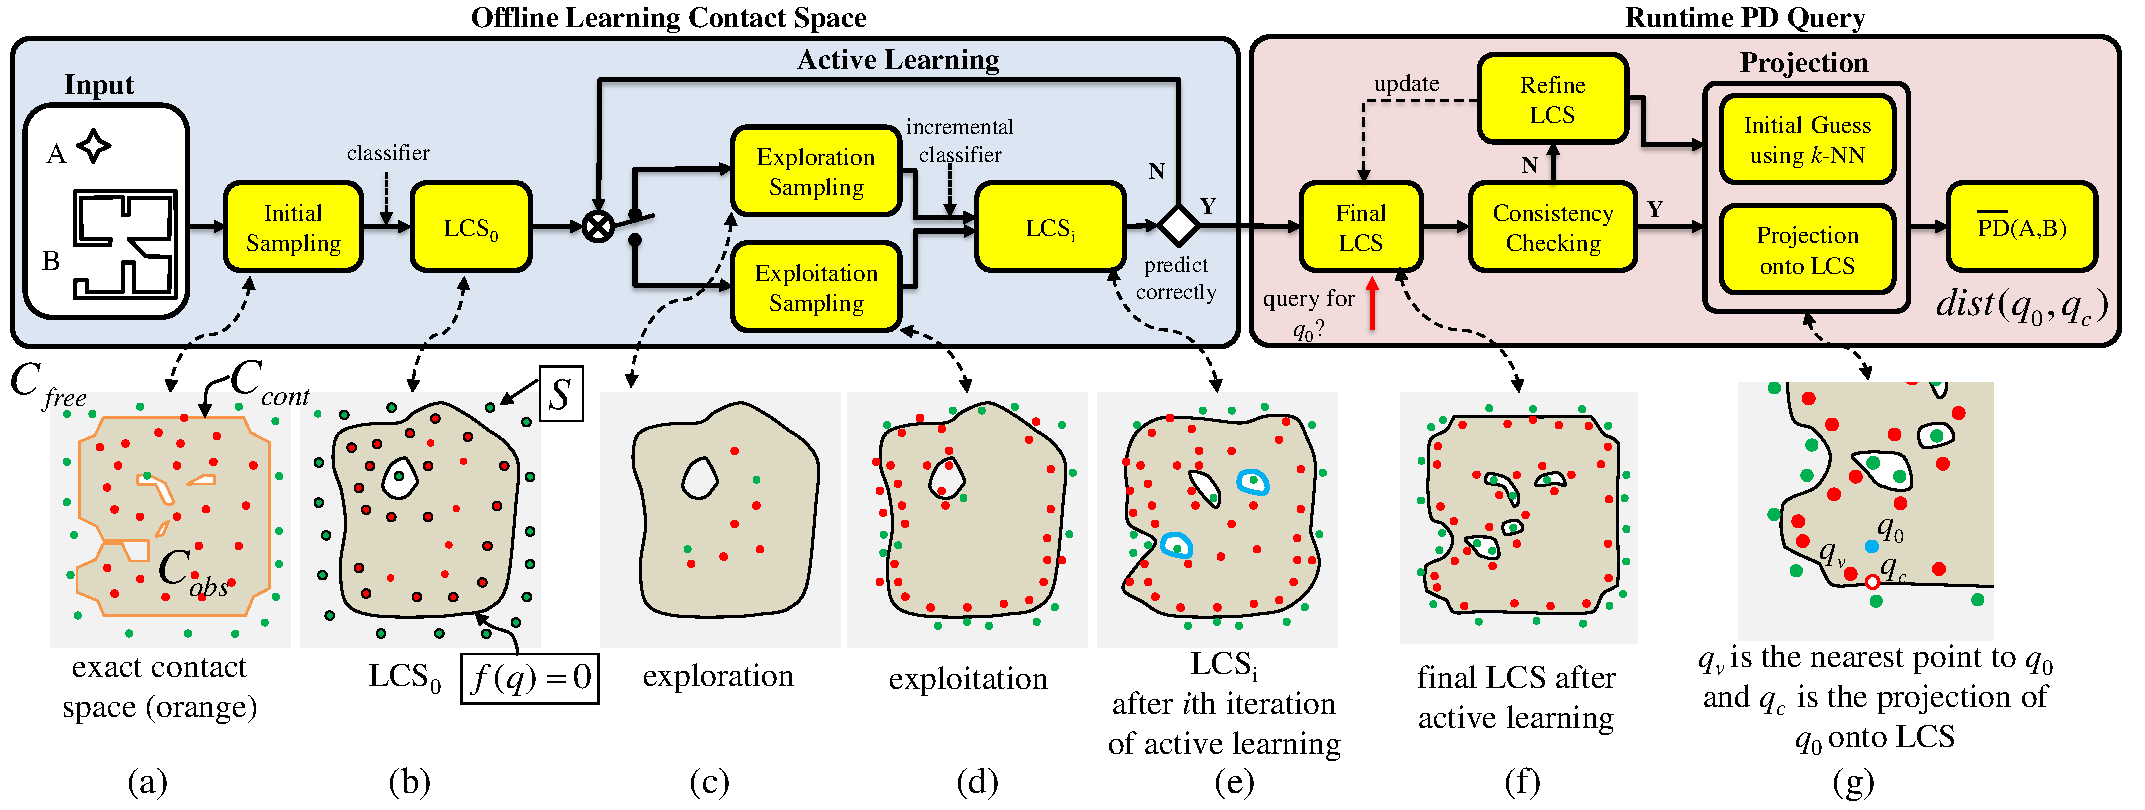
\includegraphics[width=\linewidth]{figs/2/pipeline.pdf}
  \caption[Offline computation pipeline for $\Ccont$ approximation and the runtime algorithm to compute the PD for a given query configuration]{This figure shows the offline computation pipeline for $\Ccont$ approximation and the runtime algorithm to compute the PD for a given query configuration. The different approximations of $\LCS$ are shown below the corresponding stages. We use green points to indicate collision-free configuration samples and red points to indicate in-collision samples.}
  \label{fig:2:pipeline}
\end{figure}

\section{Contact Space Construction via Machine Learning}
\label{sec:2:learning}
We now present our algorithm for the offline learning of the contact space and the computation of $\LCS$. Different stages of this algorithm
are shown in Figure~\ref{fig:2:pipeline}.

\subsection{Initial Sampling}
\label{sec:2:offline:uniform}

We perform uniform sampling in $\Cspace$ to obtain a set of configuration points. Rather than sampling the entire $\Cspace$,
we generate samples in a subspace that contains $\Ccont$. Given two objects $A$ and $B$, the contact space $\Ccont$ is contained in the in-collision space of their bounding volumes $BV(A)$ and $BV(B)$. We choose to use
axis-aligned bounding boxes (AABB) as the underlying BVs for $\PDt$
computation, due to their translational invariance in $\Rsqr$
and $\Rcubic$. Similarly, we use spheres as the underlying BVs for $\PDg$
computation due to their translational and rotational invariance in
$\SEsqr$ and $\SEcubic$.

The uniform sampling in the in-collision space of $BV(A)$ and $BV(B)$ can be implemented as follows. 
For $\PDt$ computation, the in-collision space of $BV(A)$ and $BV(B)$ is a box region, since it is the Minkowski sum of two axis-aligned bounding boxes. Samples uniformly distributed within this box region are guaranteed to cover the entire $\Ccont$.

For $\PDg$ computation, suppose that the given two bounding spheres are $(\mathbf c_A, r_A)$ and
$(\mathbf c_B, r_B)$, where $\mathbf c$ denotes a sphere center and $r$ denotes a sphere radius. We generate configuration samples for which these two bounding spheres are in collision. These samples correspond to all $(\mathbf R, \mathbf T)$ satisfying $\|\mathbf R \mathbf c_B + \mathbf T - \mathbf c_A\|_2 \leq r_A + r_B$, where $\mathbf R$ and $\mathbf T$ are the rotational and translational components of a configuration $\mathbf q$. We first generate one sample for the rotational component $\mathbf R$. For 2D rotation, we simply perform the uniform sampling within $[0, 2\pi]$; for 3D rotation, we use the method presented in~\cite{Shoemake:1992:URR} to sample $\SOcubic$ uniformly. After a random $\mathbf R$ is computed, the translational component $\mathbf T$ is uniformly distributed within a sphere $\|\mathbf T - (\mathbf c_A - \mathbf R \mathbf c_B)\| \leq r_A + r_B$; the uniform sampling within a sphere can be implemented using the well-known inverse-transform method. By repeating the above process many times, we can generate a sequence of $(\mathbf R, \mathbf T)$ uniformly distributed within the contact space of $A$ and $B$'s bounding spheres.

\subsection{Compute $\LCSa$} \label{sec:2:offline:model}
Given a set of $k$ samples from
$\Cobs(BV(A),BV(B))$, we perform exact collision queries between $A$ and $B$ to
check whether these samples are within in-collision space or not. Note that performing Boolean or discrete collision queries between complex models is a much easier problem compared to PD computation, as shown in Section~\ref{sec:2:analysis:timespacecomplexity}.
Our goal is to learn an approximate representation $\LCSa$ from these
configurations. In particular, $\LCSa$ corresponds to a decision function
$f(\q)=0$ that is fully determined by a set of configurations $\SV$
in $\Cspace$. We refer to $f(\q)$ as the \emph{classifier} and use it to
predict whether a given configuration $\q$ is collision-free
($f(\q)<0$) or in-collision ($f(\q)>0$). $\SV$ corresponds to the \emph{support vectors}, which are a
small subset of configuration samples used in learning.
Intuitively, $\SV$ are the samples that are closest to $\Ccont$.

Other options exist for computing the approximate contact space.
One alternative is to use surface fitting techniques to approximate the contact space by an implicit function, but this becomes more challenging for high-dimensional configuration spaces (e.g., 6-DOF $\Cspace$). Another possibility is to use regression-based learning techniques to approximate the contact space. However, such techniques typically require an improved or continuous approximation of PD values at these samples, which is much harder to compute compared to discrete collision queries.

\subsubsection{Nonlinear Classifier based on SVM}
\label{sec:2:offline:svm}
We use the SVM classifier~\cite{Vapnik:1995:NSL} to learn $\LCSa$ from
the initial sampling of $k$ configurations.
A SVM generates a decision function that is a smooth nonlinear surface. We use the
hard-margin SVM, as the underlying samples can
always be separated into collision-free and in-collision spaces. Intuitively, a SVM 
uses a function to map the given samples $\{\mathbf q_i\}$ from the \emph{input space} into a higher (possibly infinite) dimensional \emph{feature space}.
A SVM computes a linear
separating hyperplane characterized by parameters $\mathbf w$ and $b$. The hyperplane's maximal margin
is in the higher dimensional feature space. The hyperplane corresponds to a nonlinear separating surface in the input space. The $\mathbf w$ is the normal vector to the hyperplane, and the
parameter $b$ determines the offset of the hyperplane from the
origin along the normal vector. In the feature space, the distance between a hyperplane and the closest sample point is
called the `margin', and the optimal separating hyperplane should maximize this distance.
The maximal margin can be achieved by solving the following
optimization problem:
\begin{align}
\label{eq:2:svm1}
& \underset{\mathbf w, b}{\text{min}} & & \frac{1}{2}\|\mathbf w\|^2 & &  \\
& \text{subject to} & & c_i (\mathbf w \cdot \phi(\mathbf q_i) + b)
\geq 1, & & 1 \leq i \leq k. \notag
\end{align}
where $c_i \in \{-1,+1\}$ is the collision state of each sample ${\mathbf q_i}$.

Let $K(\mathbf q_i, \mathbf q_j) = \phi(\mathbf q_i)^T
\phi(\mathbf q_j)$ represent the kernel function (i.e., a function
used to calculate inner products in the feature space). The distance
between two points $\phi(\mathbf q_i)$ and $\phi(\mathbf q_j)$ in
the feature space can be computed as:
\begin{flalign}
\label{eq:2:svmdist}
&\|\phi(\mathbf q_i)-\phi(\mathbf q_j)\| \nonumber\\
&= \sqrt{K(\mathbf q_i, \mathbf q_i) + K(\mathbf q_j, \mathbf q_j)
- 2 K(\mathbf q_i, \mathbf q_j)}.
\end{flalign}
In our algorithm, we use the radial basis function (RBF) as the kernel:
$K(\mathbf q_i, \mathbf q_j) = \exp(-\gamma \|\mathbf q_i - \mathbf
q_j\|^2)$, where $\gamma$ is a positive parameter. In practice, we use $\gamma = 20$. We use the RBF kernel because it maintains the distance ranking
in both the input space and the feature space due to the fact that $\|\phi(\mathbf q_i) - \phi(\mathbf q_j)\|_2^2 = 2 - 2 \cdot \exp(-\gamma \|\mathbf q_i - \mathbf q_j\|_2^2)$.

The solution of Equation~\ref{eq:2:svm1} is a nonlinear surface in the
input space (and a hyperplane in the feature space) that separates
collision-free and in-collision configurations. This solution can be
formulated as:
\begin{align}
\label{eq:2:svmf} f(\mathbf q) = \mathbf w^* \cdot \phi(\mathbf q) +
b^* = \sum_{i=1}^k \alpha_i c_i K(\mathbf q_i, \mathbf q) + b^*,
\end{align}
where $\mathbf w^*$ and $b^*$ are the solutions of
Equation~\ref{eq:2:svm1} and $\alpha_i \geq 0$. 
The vectors $\mathbf q_i$ corresponding to the non-zero $\alpha_i$ are called
the \emph{support vectors}, which we denote as $\SV$. Intuitively, the support vectors
are those samples closest to the separating hyperplane
$f(\mathbf q) = 0$, as shown by the larger red and green points in
Figures~\ref{fig:2:pipeline}(b) and ~\ref{fig:2:pipeline}(g).
Thus, $\LCSa$ consists of an implicit function
$f_{\LCSa}(\q) = f(\q)$ and a set of samples
$S_{\LCSa}=S$ (i.e., the support vectors), which
are used to approximate the exact contact space.


\subsection{Refine $\LCSa$ using Active Learning}
\label{sec:2:offline:activelearning}
We refine $\LCSa$ using active learning. The
goal is to actively select new samples so that a better
approximate contact space representation, $\LCSb$, can be obtained by incorporating
these samples into $\LCSa$. We use a
combination of exploration and exploitation~\cite{Huang:2010:ALQ}.
The idea is to determine whether to explore
or to exploit by flipping a biased coin with a certain probability for landing on heads
(initially $0.5$). If the result is a head, we apply exploration;
if it is a tail, we apply exploitation. The probability of landing on heads is adjusted
according to the fraction of exploration samples' collision
states that are correctly predicted by the current $\LCSi$. The new
samples are used to update $\LCSa$ and generate a new approximation
$\LCSb$ (or refine from $\LCSi$ to $\LCSiplus$). We repeat the active
learning step until all the new samples can either be correctly
predicted by the current $\LCSi$, or the final result (represented
as $\LCS$) has sufficient accuracy to approximate $\Ccont$. Later in Section~\ref{sec:2:analysis}, we show that active learning results in improved convergence compared to uniform or random sampling schemes.


\subsubsection{Exploration}
$\LCSa$ may miss some holes or components corresponding to collision-free regions, if no initial samples were generated inside those regions. As a result, there may be some portions that $\LCSa$ may incorrectly classify, as shown in Figure~\ref{fig:2:pipeline}(c). In this case,
exploration refers to generating samples far away from prior
samples in order to explore the regions not well-sampled by the
current $\LCSi$. In our algorithm, we use random sampling to
explore these new regions (Figure~\ref{fig:2:pipeline}(c)). As
shown in Figure~\ref{fig:2:pipeline}(e), two new collision-free
regions (marked as blue curves) are found using exploration. After
each exploration sampling step, we compute the fraction of the new
samples that are not correctly predicted by $\LCSi$ to determine whether the exploration improves $\LCSiplus$.
If this cutoff fraction is large (e.g., $0.3$), then we increase the probability for exploration; otherwise we
decrease it.


\subsubsection{Exploitation}
Exploitation refers to generating samples near the decision
function of a given approximation $\LCSi$.

For exploitation, we use a simple method based on the \emph{maximal margin} property
of SVMs. The maximal margin
property~\cite{Vapnik:1995:NSL} states that in the feature space, the decision function
will have the same distance to support vectors with different
labels (i.e., collision-free or in-collision). In order to obtain a sample near the
decision function $f_{\LCSa} = 0$, we first choose a pair of support
vectors that are close to each other, but have opposite labels.
Based on the maximal margin property, the midpoint of the two
supporting vectors lies on or near the decision function.
\begin{figure}[!htb]
  \centering
  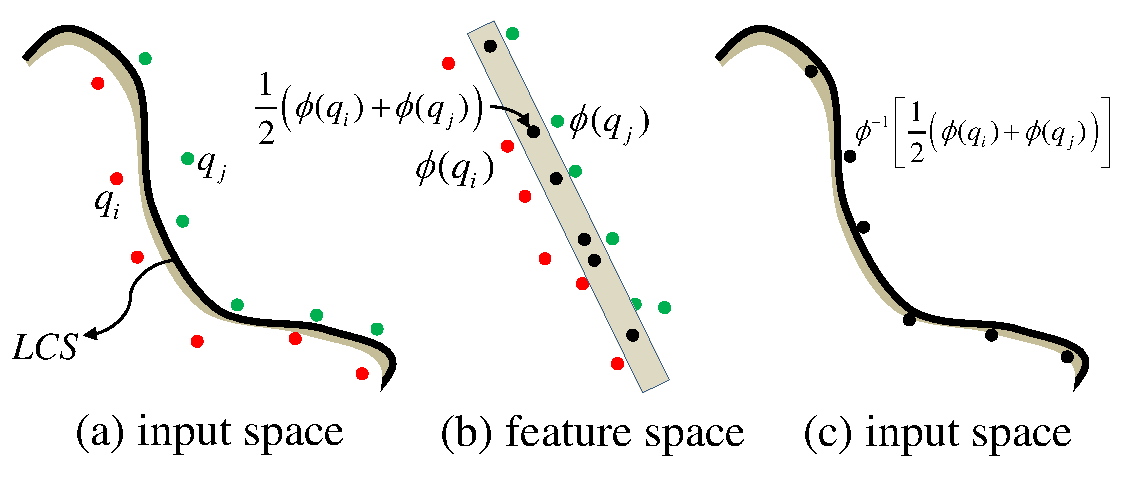
\includegraphics[width=0.6\linewidth]{figs/2/interpolation.pdf}
  \caption[Exploitation in SVMs]{Exploitation in SVMs:
  (a) support vectors are on different sides of the decision function ($\mathbf q_i$ and $\mathbf q_j$) in the input space;
  (b) their midpoints (black points) are computed in the feature space;
  (c) the pre-images of the midpoints lie near the decision function and can be used for exploitation.}
  \label{fig:2:interpolation}
\end{figure}
For nonlinear SVMs, the closest point and interpolation computations are
performed in the feature space. As shown in
Figure~\ref{fig:2:interpolation}, we first use the distance metric
mentioned in Equation~\ref{eq:2:svmdist} to find a pair of
supporting vectors $\mathbf q_i$ and $\mathbf q_j$. Next, we
compute their midpoint $\frac{1}{2}(\phi(\mathbf q_i) +
\phi(\mathbf q_j))$ (shown as black points in Figure~\ref{fig:2:interpolation}(b)). However, since the resulting midpoint may not have a pre-image in the input space, we search the input
space for a point $\q$ whose image $\phi(\q)$ in
feature space is closest to $\frac{1}{2}(\phi(\mathbf q_i) +
\phi(\mathbf q_j))$:
\begin{equation}
\begin{aligned}
\label{eq:2:preimage}
& \ \underset{\mathbf q}{\text{min}} & & \|\frac{1}{2}(\phi(\mathbf q_i) + \phi(\mathbf q_j)) - \phi(\mathbf q)\|_2 & \\
\Leftrightarrow & \ \underset{\mathbf q}{\text{max}} & & K(\mathbf q, \mathbf q_i) + K(\mathbf q, \mathbf q_j). &
\end{aligned}
\end{equation}
The solution is found using an optimization solver, in which the midpoint $\frac{\mathbf q_i +
\mathbf q_j}{2}$ in the input space is used as the initial guess. In our
benchmarks, this optimization solver tends to converge quickly
(in less than $10$ iterations).


\subsection{Incremental Learning}
\label{sec:2:incremental_learning}
Instead of computing a new decision function
from scratch using all the previous samples, we apply incremental
learning techniques to efficiently compute $\LCSiplus$ from
$\LCSi$. Incremental learning utilizes a small set
of new samples to update $\LCSi$. The decision function of $\LCSi$
serves as the initial guess for generating $\LCSiplus$. The incremental SVM~\cite{Karasuyama:2009:MID} can update
the current result generated using SVMs; the key is to retain the optimality condition of Equation~\ref{eq:2:svm1} (i.e., the Kuhn-Tucker condition) on all prior samples while adding new samples. This is achieved by adjusting the coefficients $\alpha_i$ and $b$ in Equation~\ref{eq:2:svmf} and by adjusting support vector set $\SV$. The coefficient adjustment and the support vector changes are guided by the gradient of the objective function in Equation~\ref{eq:2:svmf}.

\subsection{Terminating Active Learning}
Active learning terminates when either of these conditions has been satisfied:
\begin{enumerate}
    \item The collision states of all the new samples generated during
exploration and exploitation can be correctly predicted by the
current approximation $\LCSi$.
    \item The total number of samples used in active learning iterations is more than a user-specified threshold.
   \end{enumerate}
The first condition guarantees that all the configurations used for learning $\LCS$ are consistent (i.e., they can be correctly predicted by $\LCS$). This implies that the current $\LCS$ is a close approximation of the underlying contact space.
The second condition controls the error in PD computation. As more samples are used, we get a better approximation to $\Ccont$, and thereby a lower PD error.


\section{Approximate PD Computation}
\label{sec:2:approxPD}

We use the learned approximate contact space $\LCS$ to perform PD queries at
runtime. This section describes details on the runtime
algorithm. It consists of two parts: local $\LCS$ refinement based on consistency checks, and
computing the nearest configuration on $\LCS$.


\subsection{Local $\LCS$ Refinement}
Let $\qa$ be a configuration that corresponds to overlapping rigid objects $A$
and $B$. The exact collision check between these objects is performed using
bounding volume hierarchies. We also compute the approximate collision state corresponding to $\qa$ using $\LCS$: i.e., we
check whether ($f(\qa)>0$) as that corresponds to an in-collision configuration.
It is possible that the collision state predicted
using $\LCS$ may be different from that computed by the exact
algorithm, which implies that $\LCS$ is not sufficiently
accurate at approximating the contact space in the neighborhood of $\qa$.
In this case, we refer to $\qa$ as an \emph{inconsistent} configuration;
otherwise, it is consistent.
Generally, an inconsistent configuration occurs when the query is located in
a $\Cspace$ region that is not well sampled during the learning phase.

Our runtime algorithm first checks
whether a given query $\qa$ is consistent. If $\qa$ is inconsistent, $\qa$ corresponds to a collision-free configuration
predicted by $\LCS$ ($f(\qa)<0$) and its distance to $\LCS$ is
more than a user-specified error threshold. In this case, we locally refine
$\LCS$ by incorporating $\qa$ into $\LCS$ using incremental learning (Section~\ref{sec:2:incremental_learning}).
This local refinement of $\LCS$ improves the query efficiency and the accuracy of PD computation (Equation~\ref{eq:2:Errdef}).

During each runtime query, we perform an incremental learning step for an inconsistent
single configuration. This incremental learning has an runtime overhead of $\mathcal O(1)$.
Moreover, this local refinement step improves the accuracy of $\LCS$ in local
regions where more PD queries are potentially performed by an application during runtime. 
As a result, this step results in more accurate answers for those nearby queries by exploiting the spatial coherence in the configuration space.

\subsection{$\LCS$ Projection}
\label{sec:2:approxPD:projection}
Given a consistent configuration $\qa$, we search for the closest configuration
on $\LCS$ to compute the PD. In particular,
we \emph{project} $\qa$ onto the decision boundary $f_{LCS} = 0$ to obtain $\qc$, the nearest configuration on $\LCS$. In this case, the approximate
PD is computed using $\dist(\qa, \qc)$ function.
For SVM classifiers, the projection computation can be reduced to a constrained
optimization problem:
\begin{equation}
\begin{aligned}
\label{eq:projection}
 & \underset{\mathbf q}{\text{min}} & \dist(\mathbf \qa, \mathbf q), & & \text{subject to} & & f_{LCS}(\mathbf q) = 0.
\end{aligned}
\end{equation}
A key challenge is to perform this projection efficiently and ensure that the optimization algorithm is not
trapped in a local minima, as the shape of the decision function can be complicated.
In order to deal with these issues, we perform the computation in two phases:
first, we perform a $k$-nearest-neighbor search in $\Cspace$ to compute the configuration
$\qv \in S_{LCS}$ (i.e., the configuration among the support vectors) that is closest to $\qa$ based on our $\dist(\cdot, \cdot)$ metric. Next, we
use $\qv$ as an initial guess to the constrained optimization problem and compute the closest configuration on the $\LCS$.
Since $\qv$ is a configuration very close to the decision boundary, it serves as a good initial guess.

We use different nearest-neighbor (NN)  search algorithms to compute $\qv$, depending on whether we are
performing this search in 3-DOF $\Cspace$ or 6-DOF $\Cspace$. For 3-DOF $\Cspace$, $\dist(\cdot, \cdot)$ corresponds to the Euclidean distance metric, and we use a kd-tree to accelerate NN computation. For 6-DOF $\Cspace$, we use a hierarchical clustering algorithm for efficient NN search~\cite{Muja:2009:FAN}.

\section{Analysis}\label{sec:2:analysis}
In this section, we analyze various characteristics of our algorithm, including errors in PD computation, benefits of active learning, and time and space complexity.

\subsection{Error in $\LCS$ and in PD Computation}
\label{sec:errordefine}
Since our approach is probabilistic, we compute a bound on PD approximation based on \emph{expected
error}~\cite{Vapnik:1995:NSL}, which corresponds to the average error
when $\LCS$ is applied to predict the
collision state or PD value for a new configuration in the $\Cspace$.
This error can be expressed as:
\begin{equation}
\label{eq:2:Errdef0} e_{\text{col}} = \mathbb E
\left|e_\text{cs}(\mathbf q) \right|,
\end{equation}
where $e_{\text{cs}}(\q)=0$ if $\q$ is a consistent configuration, and $e_{\text{cs}}(\q)=1$ if $\q$ is inconsistent.
Expectation $\mathbb E$ is calculated from a series of
random configurations or queries. Typically, these queries arise from an application (e.g., dynamic simulation), and
we assume that they follow a uniform distribution in $\Cspace$.

The accuracy of approximate global PD computation is measured by the expected error that arises
when using $\LCS$ to compute the PD for a random configuration in $\Cspace$:
\begin{equation}
\label{eq:2:Errdef} e_{\text{PD}} = \mathbb E
\left|\overline{\text{PD}}(A(\q), B) - \text{PD}(A(\q), B)\right|.
\end{equation}
Note that we scale the objects such that the maximum dimension of the subspace $\Cobs (BV(A),BV(B))$ is equal to 1.
The accuracies of approximate global PD and approximate contact space are closely related: a small value of $e_{\text{col}}$ implies a small value of $e_{\text{PD}}$ and vice versa.

\begin{figure}[!h]
\begin{center}
\subfloat[$e_{\text{col}}$ for 2D spiders]{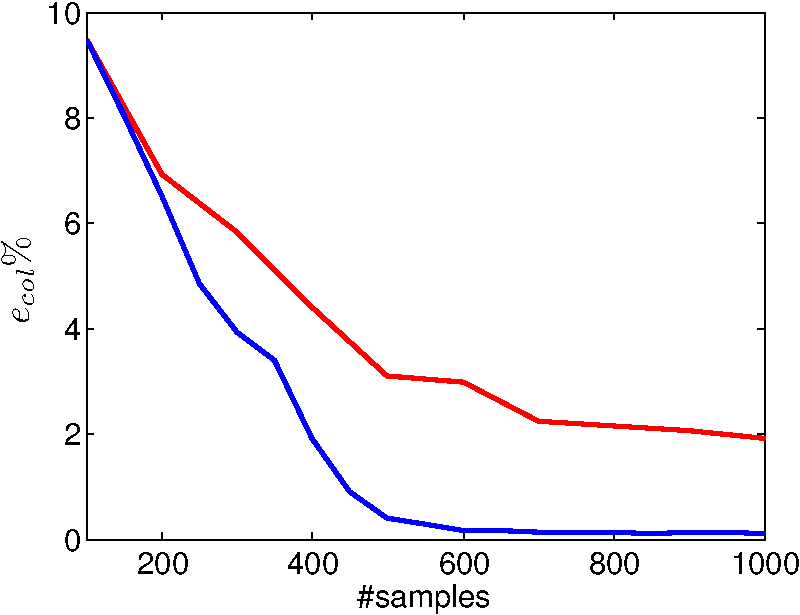
\includegraphics[clip=true, width=0.43\textwidth]{figs/2/active/spider_activelearning-crop.pdf}}
\subfloat[$e_{\text{col}}$ for 3D cup-spoon]{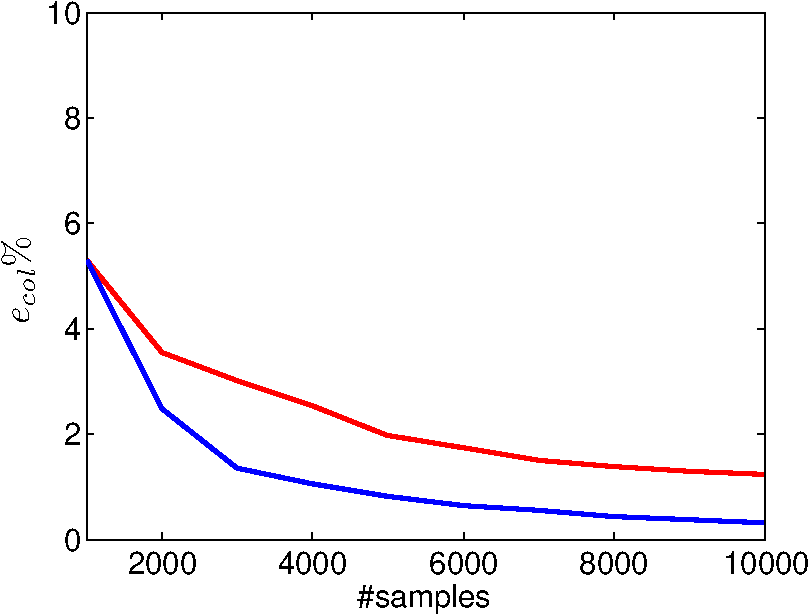
\includegraphics[clip=true, width=0.43\textwidth]{figs/2/active/cupspoon_activelearning-crop.pdf}}
\end{center}
\caption[Relative error convergence of active learning vs. uniform sampling for 2D and 3D object pairs]{Relative error convergence of active learning (blue) vs. uniform sampling (red) for 2D and 3D object pairs. These results demonstrate the benefits of active learning in terms of requiring fewer samples and improved accuracy.}
\label{fig:2:activelearningtime}
\end{figure}

\subsection{Benefits of Active Learning}
A key component of our algorithm is the computation of $\LCS$ by generating appropriate samples in the configuration space. The simplest choice is to perform uniform sampling in $\Cobs (BV(A),BV(B))$ or to use some other random sampling scheme. Instead, we use a combination of active and incremental learning techniques to refine $\LCSi$ and improve its accuracy.


The time and space complexity of the $\LCS$ precomputation phase is a function of
the number of samples used for active learning iterations. The number of samples required to achieve a given error bound $e_{\text{col}}$ depends on both the active learning technique and the underlying classification method used within active learning iterations. It is non-trivial to derive a tight bound on the number of samples required for a specific combination of active learning and classification algorithms. However, we use general results on the sample complexity of active learning~\cite{Hanneke:2013} to show the benefits of our approach.
\begin{theorem}
\label{thm:2:activelearning}
If the number of samples used in active learning iterations of $\LCS$ computation is more than $N$,
where $N=\mathcal O(\log(1/(\epsilon \delta))$, then there exists one active learning technique which can guarantee that with probability at least $1-\delta$, the expected error of the $\LCS$ result will satisfy the bound $e_{\text{col}}\leq\epsilon$.
\end{theorem}

Intuitively, this theorem states there exists a particular active learning technique that will achieve a given bound on $\LCS$ approximation error with high probability.
A proof of this theorem can be obtained based on the CAL (Cohn-Atlas-Ladner) algorithm~\cite{Cohn:ML:1994}. Our $\LCS$ computation is guaranteed to satisfy a bounded error with high probability, if more than $N=\mathcal O(\log(1/(\epsilon \delta))$ samples are used. However, the CAL active learning algorithm is not practical~\cite{Hanneke:2013} and rather we use a combination of exploration and exploitation for active learning (Section~\ref{sec:2:offline:activelearning}) in our $\LCS$ computation algorithm.

Many applications use exploration and exploitation for active learning algorithms. We expect that the use of exploration and exploitation likely also results in a bound similar to Theorem~\ref{thm:2:activelearning}, although the exact derivation of such a bound is a good topic for future research.

Since $e_{\text{col}}$ and $e_{\text{PD}}$ are closely related to each other, Theorem~\ref{thm:2:activelearning} also implies that
$e_{\text{PD}}$ decreases exponentially with the number of samples.
In contrast, when using a uniform sampling strategy to learn the contact space, 
$\LCS$ converges to the
exact contact space
at a polynomial rate as the number of samples
increases~\cite{Mohri:2012:FML}:
\begin{theorem}
\label{thm:2:uniform}
When using uniform sampling, if the number of samples is more than $N$, where $N = \mathcal O(
\frac{1}{2\epsilon^2} \log(2/\delta))$, then
with probability $\geq 1- \delta$, we have the error bound $e_{\text{col}} \leq
\epsilon$.
\end{theorem}

We also measured the expected errors, $e_{\text{col}}$ and $e_{\text{PD}}$, in
complex 2D and 3D benchmarks, as shown in Figure~\ref{fig:2:activelearningtime}.
This demonstrates the high convergence rate and lower error in $\LCS$ computation and PD computation using active learning given the same number
of samples.

\subsection{Benefits of Local Refinement}
Our contact space and PD computation approaches are probabilistic algorithms. Their accuracy is determined by
the samples chosen during the learning phase, including the initial samples and active learning as well as
the runtime queries. As more PD queries are performed within a subspace or a specific region of $\Cspace$,
the accuracy of $\LCS$ in that subspace or region tends to become higher.
This is due to the local refinement step that is performed during runtime whenever we encounter an
inconsistent query configuration.
The incremental learning algorithm updates $\LCS$ around the query configuration by taking into account
local information in $\Cspace$.
In many applications, including dynamic simulation, haptics, or motion planning, a high proportion of
sample queries correspond to positions near the two objects $A$ and $B$. As a result, the runtime
query configurations are relatively close to each other in $\Cspace$ and the local refinement
step improves the accuracy of $\LCS$ in that region. This implies that as more queries are performed in
a localized region of $\Cspace$, the accuracy of $\LCS$ and PD queries improves.
Our algorithm does not make any assumptions about the application or the distribution of runtime query
configurations. We expect that the accuracy of local refinement will improve at the rate given by
uniform sampling (i.e., Theorem~\ref{thm:2:uniform}), rather than at the exponential rate of active learning.
In other words, after generating $N = \mathcal O(1/\epsilon^2)$ samples within a subspace at runtime,
the expected error locally around those samples should be less than $\epsilon$.


\subsection{Time and Space Complexity}
\label{sec:2:analysis:timespacecomplexity}
The precomputation or learning phase is performed for each object pair $(A, B)$
in the environment. The exact collision check is performed using precomputed bounding volume hierarchies.
Given two objects represented as meshes with $m$ and $n$ triangles, the expected cost of a single
exact collision query is $T_{col} = \mathcal O(\log m + \log n)$.

\begin{figure}[!htb]
\begin{center}
\subfloat[$\LCS_0, |S| = 88$]{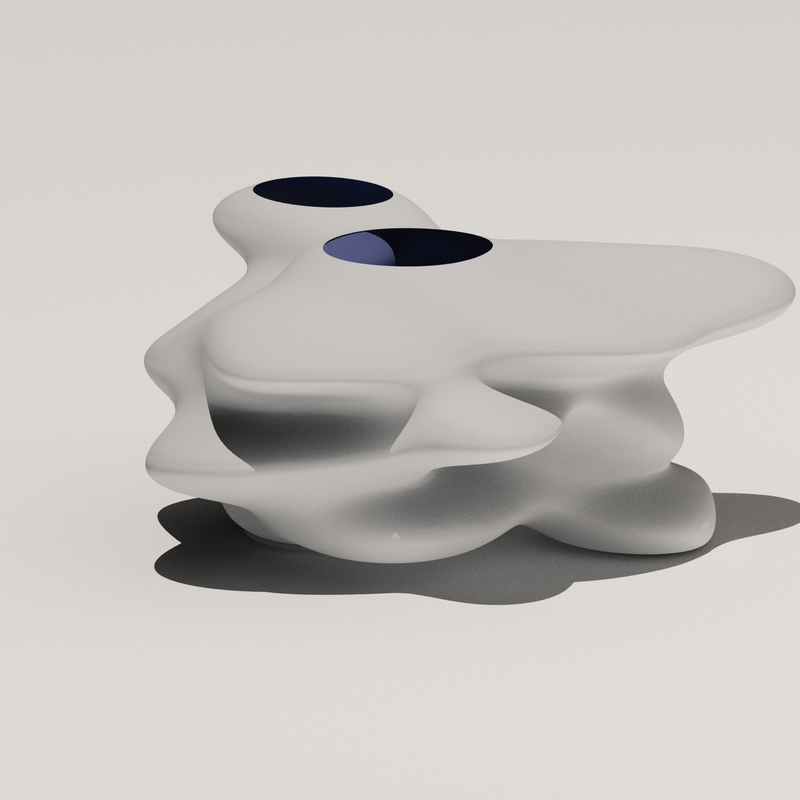
\includegraphics[width=0.24\linewidth]{./figs/2/LCSPDg2D_StarRoom/LCS0.png}}
\subfloat[$\LCS_5, |S| = 174$]{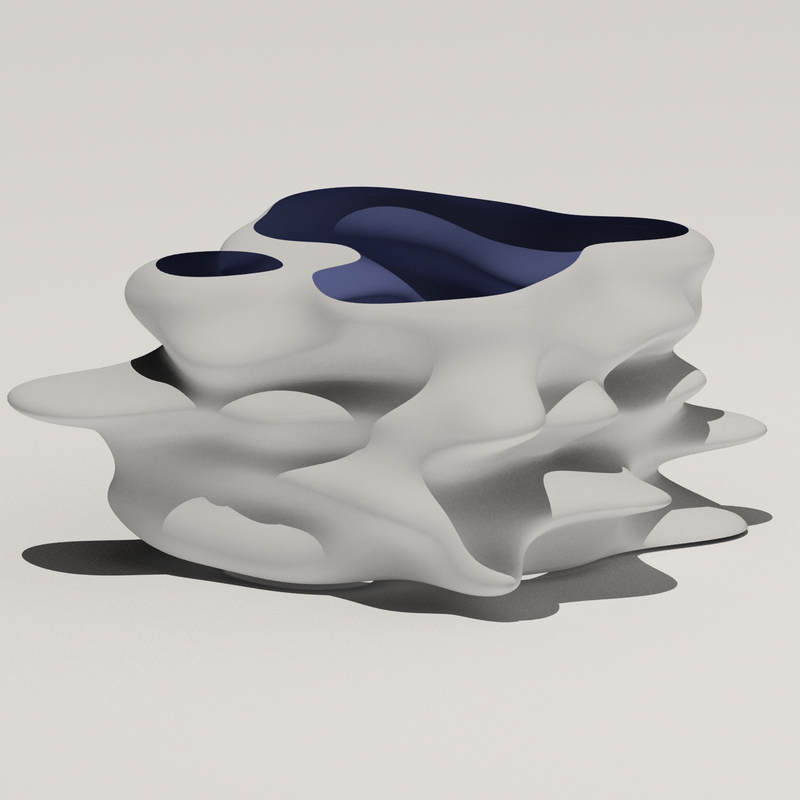
\includegraphics[width=0.24\linewidth]{./figs/2/LCSPDg2D_StarRoom/LCS5.png}}
\subfloat[$\LCS_9, |S| = 237$]{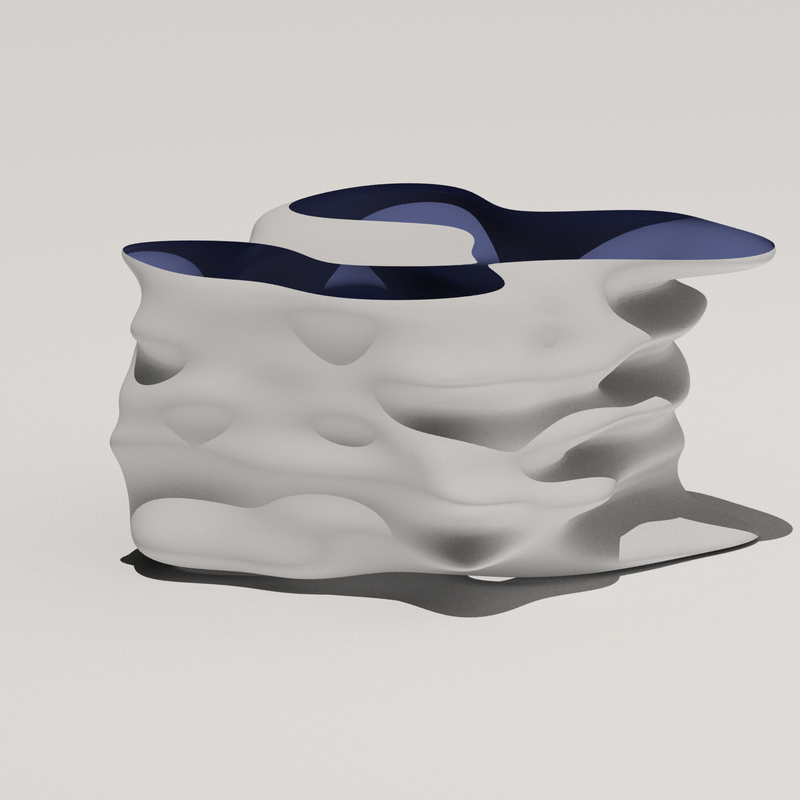
\includegraphics[width=0.24\linewidth]{./figs/2/LCSPDg2D_StarRoom/LCS9.png}}
\subfloat[$\LCS_{12}, |S| = 248$]{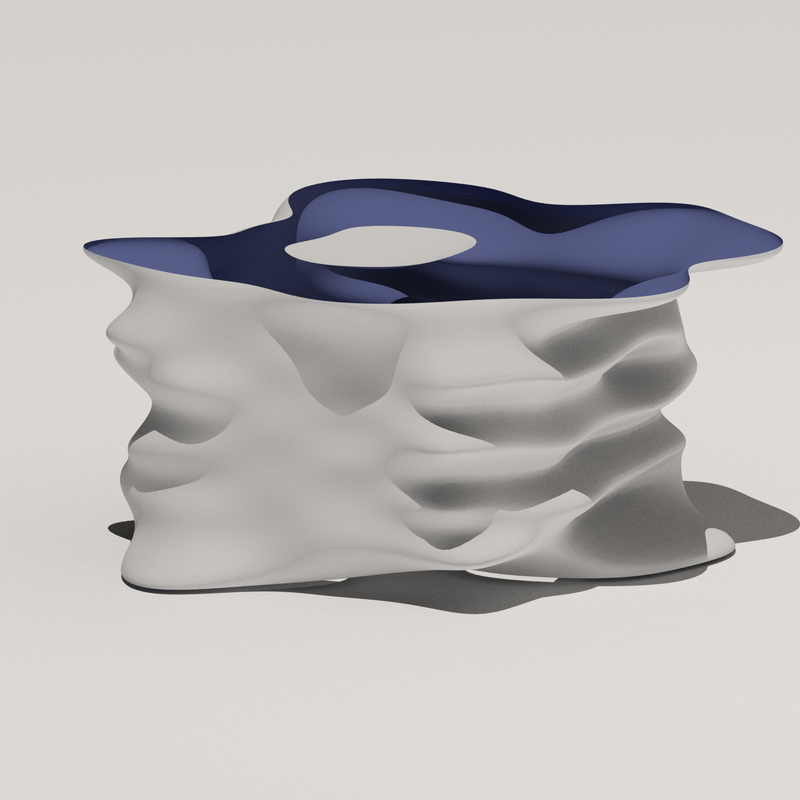
\includegraphics[width=0.24\linewidth]{./figs/2/LCSPDg2D_StarRoom/LCS18.png}}
\caption[$\LCS$ computation using active learning for $\PDg$ query between 2D non-convex shapes]{$\LCS$ computation using active learning for $\PDg$ query between 2D non-convex shapes given in Figure~\ref{fig:2:pipeline}. We show the approximation after $i$-th iteration and the number of support vectors. The vertical axis represents the rotational component of the $\Cspace$. }
\label{fig:2:LCSinActiveLearning2D2}
\end{center}
\end{figure}

\begin{figure}[!htb]
\begin{center}
\subfloat[$\LCS_0, |S|=231$]{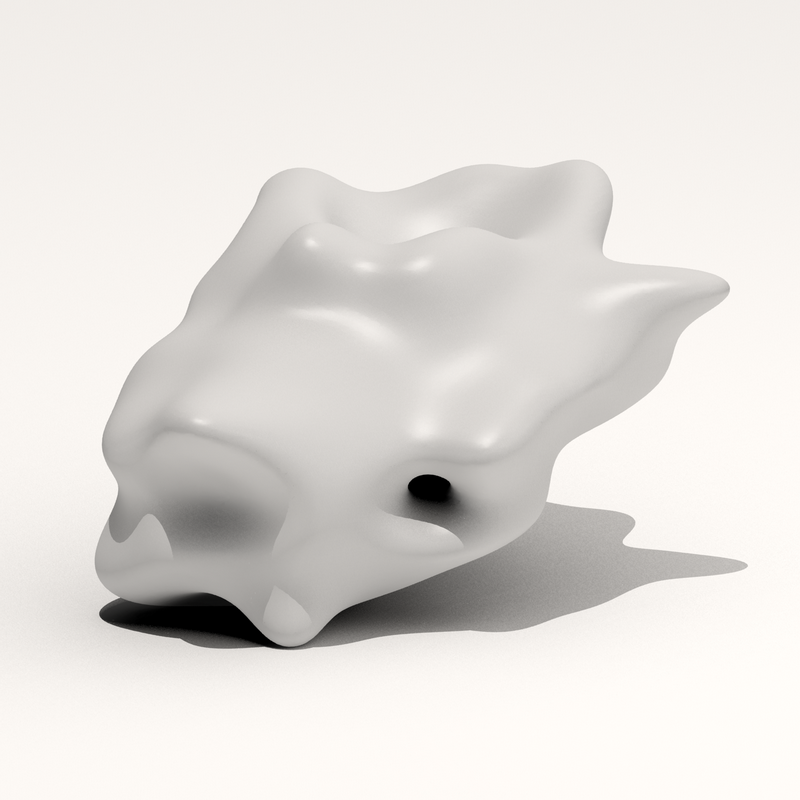
\includegraphics[width=0.24\linewidth]{./figs/2/LCSPDt3D_CupSpoon/LCS0.png}}
\subfloat[$\LCS_5, |S|=869$]{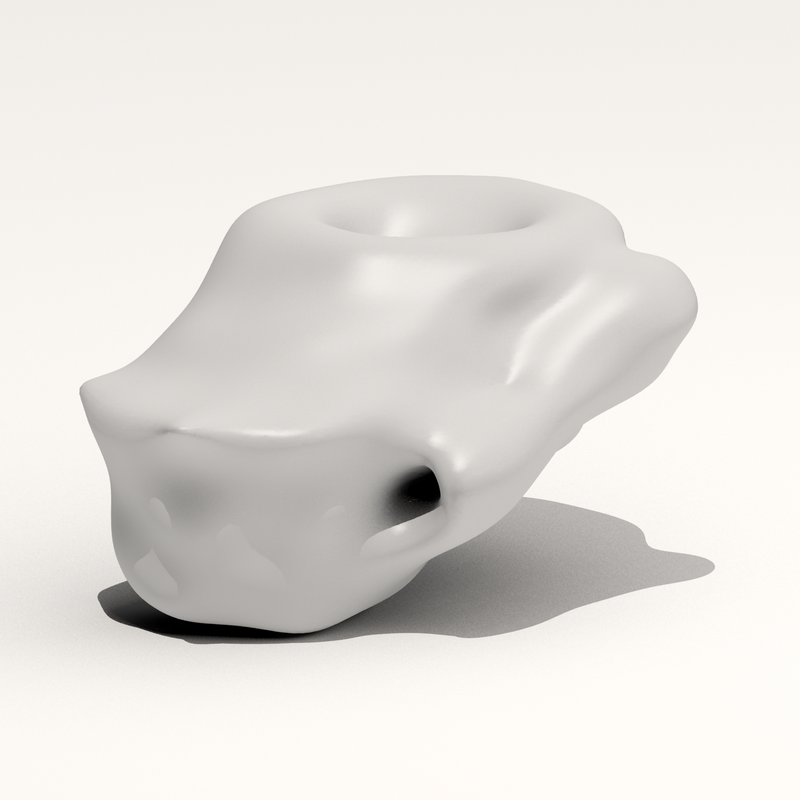
\includegraphics[width=0.24\linewidth]{./figs/2/LCSPDt3D_CupSpoon/LCS5.png}}
\subfloat[$\LCS_9, |S|=1350$]{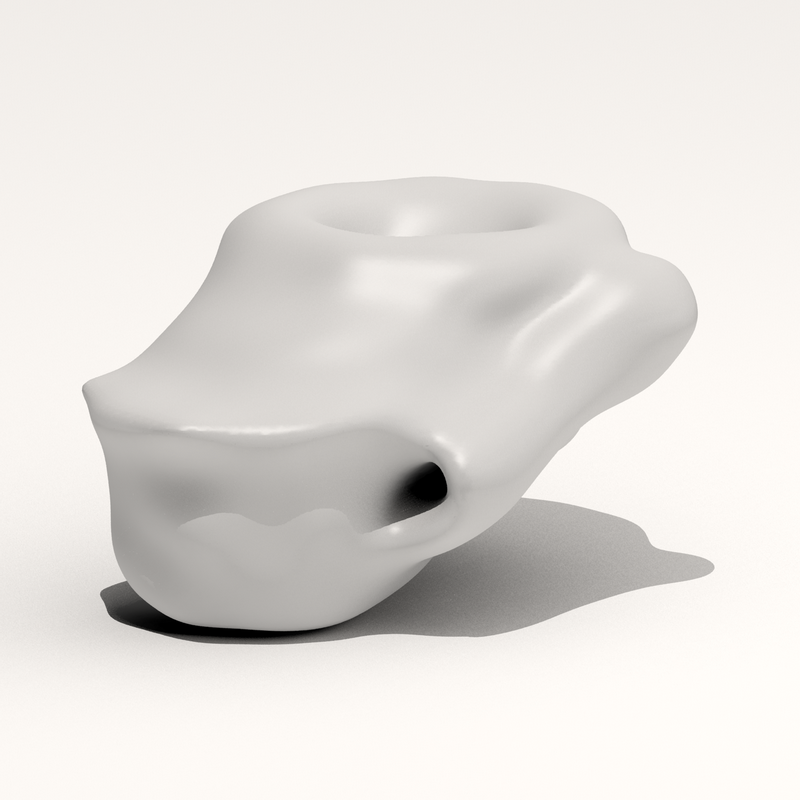
\includegraphics[width=0.24\linewidth]{./figs/2/LCSPDt3D_CupSpoon/LCS10.png}}
\subfloat[$\LCS_{12}, |S|=1572$]{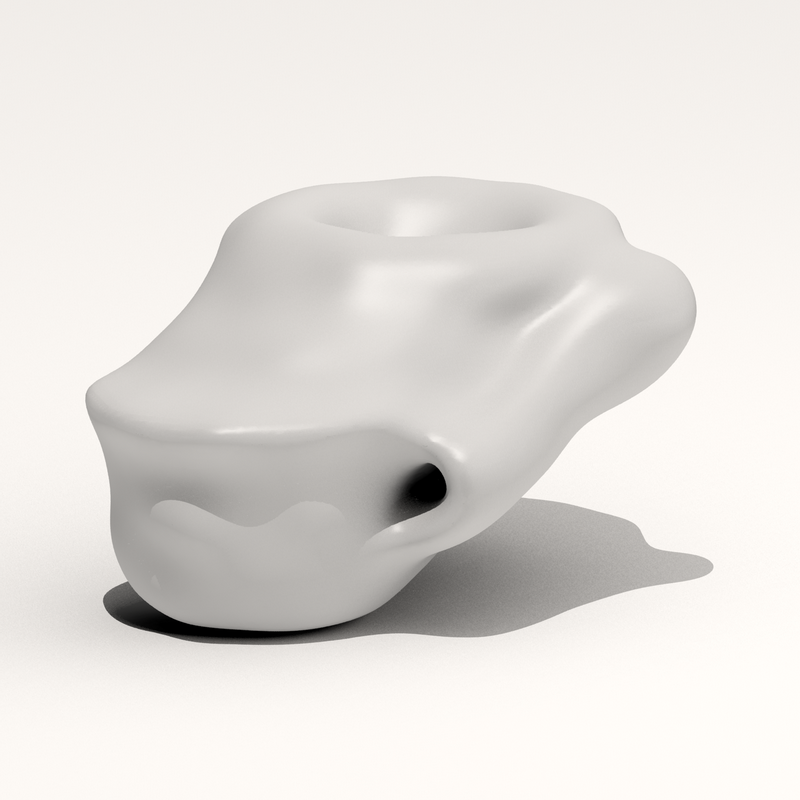
\includegraphics[width=0.24\linewidth]{./figs/2/LCSPDt3D_CupSpoon/LCS17.png}}
\caption[$\LCS$ computation using active learning for $\PDt$ query between 3D cup and spoon]{$\LCS$ computation using active learning for $\PDt$ query between 3D cup and spoon. We provide the number of support vectors corresponding to $\LCSi$. As shown, the algorithm can compute a good approximation in a few iterations.}
\label{fig:2:LCSinActiveLearning3D}
\end{center}
\end{figure}


\paragraph{Offline Learning:} The time complexity for the learning
phase can be estimated as
\begin{align} \label{eq:2:cost}
(T_{LCS_0} + \sum_{i=1}^{I_{AL}} (T_{ES_i} + T_{LCS_i})) + T_{col} \cdot \sum_{i=1}^{I_{AL}} N_{LCS_i},
\end{align}
where $T_{LCS_0}$ is the time complexity to learn the initial approximation;
$T_{ES_i}$ is the time cost to perform exploitation sampling or
exploration sampling in the $i$-th iteration of active learning;
$T_{LCS_i}$ is the time cost for the $i$-th step of incremental
learning, and $I_{AL}$ is the number of iterations performed during active
learning. We denote the number of new samples generated
during $LCS_i$ as $N_{LCS_i}$. We perform collision checking for each sample generated during the learning phase; hence the collision cost is
$T_{col} \cdot \sum_i N_{LCS_i}$.

$T_{LCS_0}$ complexity is governed by the SVM classifier. SVM computation boils down
to solving a constrained quadratic optimization problem using the interior
point or conjugate gradient method, and its worst-case complexity
is $\mathcal O(N_{LCS_0}^{2.3})$.

Incremental learning combines each new sample into $\LCS$ in
constant time, and hence we have $T_{LCS_i} = \mathcal
O(N_{LCS_i})$. $T_{ES_i}$ is the time cost for exploitation sampling
or exploration sampling. For exploration, $T_{ES_i} = \mathcal
O(N_{LCS_i})$. The time complexity for exploitation sampling is
$\mathcal O(|S_{LCS_i}|)$ as we perform interpolation between each
support vector of $\LCSi$ and its $k$-nearest neighbors, which can
be bounded from above as $\mathcal O(\sum_i N_{LCS_i})$.

Overall, the time complexity for the learning phase is
$\mathcal O(\log(\frac{1}{\epsilon}) \sum_i{N_{LCS_i}} +
N_{LCS_0}^{2.3}) + T_{col} \cdot \sum_i N_{LCS_i}$.
The space complexity of our algorithm is linear in the
number of samples used during the learning and runtime phases, and is linear in the number of support vectors in the final $\LCS$ representation.

\paragraph{Runtime Query:} The time complexity in the runtime query
phase depends on $\left| S_{LCS} \right|$, i.e., the number of
support vectors in $\LCS$. $\left| S_{LCS} \right|$ depends on
the smoothness of the exact $\Ccont$, and not as much on the geometric complexity of $A$ and $B$ (see Figures~\ref{fig:2:LCSinActiveLearning2D2} and~\ref{fig:2:LCSinActiveLearning3D}).
For example, the $\Ccont$ of a sphere and another object (i.e., the offset surface) is always smooth, and
therefore a small $\SVLCS$ is sufficient to generate a good approximation of $\Ccont$.
We also notice this in our benchmarks, where $|S|$ for the teeth model (40K triangles) is comparable or higher than that for the bunny (70K triangles), dragon (230K triangles), and Buddha (1M triangles) models. Furthermore, we generated different low-polygon count representations of the Buddha models and observed similar performance on all these approximations.
Thus, the size of
$\SVLCS$ depends on the combinatorial complexity of $\Ccont$ and is also controlled by the tradeoff between 
between the accuracy of PD
computation and the query efficiency.



\section{Implementation and Performance}
\label{sec:2:result}
In this section, we evaluate the performance of our algorithm on complex benchmarks and compare it with prior techniques.
We implemented our algorithm using C++ under Visual Studio 2010
and Windows 7. The two main routines required during the learning phase are exact collision checking between polygonal models and computing the approximate $\LCS$ using support vector machines. At runtime, we need to perform a nearest-neighbor query in the configuration space and to compute a projection using constrained optimization. We used the OBBTree algorithm~\cite{Gottschalk:1996:OHS} for exact collision detection between polygonal objects. We also used a variant of the GJK algorithm~\cite{Gino:2001:GDC} to compute translational penetration depth between convex polytopes, to compare against the performance of our method. In our implementation, we set $\epsilon=2.5\%$ and $\delta=0.01$.

\subsection{Benchmarks}
We have used many complex benchmarks (Figure~\ref{fig:2:demo}) to evaluate the performance of our algorithm. In the simulation, there are multiple contacts between the overlapping objects and we compute $\PDt$ and $\PDg$ between them. The performance of the learning and runtime phases are shown in Table~\ref{tab:2:learningperformance}.

For collision detection, we precompute the BVH for each object, which has a linear memory complexity. For each type of object pair, we precompute the $\LCS$, which takes about 5KB (star-box) to 110KB (teeth, dragon, bunny, Buddha) memory.





\subsection{Physically-based Simulation using PD}
Penetration depth has been used in many dynamic simulators to compute collision response based on penalty forces or constraint-based solvers.
We have integrated our new PD algorithm into two well-known game physics
engines: Box2D~\cite{Erin:2012:Box2D} and Bullet~\cite{Erwin:2012:Bullet}. These engines have support for PD computation based on
convex decomposition and can compute the local translational penetration depth between convex polytopes~\cite{Gino:2001:GDC}.
However, convex decomposition can result in a high number of convex pieces, Moreover, the decomposition-based approach is mainly limited to closed
objects and does not guarantee that two
overlapping non-convex objects will separate, as they only compute local PD using the convex pairs.

\textbf{Contact Points and Normals:} For an inter-penetration configuration $\qa$ and its resulting contact configuration $\qc$, the contact points and contact normal can be computed in the workspace for two objects. First, for the contact configuration $\qc$, its nearest collision-free configuration can be computed using support vectors based on $k$-nearest neighbor search in $\Cspace$. Next, the closest points and normals of the given two objects can be computed using the proximity query algorithm~\cite{LGLM00}. Reliable multiple contact points can be obtained using perturbation and persistent contact caching techniques~\cite{Erwin:2012:Bullet}.

\textbf{Box2D} uses PD computation in the impulse-based collision response algorithm.
We demonstrate the performance of our algorithm on
two complex benchmarks (Figure~\ref{fig:2:demo}): (1) angry bird characters falling into a complex chute and (2) Nazca spiders rolling in a tumbler. We precompute the $\LCS$ approximation for a 3-DOF $\Cspace$.
The convex decomposition results in $17$, $30$, and $32$ convex pieces for the BigRedBird, WhiteBird and GreenPig models, respectively. The Nazca spider is decomposed into $77$ convex pieces. We observed an improvement in PD querying of nearly a factor of $20$ when using our active learning algorithm, compared to
techniques based on convex decomposition used in Box2D (see Figure~\ref{fig:2:performancecomparison}(a)(b)). The collision response algorithm is based on the Box2D implementation.


\textbf{Bullet} uses PD computation to handle penetrations in their constraint-based solver.
We demonstrate the benefits of our PD computation algorithm in three scenarios (shown in Figure~\ref{fig:2:demo}):
(1) interlocking $10$ rings; (2) a rainfall of $1,000$ rings; and (3) collapse of a tower composed of $5,500$ rings.
Each ring consists of $256$ triangles and is decomposed into $16$ convex pieces for convex-decomposition.
We precompute the $\LCS$ approximation for a 6-DOF $\Cspace$ and use the approximate result to perform PD queries during the simulation.
Compared to the convex decomposition based algorithm used in Bullet, our PD computation algorithm is about
an order of magnitude faster. We use the standard implementation of contact normal and collision response forces computation available in Bullet.

\textbf{Complex 3D Models}:
We evaluated the performance of our algorithm on many complex models corresponding to the cup-spoon, moving teeth, bunnies, dragons, and Buddha models (Figure~\ref{fig:2:demo}) where we performed $\LCS$ computation for the 6D $\Cspace$. We observed more than an order of magnitude performance improvement compared to prior methods.


\begin{figure}[!h]
  \centering
  \subfloat[$\PDg$: cup-spoon]{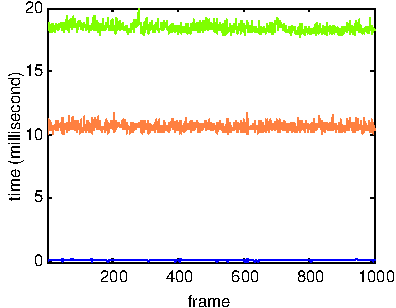
\includegraphics[width=0.49\linewidth]{figs/2/comparison/cupspoon-crop.pdf}}  \hspace{0.05em}
  \subfloat[$\PDg$: rings (Bullet)]{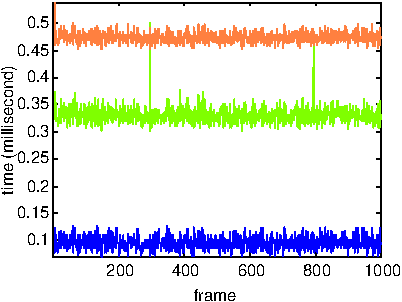
\includegraphics[width=0.49\linewidth]{figs/2/comparison/ring-crop.pdf}}
  \caption[Relative performance of PD computation for different benchmarks]{Relative performance of PD computation for different benchmarks: The blue curve represents the query time computed by our approximate $\PDg$ algorithm. The green curve corresponds to the query time computed using convex decomposition and local PD between convex pairs. The orange curve represents the $\PDg$ query time computed using point-based approximation~\protect\cite{Lien:2009:ASM}.}\label{fig:2:performancecomparison}
\end{figure}



\begin{figure}[!htb]
  \centering
  \subfloat[]{\includegraphics[width=0.49\linewidth, page=4]{figs/2/comparison/PD_bunny_bunny.pdf}}
  \subfloat[]{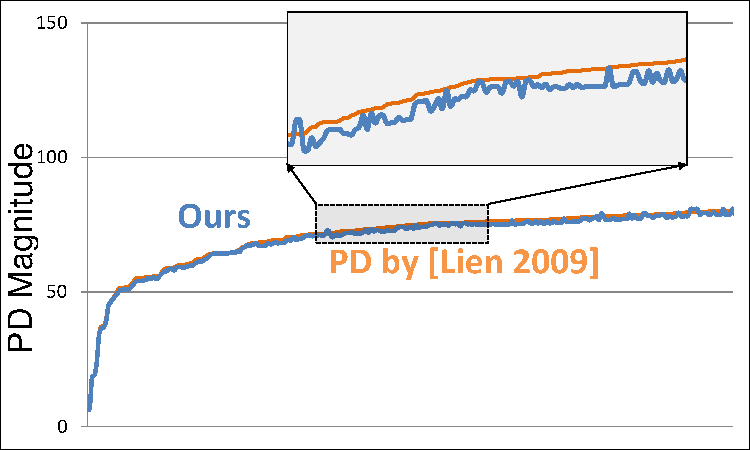
\includegraphics[width=0.49\linewidth, page=1]{figs/2/comparison/PD_bunny_bunny.pdf}}\\
  \subfloat[]{\includegraphics[width=0.49\linewidth, page=2]{figs/2/comparison/PD_bunny_bunny.pdf}}
  \subfloat[]{\includegraphics[width=0.49\linewidth, page=3]{figs/2/comparison/PD_bunny_bunny.pdf}}
  \caption[The performance and accuracy compared to PolyDepth on bunny-bunny benchmark]{The performance and accuracy compared to PolyDepth~\protect\cite{Je:2012:PRP} on the bunny-bunny benchmark. (a) computational time (on average, 0.10ms based on our algorithm vs. 7.15ms in PolyDepth); (b) accuracy comparison between our interactive algorithm vs. an offline algorithm based on Minkowski sum~\protect\cite{Lien:2009:ASM}; (c) accuracy comparison of PD computation between our algorithm vs. PolyDepth; (d) our global PD algorithm (blue) has lower error compared to PolyDepth, which performs local optimization. }\label{fig:2:bunnymodels}
\end{figure}

\begin{figure}[!htb]
  \centering
  \subfloat[]{\includegraphics[width=0.49\linewidth, page=4]{figs/2/comparison/PD_dragon_dragon.pdf}}
  \subfloat[]{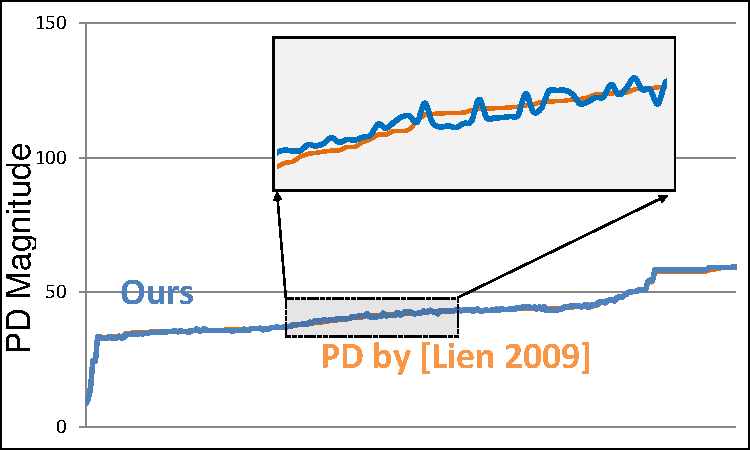
\includegraphics[width=0.49\linewidth, page=1]{figs/2/comparison/PD_dragon_dragon.pdf}}\\
  \subfloat[]{\includegraphics[width=0.49\linewidth, page=2]{figs/2/comparison/PD_dragon_dragon.pdf}}
  \subfloat[]{\includegraphics[width=0.49\linewidth, page=3]{figs/2/comparison/PD_dragon_dragon.pdf}}
  \caption[The performance and accuracy compared to PolyDepth on dragon-dragon benchmark]{The performance and accuracy compared to PolyDepth~\protect\cite{Je:2012:PRP} on the dragon-dragon benchmark. (a) computational time (on average, 0.12ms based on our algorithm vs. 9.86ms in PolyDepth); (b) accuracy comparison between our interactive algorithm vs. an offline algorithm based on Minkowski sum~\protect\cite{Lien:2009:ASM}; (c) accuracy comparison of PD computation between our algorithm vs. PolyDepth; (d) our global PD algorithm (blue) has lower error compared to PolyDepth, which performs local optimization.}\label{fig:2:dragonmodels}
\end{figure}

In order to evaluate the error in our approximate PD computation algorithm, we need to compute the ground truth for the PD value between two objects. For translational PD, the ground truth PD can be obtained by computing the Minkowski sum between two objects. 
It is difficult to compute exact Minkowski sum for complex 3D objects like the teeth or dragon, due to the combinatorial complexity arises. Instead we use the point-based algorithm~\cite{Lien:2009:ASM} to approximate the PD value and estimate the error of our algorithm.
For generalized PD, the ground truth PD computation is even harder. Therefore, we approximate the exact contact space with many slices of Minkowski sums. Intuitively, we sample many rotations in $\SOcubic$ and then compute Minkowski sums for all the rotations. The combination of these Minkowski sums is used as an approximation to the contact space. We label the PD computed using these offline techniques as "\emph{nearly exact PD}" for our algorithm and comparisons.
In practice, our approach is more than an order of magnitude faster than other algorithms that are based on convex decomposition (e.g., \cite{Kim:2002:FPD} for $\PDt$; \cite{Zhang:2007:GPD} for $\PDg$) or point-based approximations. We have compared the runtime performance of our algorithm with these prior global methods in Figure~\ref{fig:2:performancecomparison}. 


\subsection{Comparison with Prior Methods}
Many existing algorithms perform local analysis of intersection regions and
compute local PD. Other techniques use distance fields and can be accelerated using GPUs. In practice, these techniques are fast and also handle
deformable models. To the opposite, our global PD algorithm involves preprocessing and is mainly designed for rigid objects.
The performance of our runtime query (about $0.1\sim2$ milliseconds) is comparable to or faster than prior local PD algorithms. The main benefit of our approach over local PD methods is the computation of global
translational and rotational PD, which provides a more reliable measure of separating two overlapping objects.
Other algorithms reduce PD computation to constrained optimization~\cite{Nawratil:2009:GPD,Zhang:2007:AFP,Je:2012:PRP,Tang:IGP:2013}.
In these techniques, a sequence of configuration samples on the contact space are iteratively
computed until a local minimum configuration is found. The
performance of these algorithms heavily relies on the initial guess of the local optimization, and it is hard to provide
error bounds in terms of global PD (see Figure~\ref{fig:2:bunnymodels} and~\ref{fig:2:dragonmodels}). 
However, compared to our method, these optimization-based algorithms have several advantages. First, they require no pre-computation and can be applied to environments with many obstacles. Our method's dependence on pre-computation limits its application.
Moreover, if suitable initial guesses are chosen for local optimization, optimization-based PD algorithms such as~\cite{Tang:IGP:2013} may provide better results than our method on generalized PD computation involving rotations, especially for queries with small penetration depths.
This is due to some issues of our approach related to the use of sampling-based approaches and the design of configuration space metrics (more details in Section~\ref{sec:2:discussion}).

Existing algorithms either locally analyze intersection regions or use distance fields to compute local PD. In practice, these techniques are computationally efficient and are capable of handling deformable models but only compute local PD. In contrast, our global PD algorithm computes global translational and rotational PD, which provides a more reliable measure of separating two overlapping objects. It should be noted that our algorithm requires preprocessing and is mainly designed for rigid objects. The performance of our runtime query (about $0.1\sim2$ milliseconds) is comparable to or faster than prior local PD algorithms. Other algorithms reduce PD computation to constrained optimization~\cite{Nawratil:2009:GPD,Zhang:2007:AFP,Je:2012:PRP,Tang:IGP:2013} in which a sequence of configuration samples on the contact space are iteratively computed until a local minimum configuration is found. The performance of these algorithms heavily relies on the initial guess of the local optimization, and it is hard to provide error bounds in terms of global PD (see Figure~\ref{fig:2:bunnymodels} and~\ref{fig:2:dragonmodels}). These techniques require no pre-computation and can be applied to environments with many obstacles but the solution heavily depends on the initial guess. If suitable initial guesses are chosen, optimization-based PD algorithms such as~\cite{Tang:IGP:2013} may provide better results than our method on generalized PD computation involving rotations, especially for queries with small penetration depths. This is due to some issues of our approach related to the use of sampling-based approaches and the design of configuration space metrics (more details in Section~\ref{sec:2:discussion}).

\subsection{Implementation Issues}

\paragraph{Collision Checking}
Our method is able to correctly compute the contact space for complex non-convex and non-manifold models assuming that a `correct' collision detection routine is available for input geometric data; the `correctness' means that the collision result provided by the collision checking routine can correctly reflect objects' collision status in physical world. In our implementation, we used the OBBTree algorithm~\cite{Gottschalk:1996:OHS} for collision checking between objects represented as mesh soups. Since mesh soups lack connectivity information between mesh triangles, the above assumption may not hold in some degenerate cases. For instance, if two objects are so different in scale that one object $A$ can be completely contained inside the other object $B$, the collision checking algorithm will always report collision-free for configurations in which $A$ locates inside $B$, while in physical world $A$ and $B$ should be in-collision. Thus, our learning framework will not provide a correct contact space in this case. In addition, when the mesh representation of the object $B$ has a hole larger than the size of the object $A$ (Figure~\ref{fig:2:hole}), the collision checking routine will also give incorrect results. To handle these degenerate cases, one possible solution is to use sophisticated collision detection algorithms such as~\cite{Ju:2004:RRP} to recover or estimate objects' volumetric information from mesh soups, and then applying volumetric collision checking between objects.

\begin{figure}[!htb]
  \centering
  \subfloat[]{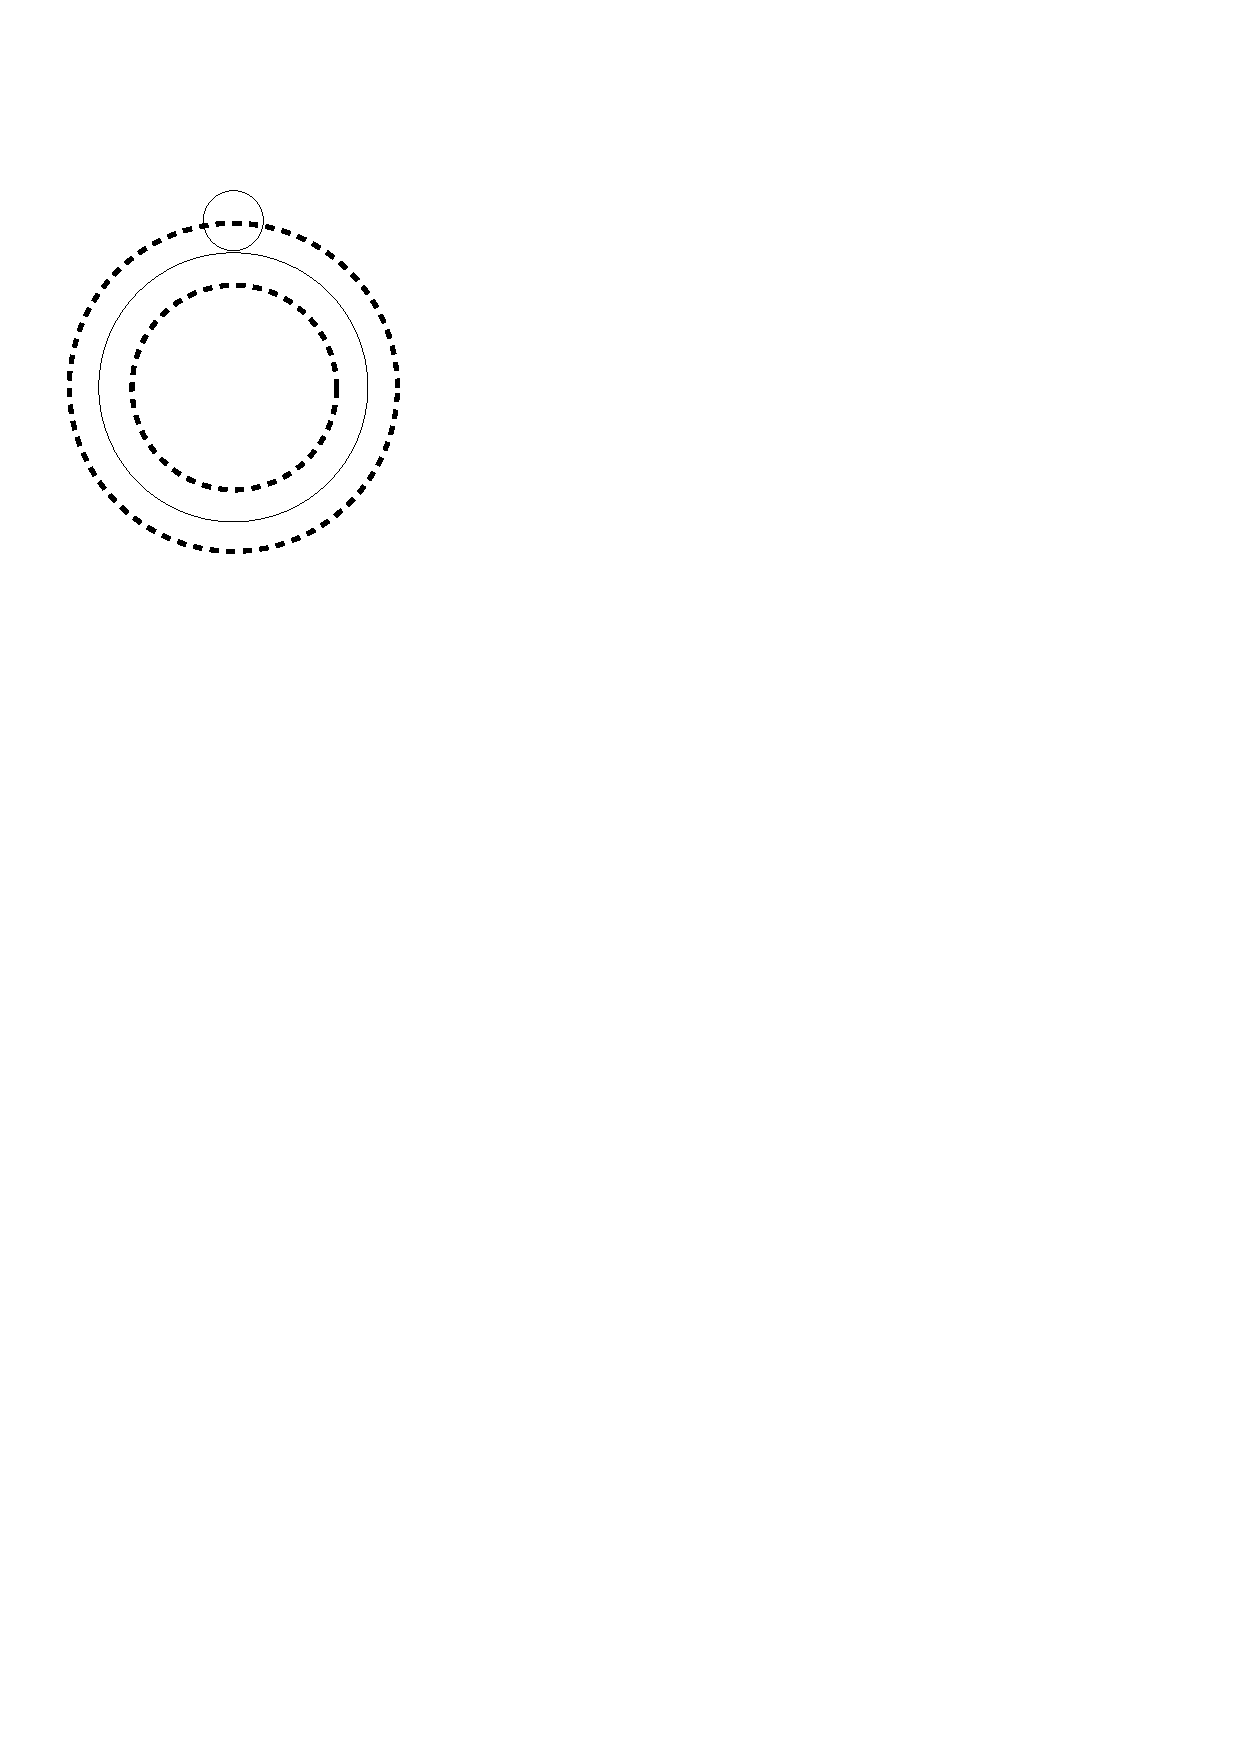
\includegraphics[width=0.3\linewidth]{figs/2/hole1.pdf}}
  \subfloat[]{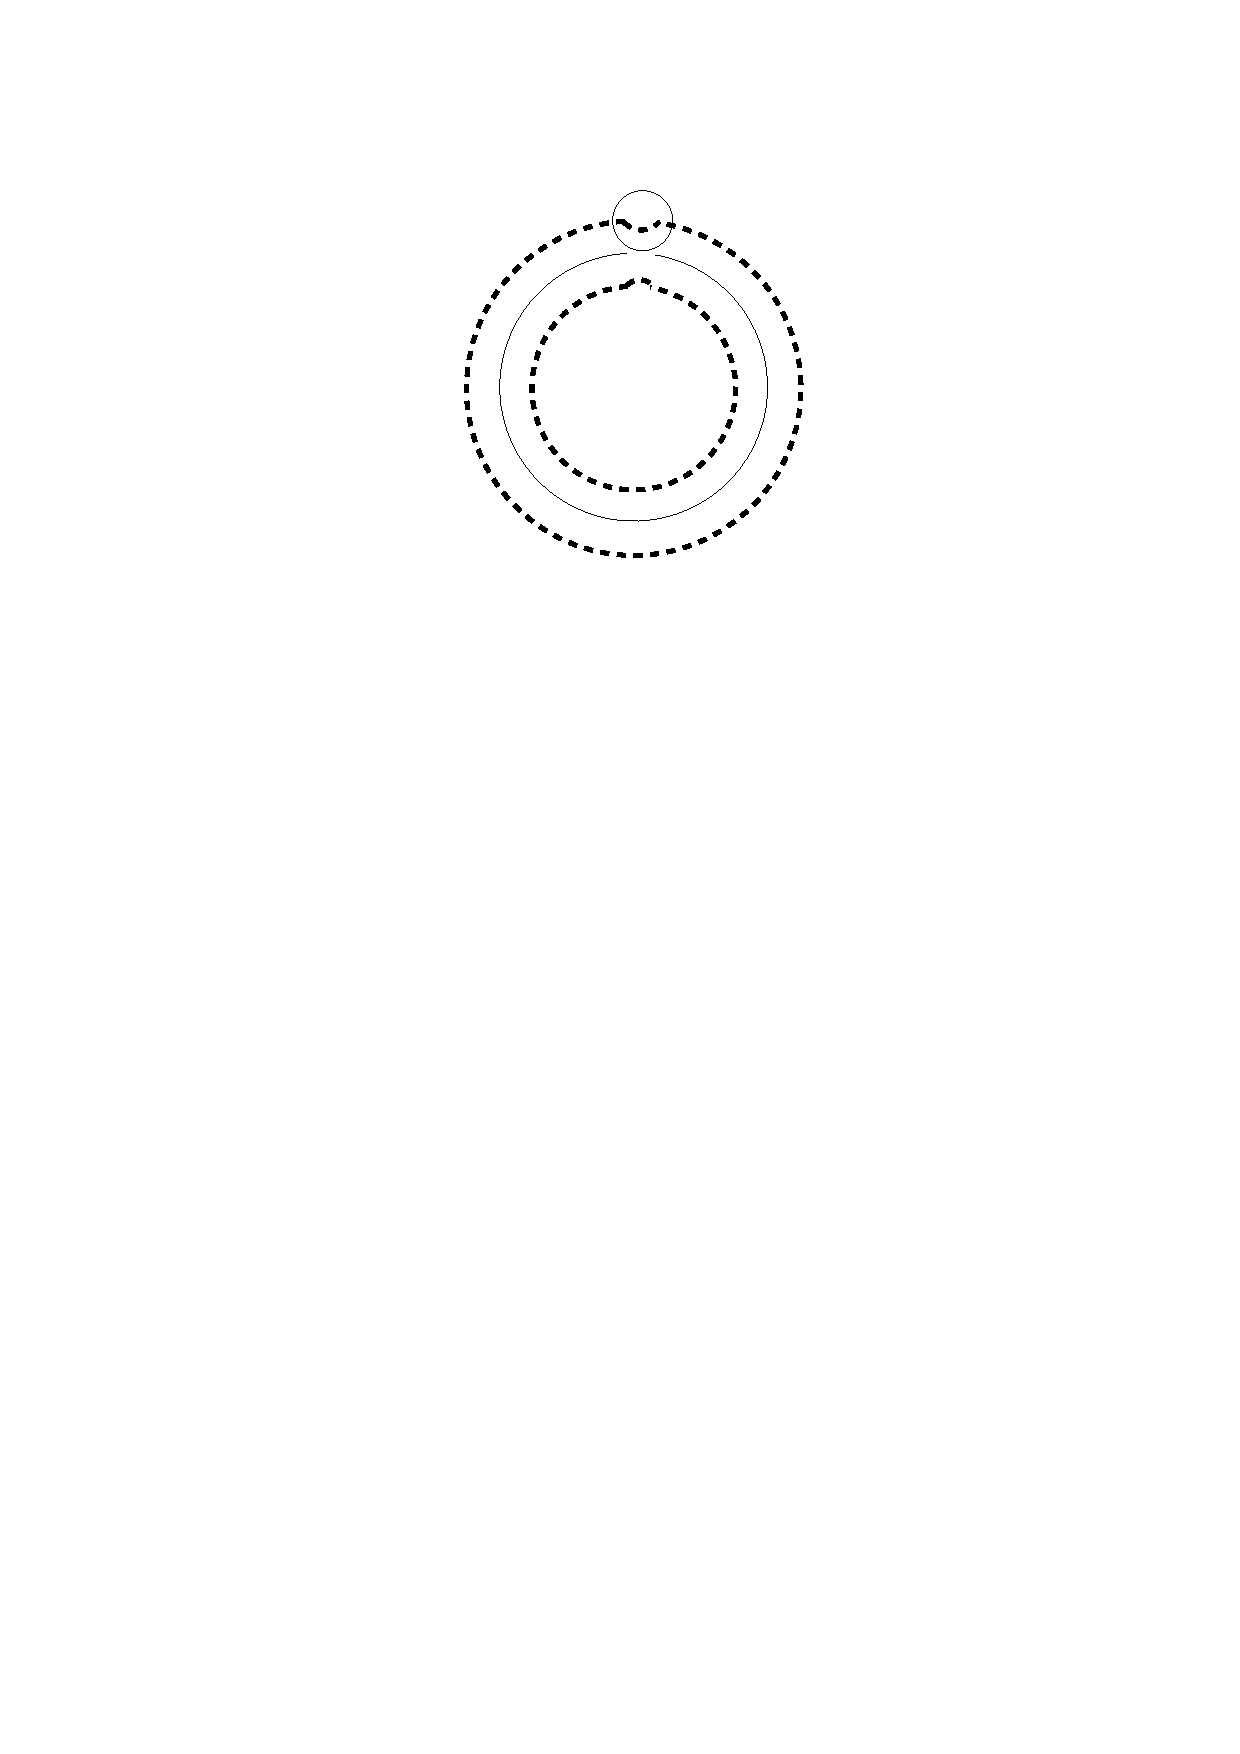
\includegraphics[width=0.3\linewidth]{figs/2/hole2.pdf}}
  \subfloat[]{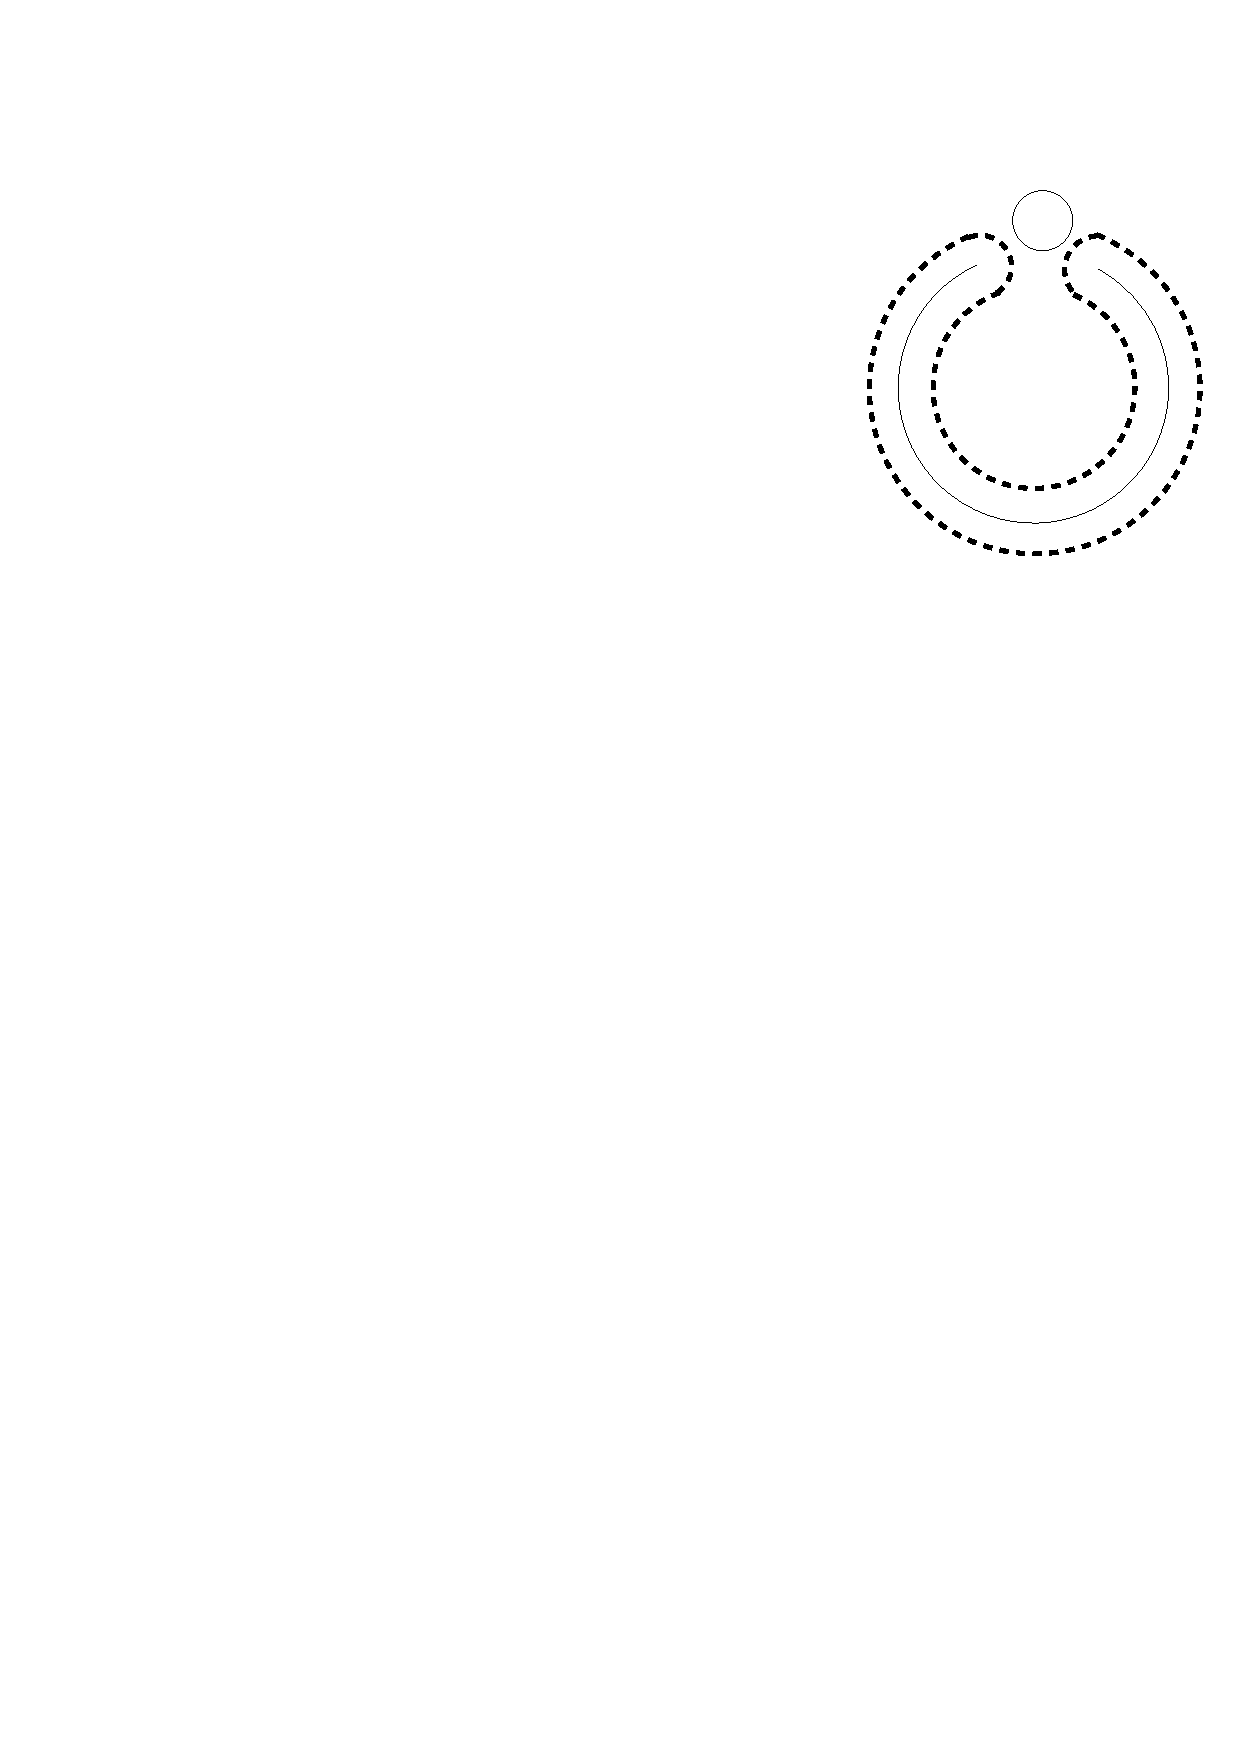
\includegraphics[width=0.3\linewidth]{figs/2/hole3.pdf}}
  \caption[One example for the degenerate case of configuration space approximation]{One example for the degenerate case of configuration space approximation.
We are given two objects: one large circle and one small circle. (a) When the geometric representations of both objects are exact, the contact space can be illustrated as dashed circles. (b) When the big circle has a small hole, the contact space (the dashed curves) is slightly different with the exact contact space in (a). (c) If the big circle has a large hole, the contact space (the dashed curve) is topologically different with the exact contact space in (a). In many applications, the geometric representation of objects have hole artifacts, which may result in low quality contact spaces similar to (c). 
}\label{fig:2:hole}
\end{figure}


\paragraph{SVM Implementation}
We use the hard-margin SVM (Equation~\ref{eq:2:svm1}) in Section~\ref{sec:2:offline:svm} to introduce the main concept underlying our learning framework, since all in-collision samples and collision-free samples are separable. However, we use a soft-margin SVM in our implementation, which is defined as follows:
\begin{align}
\label{eq:2:svmsoft}
& \underset{\mathbf w, b, \xi}{\text{min}} & & \frac{1}{2}\|\mathbf w\|^2 + C \sum_{i=1}^k \xi_i & &  \\
& \text{subject to} & & c_i (\mathbf w \cdot \phi(\mathbf q_i) + b)
\geq 1 - \xi_i, & & \xi_i \geq 0 & & 1 \leq i \leq k. \notag
\end{align}
Here, slack variables $\xi_i$ measure the degree of misclassification of the data; the objective function is increased by a term which uses a weight variable $C$ to penalize non-zero $\xi_i$. The optimization becomes a trade-off between a large margin and a small error penalty. 

In practice, a soft-margin SVM behaves better than a hard-margin SVM, even when data is separable. The reason is that for a hard-margin SVM, a single outlier (e.g., a sample extremely close to the actual contact space) can determine the boundary, which makes the classifier overly sensitive to the data. For contact space learning, a hard-margin SVM will generate an uneven contact space with jagged edges, while a soft-margin SVM can provide a smooth contact space. 

However, the soft-margin SVM needs to select an appropriate penalty weight $C$, which is not an easy task. A suitable value of $C$ is related to the set of samples used to learn a contact space; it is also related to the number of samples used. A small value of $C$ will result in a large error in the approximate contact space, while a large $C$ will result in a non-smooth contact space or a contact space approximation with an incorrect topology. Theoretically, cross-validation provides a systematic manner for choosing $C$, but it is computationally expensive. In our experiments, we run the learning algorithms with different $C$ values and then choose the $C$ generating an approximate configuration space with the smallest error. 


\paragraph{Learning on Non-Euclidean Structure}
Our algorithm attempts to compute a global representation for the contact space, i.e., a representation that is valid and accurate for any points in the contact space. An accurate global representation is challenging in the case of non-Euclidean spaces such as $\SEcubic$ because it is difficult to have an Euclidean space globally approximate a non-Euclidean space while also preserving the considered distance metric. However, it is possible to provide a Euclidean approximation with high accuracy to a non-Euclidean space locally around a configuration. This approximation strategy is widely used in optimization-based local PD algorithms such as~\cite{Nawratil:2009:GPD,Zhang:2007:AFP,Je:2012:PRP,Tang:IGP:2013}, in which different heuristics have been proposed to approximate the contact space locally around an in-contact configuration. The local approximation of the contact space is easier to compute than the global contact space. However, a global contact space is only computed once during the pre-computation step and can be reused during online PD queries. In other words, our method attempts to solve a more challenging problem than prior methods.

When learning the structure of the contact space in the $\SEcubic$ configuration space, we convert every configuration into a vector in the Euclidean space: for the rotation component of each configuration, we either convert it into a $3$-dimensional vector corresponding to the Euler angles, or into a $4$-dimensional vector corresponding to a quaternion. Given the vector representation of each configuration, we then perform the learning algorithm directly in the Euclidean space. However, $\SEcubic$ in fact is a Lie group and the Euclidean space approximation is only valid locally around each configuration. More formally, the Euclidean space locally approximates the Lie algebra element $\exp(\mathbf q)$ of a given configuration $\mathbf q \in \SEcubic$, where $\exp$ is the exponential map from $\SEcubic$ to its corresponding Lie algebra $\mathfrak{se}(3)$~\cite{Murray:1994:MIR}. This assumption might not hold for computing contact spaces with significant rotation components. In order to learn the non-Euclidean contact space precisely, one possible solution is to directly use learning algorithms on Lie groups~\cite{Tuzel:2008:LLG}.

\section{Discussion: Discrete Sampling, $\Cspace$ Metrics and Optimization Techniques}
\label{sec:2:discussion}

There are three main factors that influence the accuracy of penetration depth values computed by our approach: discrete sampling, $\Cspace$ metrics, and the choice of optimization technique. Since these three factors are closely related to each other, we first discuss each factor in isolation and then use examples to show how a combination of these factors influences the $\PDg$ computation. 

\paragraph{Discrete Sampling} Our approach performs discrete sampling in the configuration space and uses the generated samples to approximate the contact space, which are then used for computing penetration depth values. The accuracy of the contact space improves with an increase in the number of samples (Figure~\ref{fig:2:activelearningtime}). Since we formulate penetration depth as an optimization problem on the approximate contact space, a larger number of samples also improves the accuracy of the penetration depth computation, as we will show later in Figure~\ref{fig:2:samplenumber}. However, due to the curse-of-dimensionality, it is challenging to generate a sufficient number of samples in higher-dimensional configuration spaces. This explains why, given the same number of samples, the $\PDt$ accuracy on $\SEcubic$ is worse than the $\PDt$ accuracy on $\Rcubic$.

\paragraph{$\Cspace$ Metric} The penetration depth formulation in Equation~\ref{eq:2:PDgdef} requires a suitable metric to be defined over the entire configuration space, which correctly measures the distance between any two points in the configuration space. For $\PDt$, we use the Euclidean metric since the underlying configuration space is Euclidean. However, for $\PDg$, the configuration space is non-Euclidean and hence the metric selection is more challenging. For a specific application, defining a good metric in $\SEcubic$ is a challenge when applying our learning-based framework. We currently use the object norm metric~\cite{Kazerounian:ASME:1992} defined in Equation~\ref{eq:PDgmetric}, which uses weights $\mu_1$, $\mu_2$ and $\mu_3$ to balance the relative weight between the rotational and the translational components. 

The choice of metric is also closely related to the issue of discrete sampling. During the off-line learning phase, we generate a finite number of samples in the configuration space; these samples are used to compute the approximate configuration space. During runtime, a given in-collision query $\mathbf q_0$ is projected onto the set of these discrete samples via global optimization (i.e., the nearest-neighbor algorithm), to obtain the corresponding in-contact configuration $\mathbf q_c$. Large $\mu_i, i=\{1,2,3\}$ values imply a large penalty to configurations' difference in the rotational component. Theoretically, we can use $\PDg$ to compute $\PDt$ when $\mu_i \rightarrow \infty, i=\{1,2,3\}$, but this is infeasible in practice due to the use of sampling-based techniques. Among all the pre-computed samples in the configuration space, there may be no samples with the same rotational component as the query configuration $\mathbf q_0$. Thus, our sampling-based framework can only provide an in-contact configuration whose rotational component is close to that of $\mathbf q_0$, which may result in incorrect PD value computation.

The selection of $\mu_i$ values in the metric formulation will greatly influence the final PD values. Large $\mu_i$ values may also result in high ``vibrations'' in the PD values, especially when the moving object is rotating. This is because the $\mu_i$ values are the derivatives of the metric function with respect to the rotational component, and thus large $\mu_i$ values will make the nearest-neighbor algorithm highly sensitive to the change in the query's rotational component. As a result, a slight rotation of the moving object $A$ will result in a large change in the PD value. Large $\mu_i$ values will also cause other problems. For instance, let us assume that we are given a query configuration with a small penetration. Intuitively, the PD algorithm should return an in-contact sample which has a translational component similar to the query and with an appropriate rotational component. However, due to the limited number of samples for approximating the contact space, it is possible that all the samples closest to the query in translation have a larger rotational difference with the query, than one sample $\mathbf q_{bad}$ that is far away from the query in translation. For large $\mu_i$ values, the difference in the rotational components dominates the distance between the query and other samples, especially for a query with a small penetration. As a result, $\mathbf q_{bad}$ will be the in-contact sample reported by our PD method, even though it is not the desired result. Such inaccuracy is smaller for a query with a deep penetration, because the translational difference comprises a larger component of the PD measurement for queries with deeper penetrations. Similar inaccuracies will arise when the $\mu_i$ values are too small. 

The interaction between the object norm metric and sampling-based techniques also results in the discontinuity of $\PDg$ values. Suppose the moving object is collision-free at the beginning; at the next instance, it is in contact with the obstacles, and finally collides with some obstacles. Intuitively, the PD value should be zero when the contact first occurs and then should increase continuously. However, since there are only a finite number of configuration samples in the approximate contact space, we usually cannot find a sample exactly the same as the in-contact query. Under the object norm metric, the in-contact sample closest to the query always has a non-zero distance to the query, no matter how many samples are generated for approximating the contact space (because the measure of a limited number of samples is zero in the continuous configuration space). As a result, the approximate PD for a given query will suddenly ``jump'' from a zero value to a non-zero value; such jumps may not be acceptable in many applications where high fidelity results are required such as haptics. 

If an infinite number of samples are available, the ``jump'' and vibration problems mentioned above will disappear. In practice, when the number of samples increases, the accuracy of $\PDg$ improves and the magnitude of ``jump'' and vibration decreases, as shown in Figure~\ref{fig:2:samplenumber}.

\begin{figure}[!h]
\centering
  \subfloat[jump]{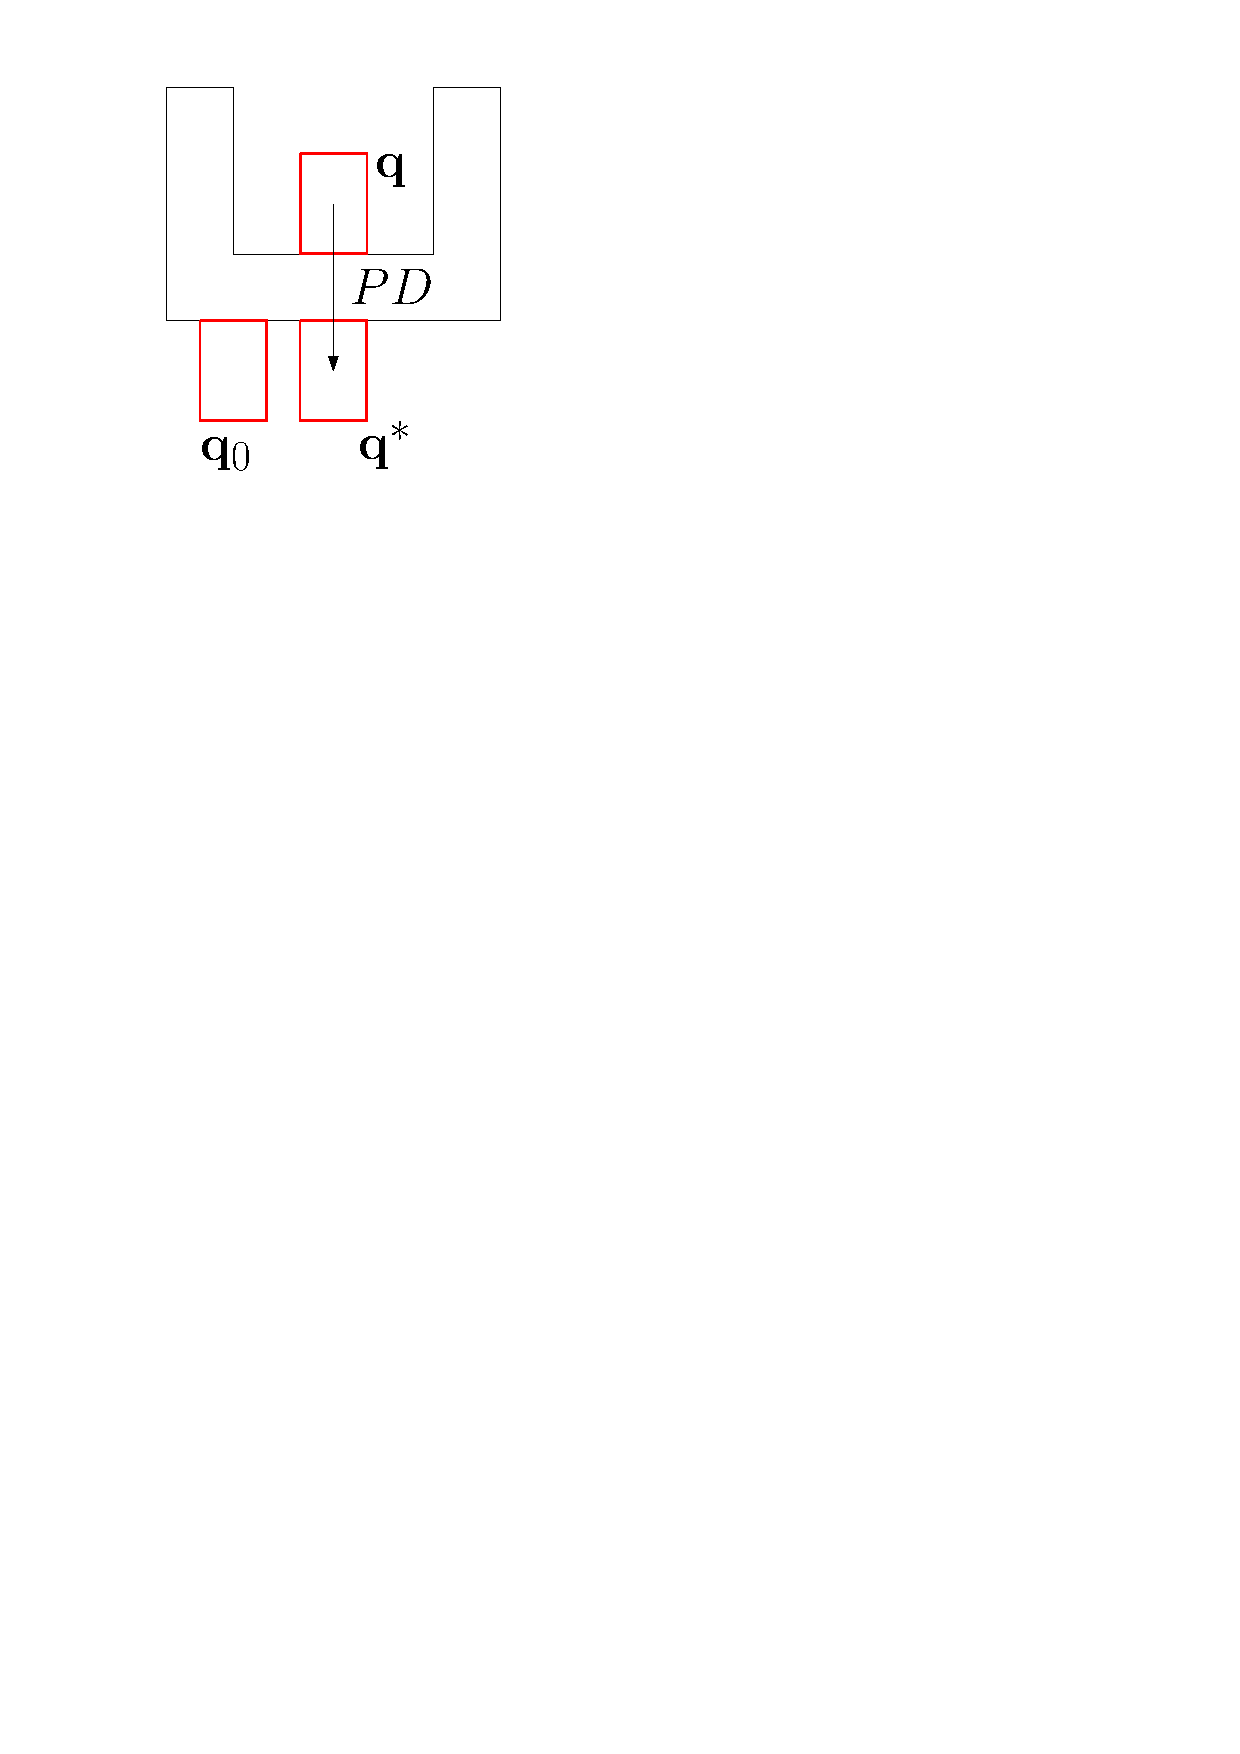
\includegraphics[width=0.3\linewidth]{figs/2/local_jump.pdf}}
  \subfloat[vibration]{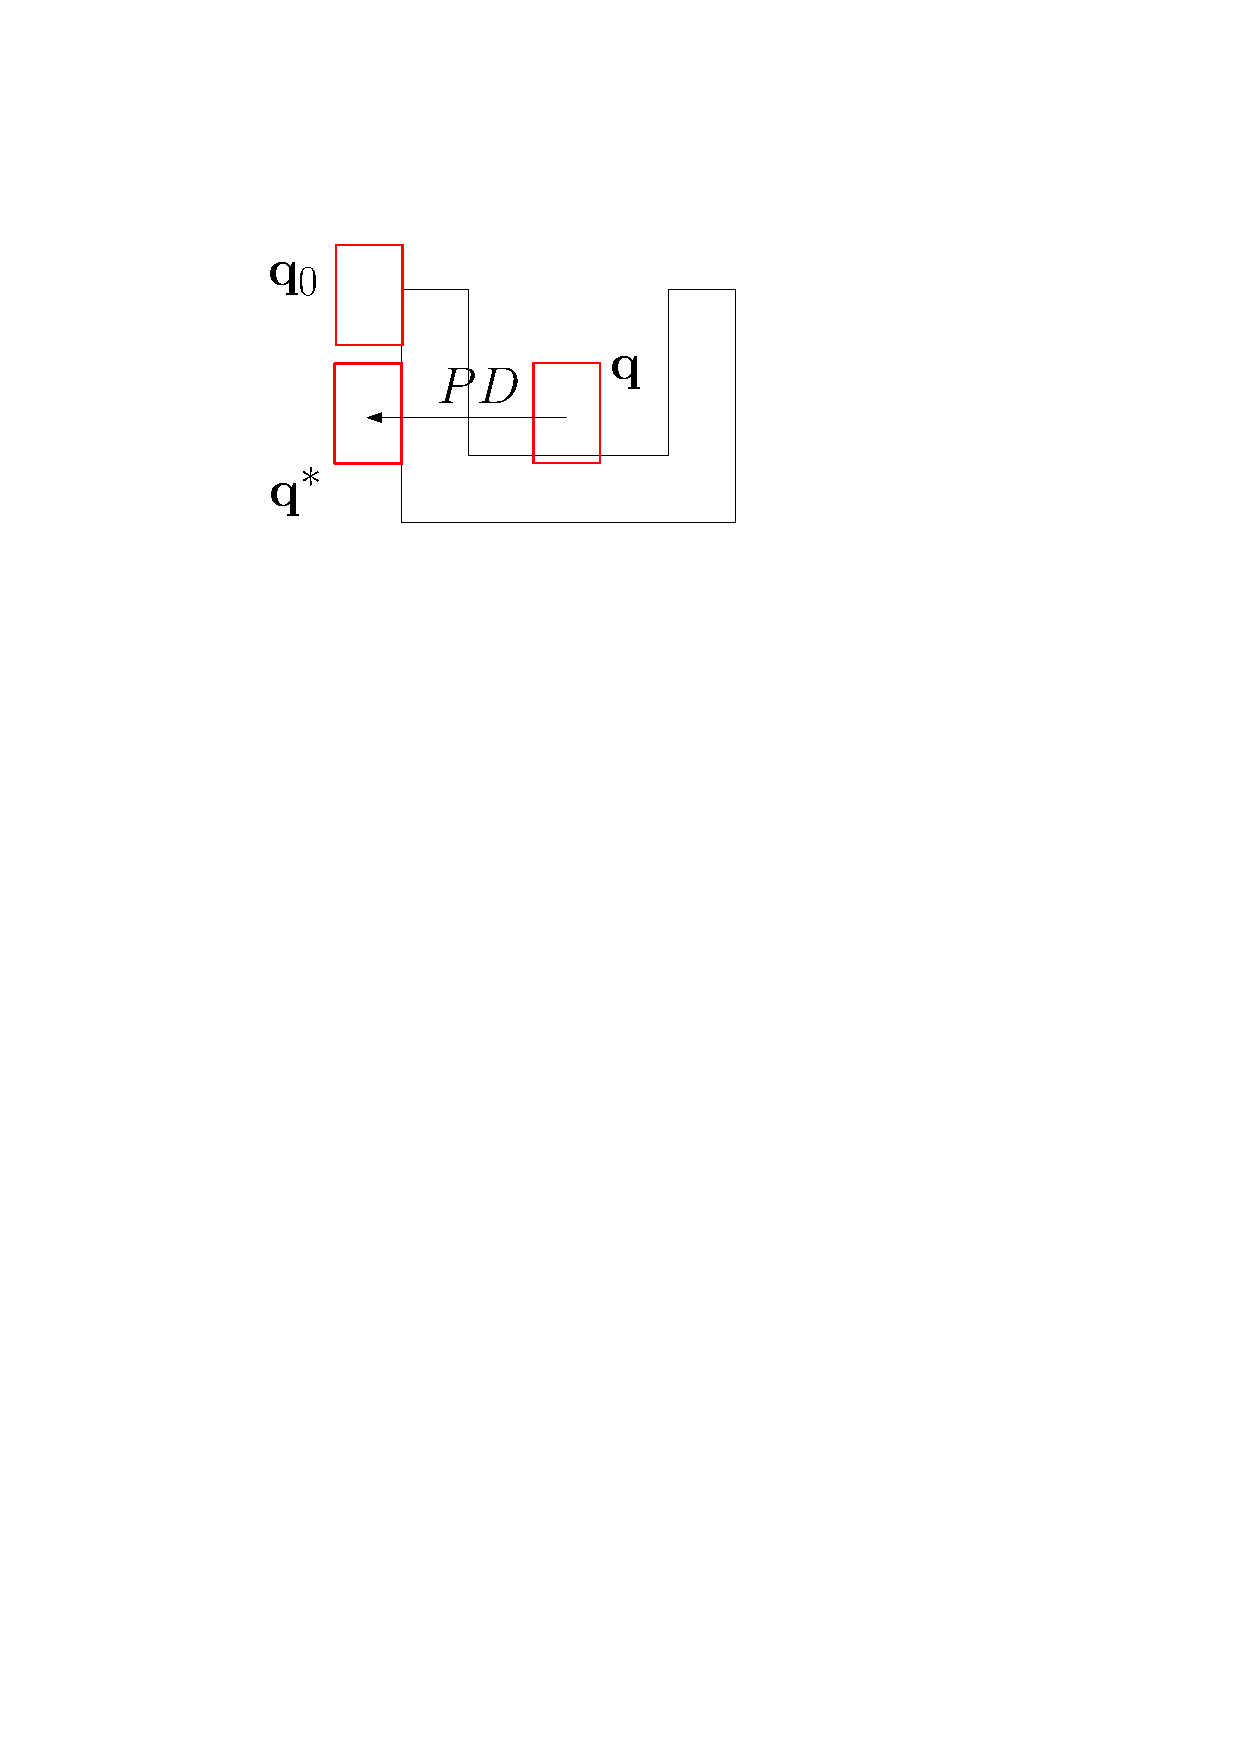
\includegraphics[width=0.45\linewidth]{figs/2/local_vibration.pdf}}
\caption[The ``jump'' and vibration problems when using optimization-based PD algorithms]{The ``jump'' and vibration problems when using optimization-based PD algorithms. The black polygon is the obstacle and the red object is the moving object. (a) Given the in-contact query configuration $\mathbf q$ and the initial guess $\mathbf q_0$, an optimization-based PD algorithm's result would be $\mathbf q^*$. Apparently, $\dist(\mathbf q, \mathbf q^*) \neq 0$ and thus ``jump'' happens. (b) When the query configuration $\mathbf q$ translates slightly compared to (a), the PD value and PD direction may change abruptly. This is because different initial configurations are chosen for the local optimization and thus vibration happens. }\label{fig:2:local_artifact}
\end{figure}


\paragraph{Optimization Techniques} Choosing appropriate optimization techniques is critical for the accuracy of penetration depth computation. Our approach uses a nearest neighbor routine as the optimization algorithm due to its dependence on discrete samples. As discussed above, problems related to configuration space metrics are also closely related to nearest neighbor algorithms. The choice of optimization techniques is also important for optimization-based PD algorithms~\cite{Nawratil:2009:GPD,Zhang:2007:AFP,Je:2012:PRP,Tang:IGP:2013}, which use local optimization on the contact space to find a good penetration depth result. Since the contact space is highly non-convex, the local optimization may be trapped in a bad local minimum if an inappropriate initial configuration is used. Thus, these approaches may also suffer from problems such as discontinuities in PD values and vibrations, as illustrated in Figure~\ref{fig:2:local_artifact}. To alleviate these issues, many heuristics have been proposed in previous optimization-based PD approaches to choose good initial configurations for the local optimization~\cite{Je:2012:PRP,Tang:IGP:2013}.

Our learning-based approach can be combined with optimization-based PD algorithms by using the in-contact configuration computed by our method as the initial guess of optimization-based PD algorithms. In general, such a combination will not solve the discontinuity and vibration problems in PD computation. This is because the in-contact configuration computed by our method may be far away from the global optimal solution and may not be a good initial guess for the local optimizer. Thus, using optimization-based PD algorithms as a post-processing step cannot guarantee to help. 

\begin{figure}[!h]
\centering
\subfloat[Rotation movement]{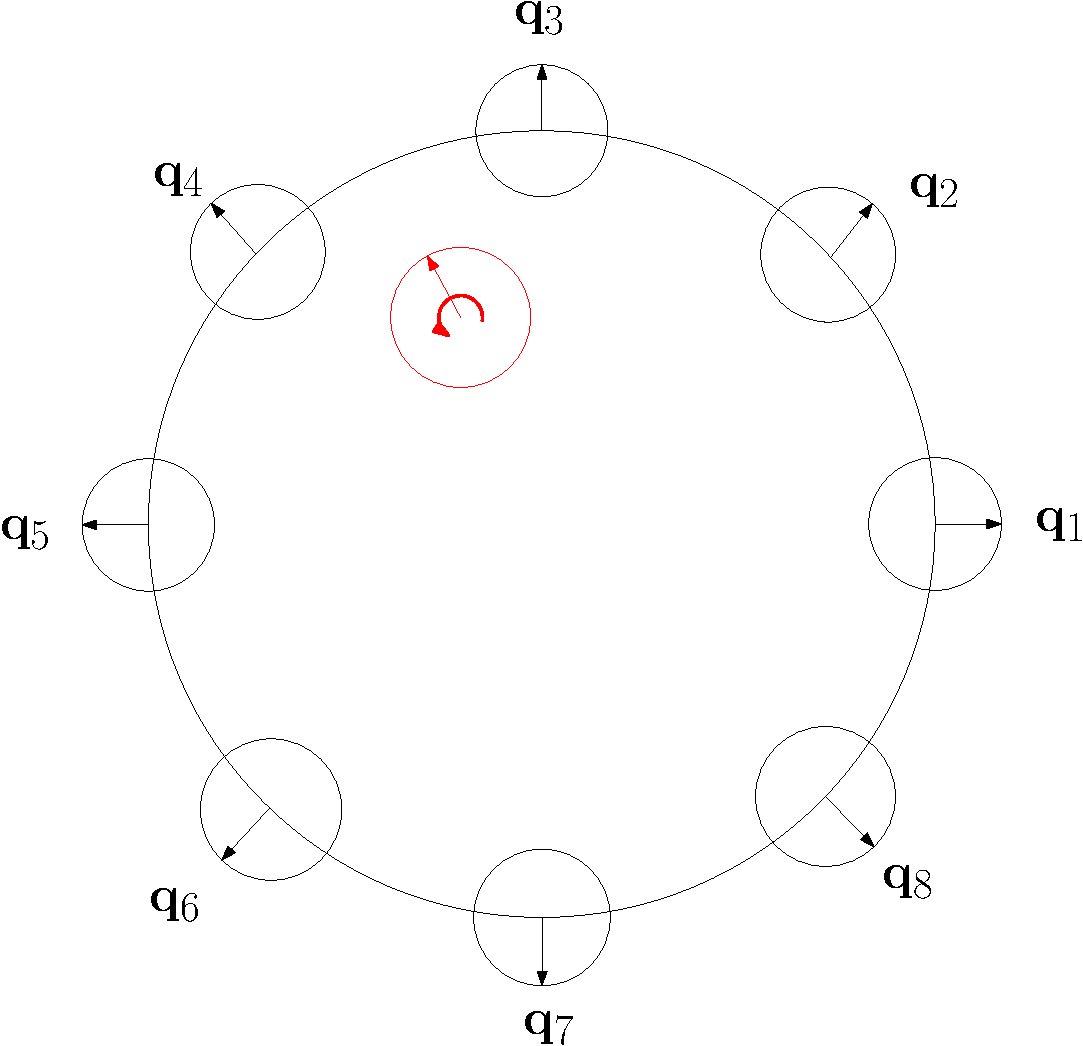
\includegraphics[width=0.48\linewidth]{figs/2/rotation_error.pdf}}
\subfloat[Translational movement]{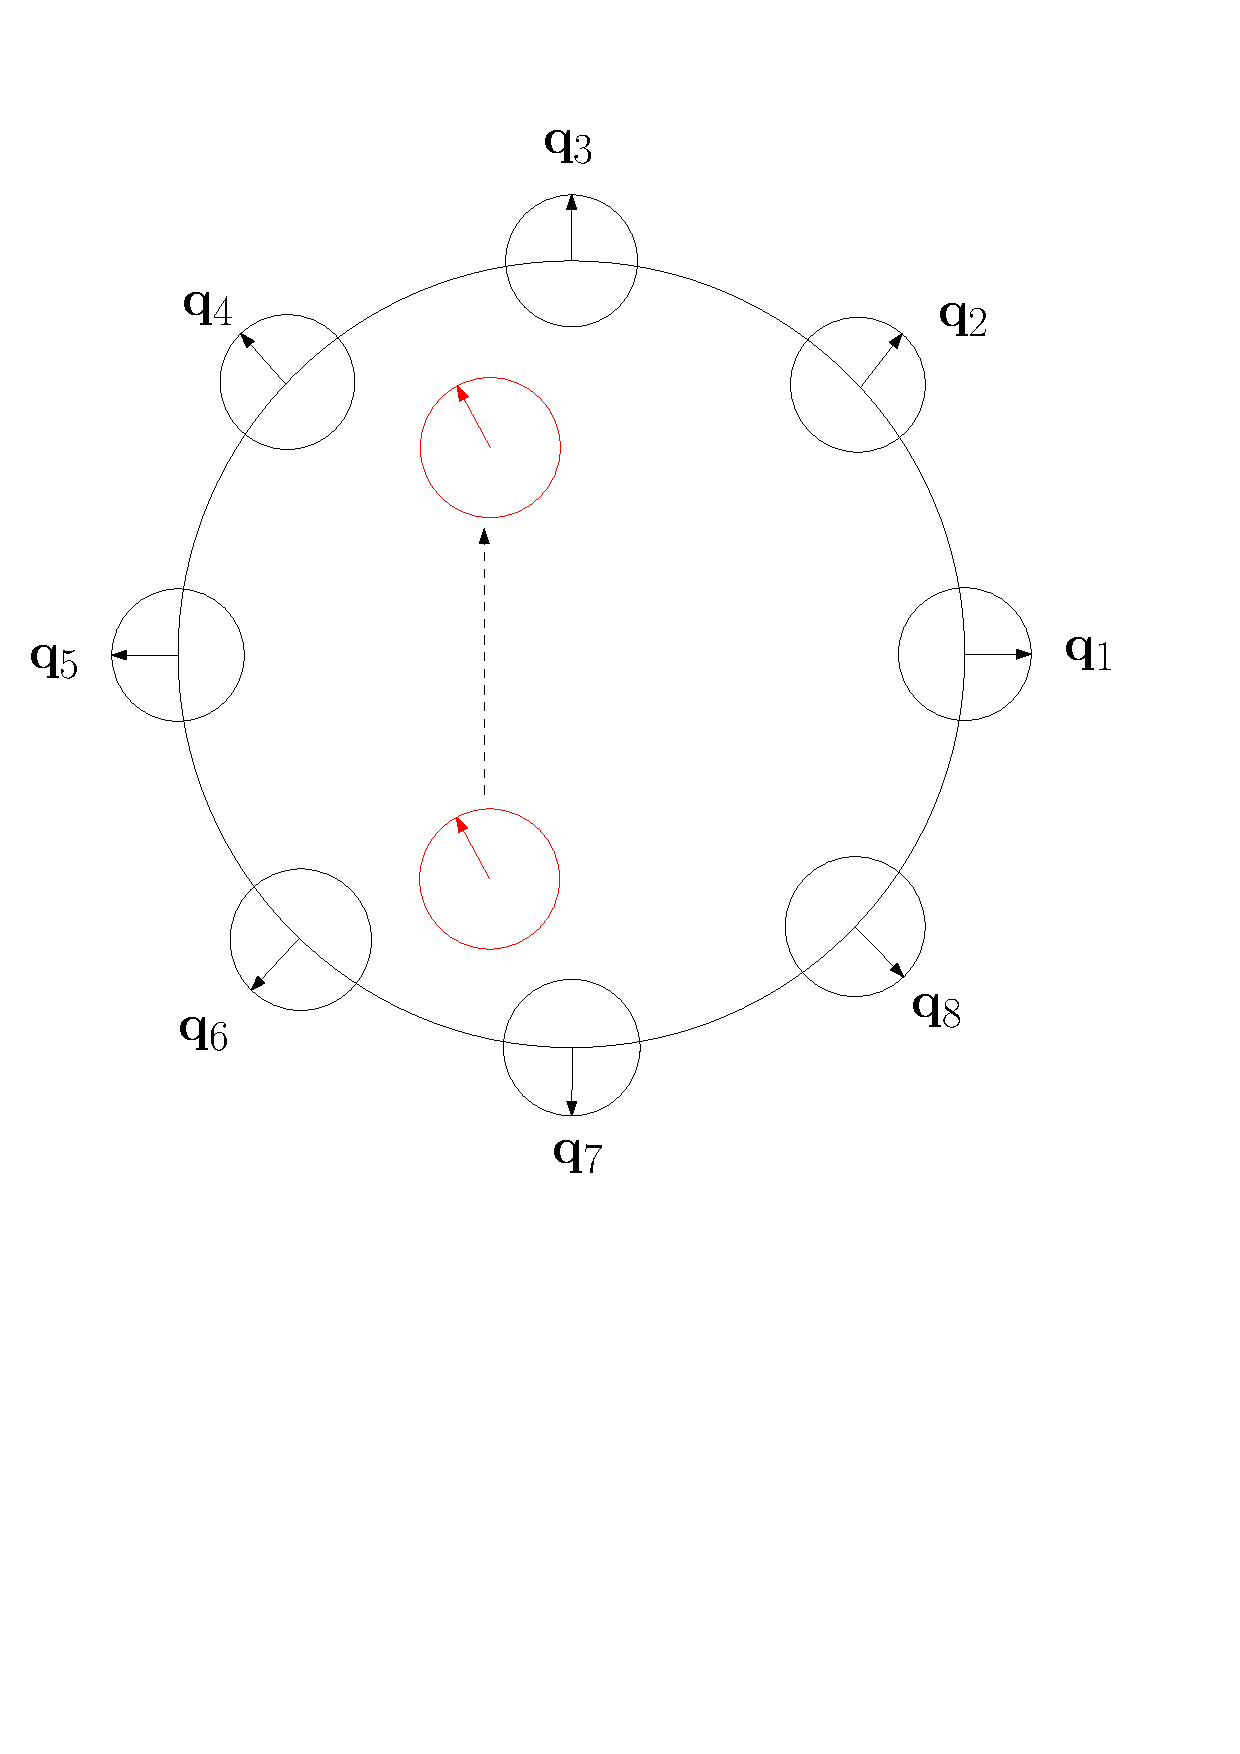
\includegraphics[width=0.48\linewidth]{figs/2/translation_error.pdf}}
\caption[Examples to illustrate how the configuration space metric influences the result of our PD algorithm]{Examples to illustrate how the configuration space metric influences the result of our PD algorithm. The large circle is the $\Cobs$. We use small circles to denote configuration samples in the configuration space: the circle center is the translational component and the arrow's direction indicates the rotational component. We use eight configurations to approximate the contact space. The red circle is the query configuration. In (a), the query rotates counter-clockwise. In (b), the query performs translation motion.}\label{fig:2:toybenchmark}
\end{figure}

To better illustrate the above limitation related to $\SEcubic$ metrics, global optimization and sampling-based techniques, we now use two examples (Figures~\ref{fig:2:toybenchmark}(a) and (b)) to show our $\PDg$ algorithm's behavior under different metric settings. In these examples, we use eight configuration samples to approximate the contact space. The translational components of these configurations are uniformly distributed on a circle with radius $1$; these configurations have rotation angles $\frac{k \pi}{4}$, $k=1,...,8$.

\begin{figure}[!h]
\centering
  \subfloat[$\mu_i = 0$]{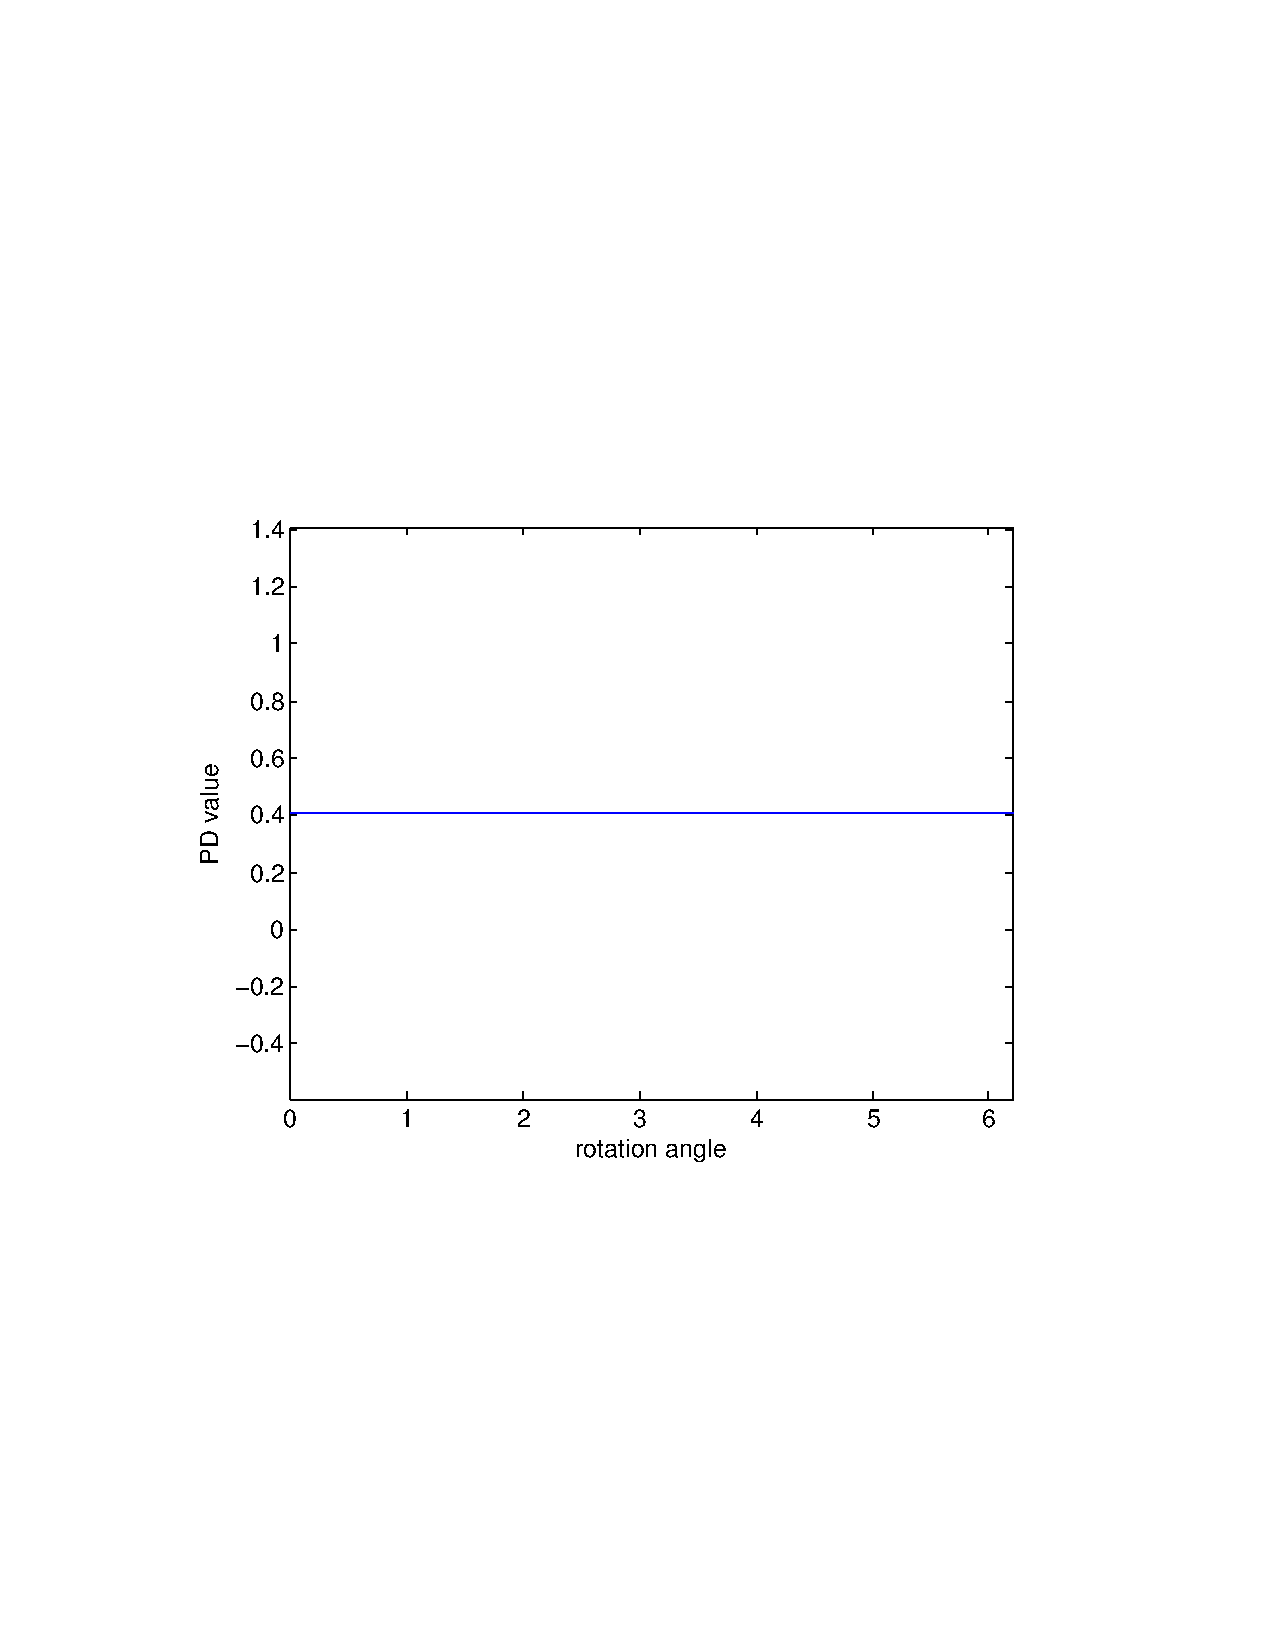
\includegraphics[width=0.33\linewidth, trim=33mm 80mm 40mm 85mm, clip]{figs/2/rotation_error_w00000.pdf}}
  \subfloat[$\mu_i = 0.001$]{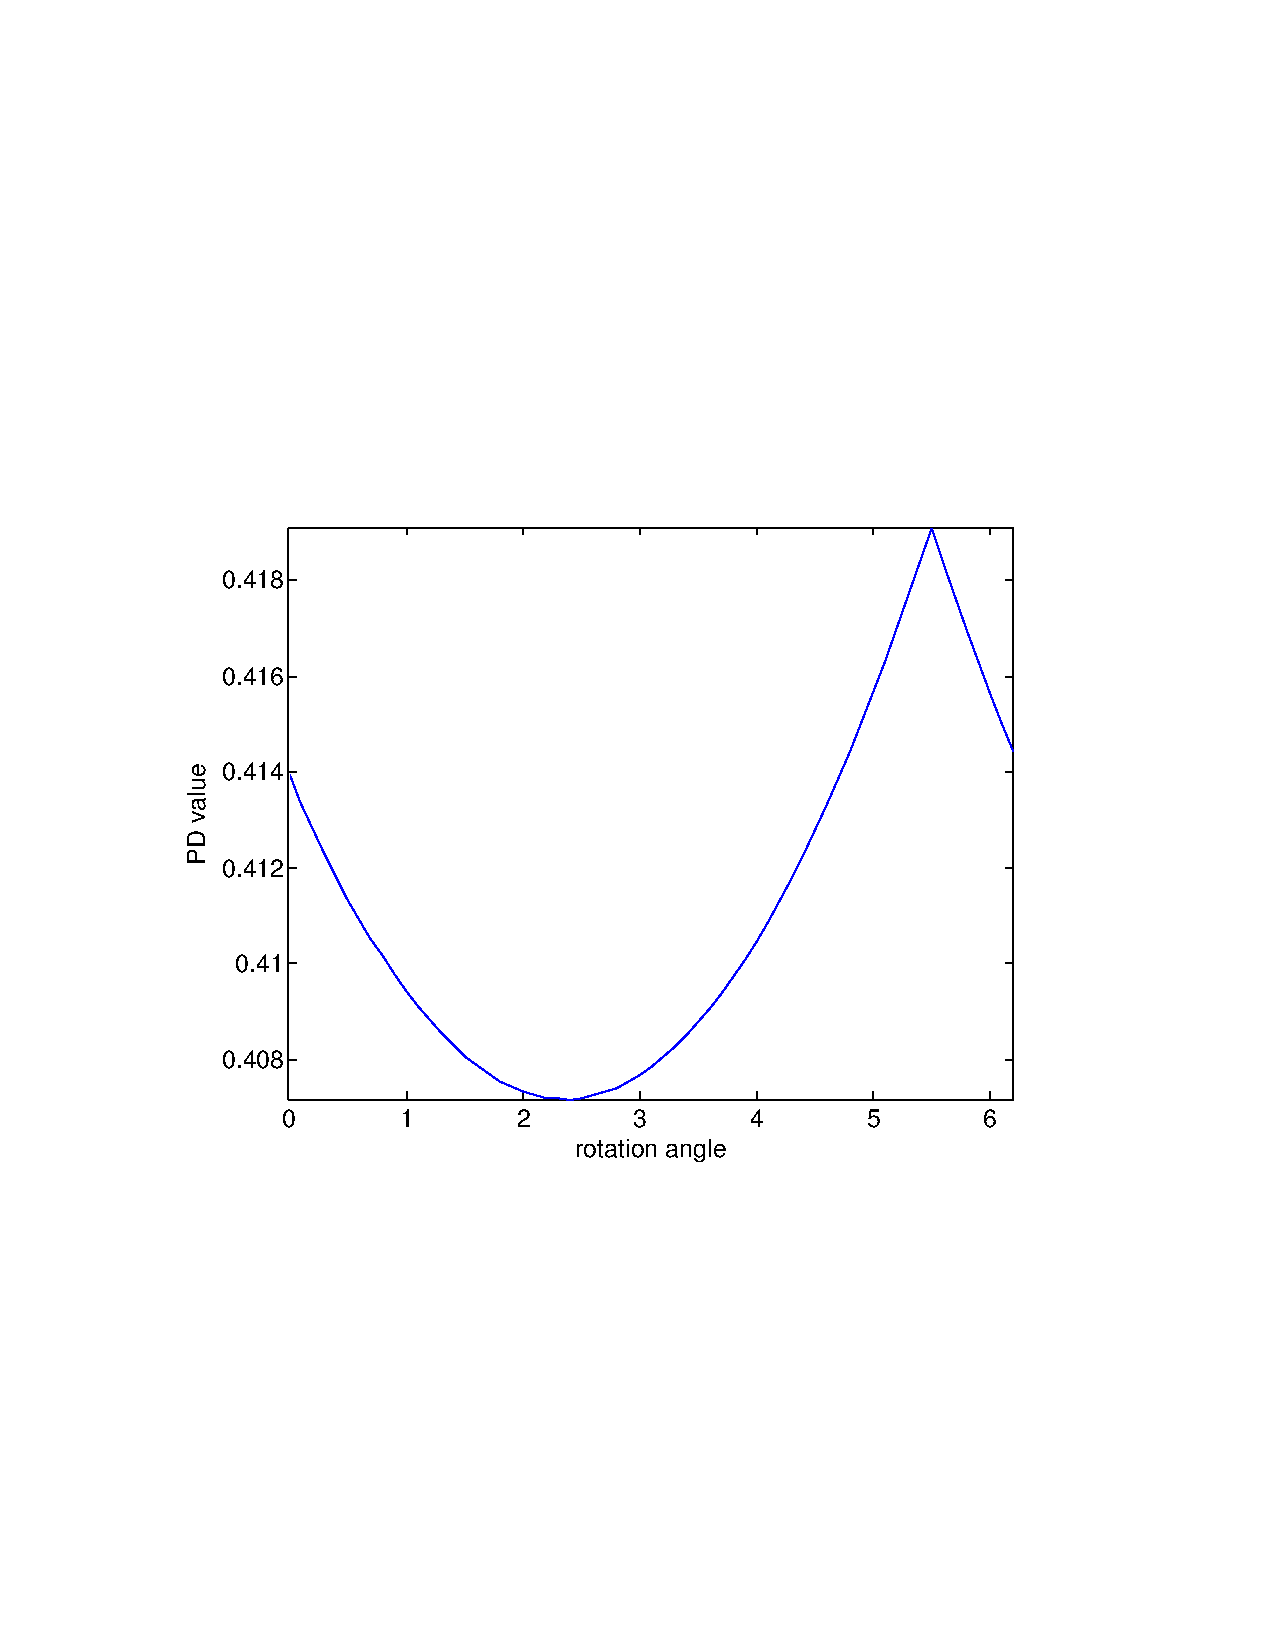
\includegraphics[width=0.33\linewidth, trim=31mm 80mm 40mm 85mm, clip]{figs/2/rotation_error_w0001.pdf}} 
  \subfloat[$\mu_i = 0.01$]{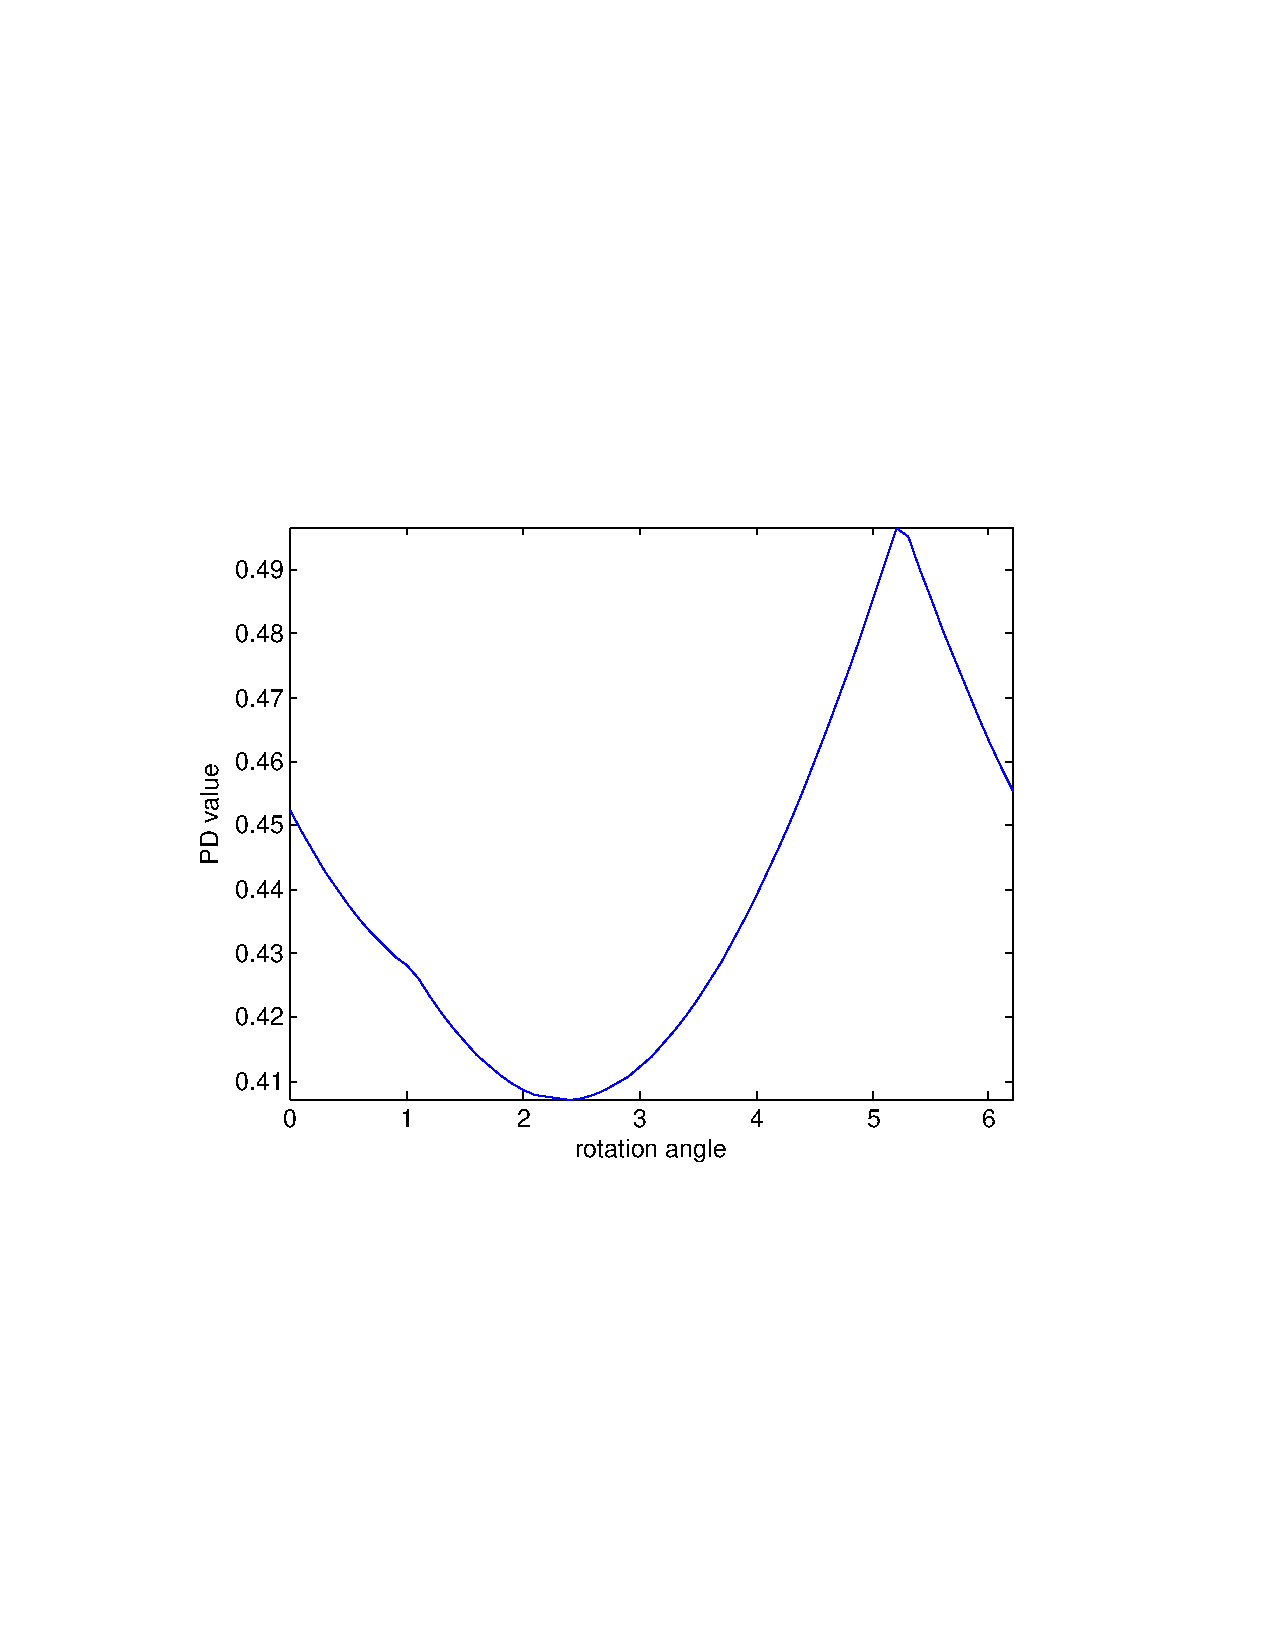
\includegraphics[width=0.33\linewidth, trim=33mm 80mm 40mm 85mm, clip]{figs/2/rotation_error_w001.pdf}} \\
  \subfloat[$\mu_i = 0.1$]{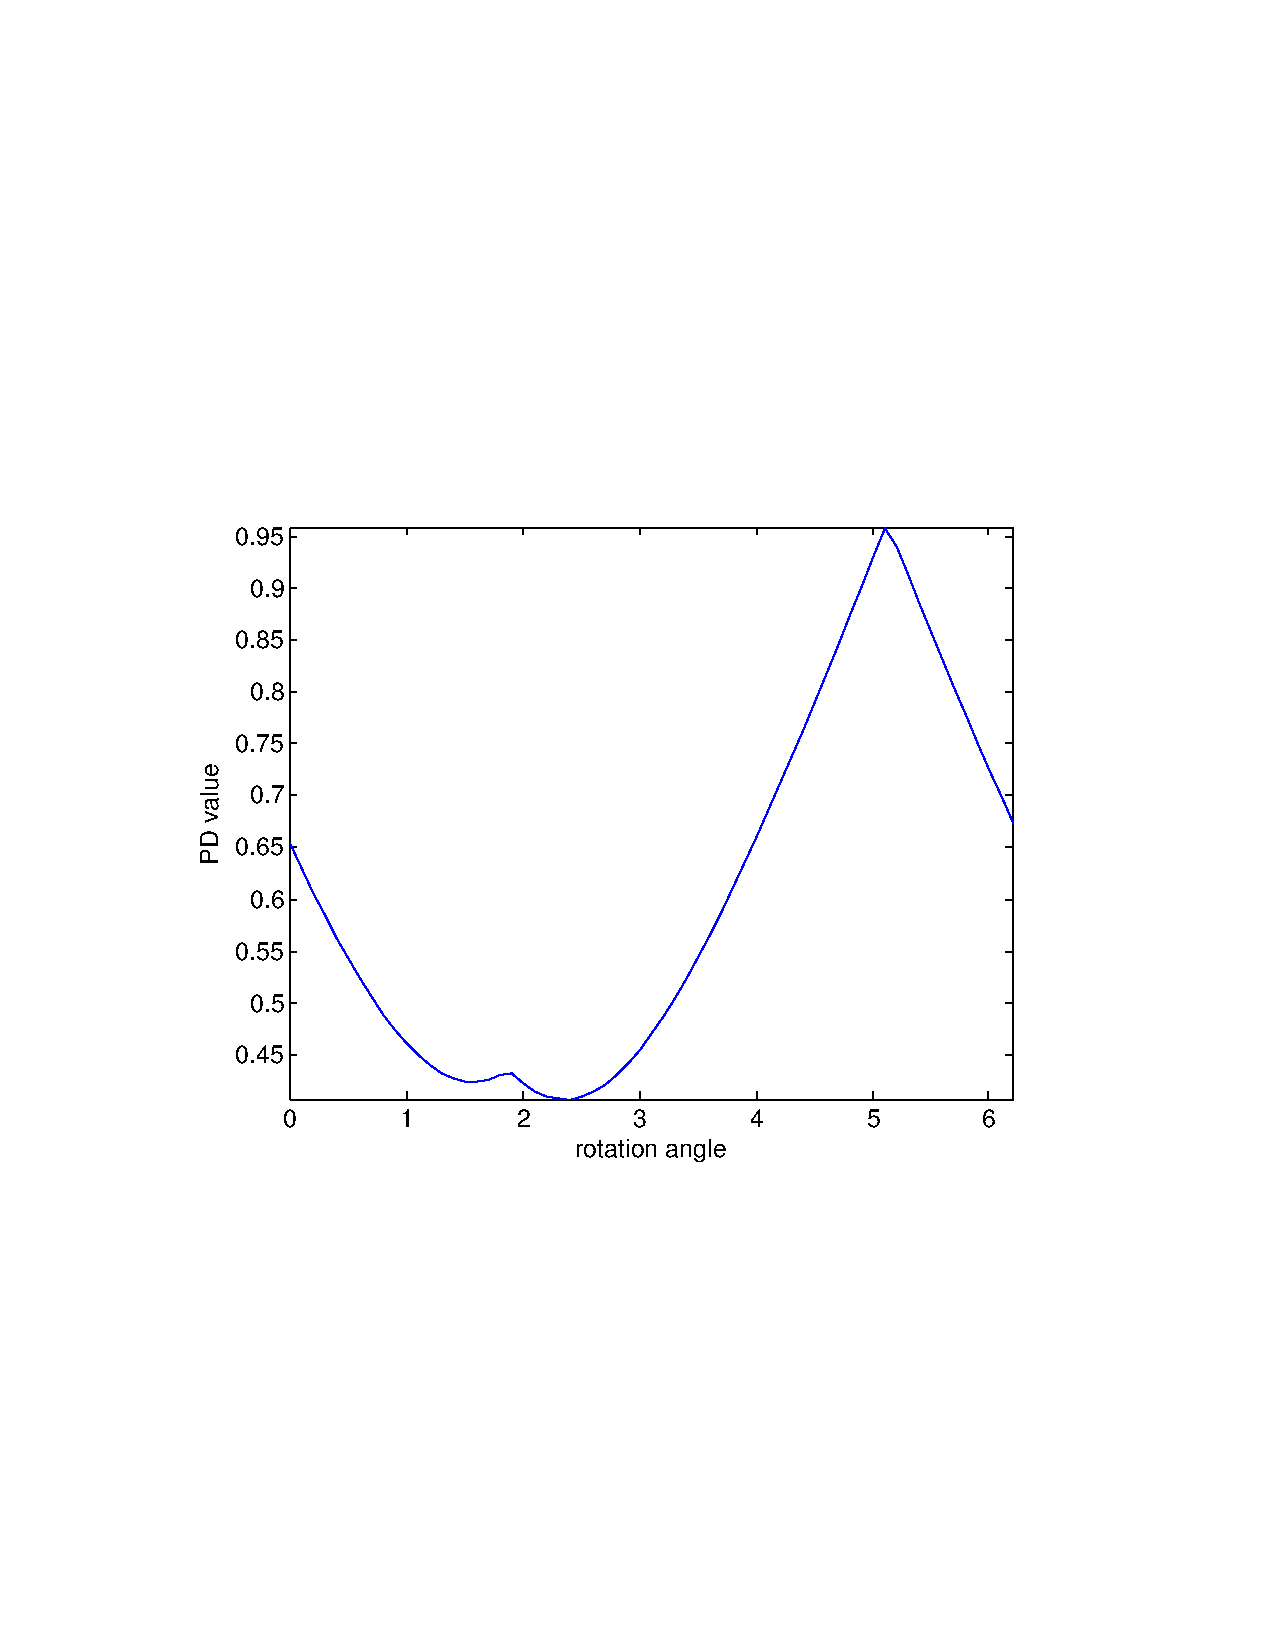
\includegraphics[width=0.33\linewidth, trim=33mm 80mm 40mm 85mm, clip]{figs/2/rotation_error_w01.pdf}}
  \subfloat[$\mu_i = 1$]{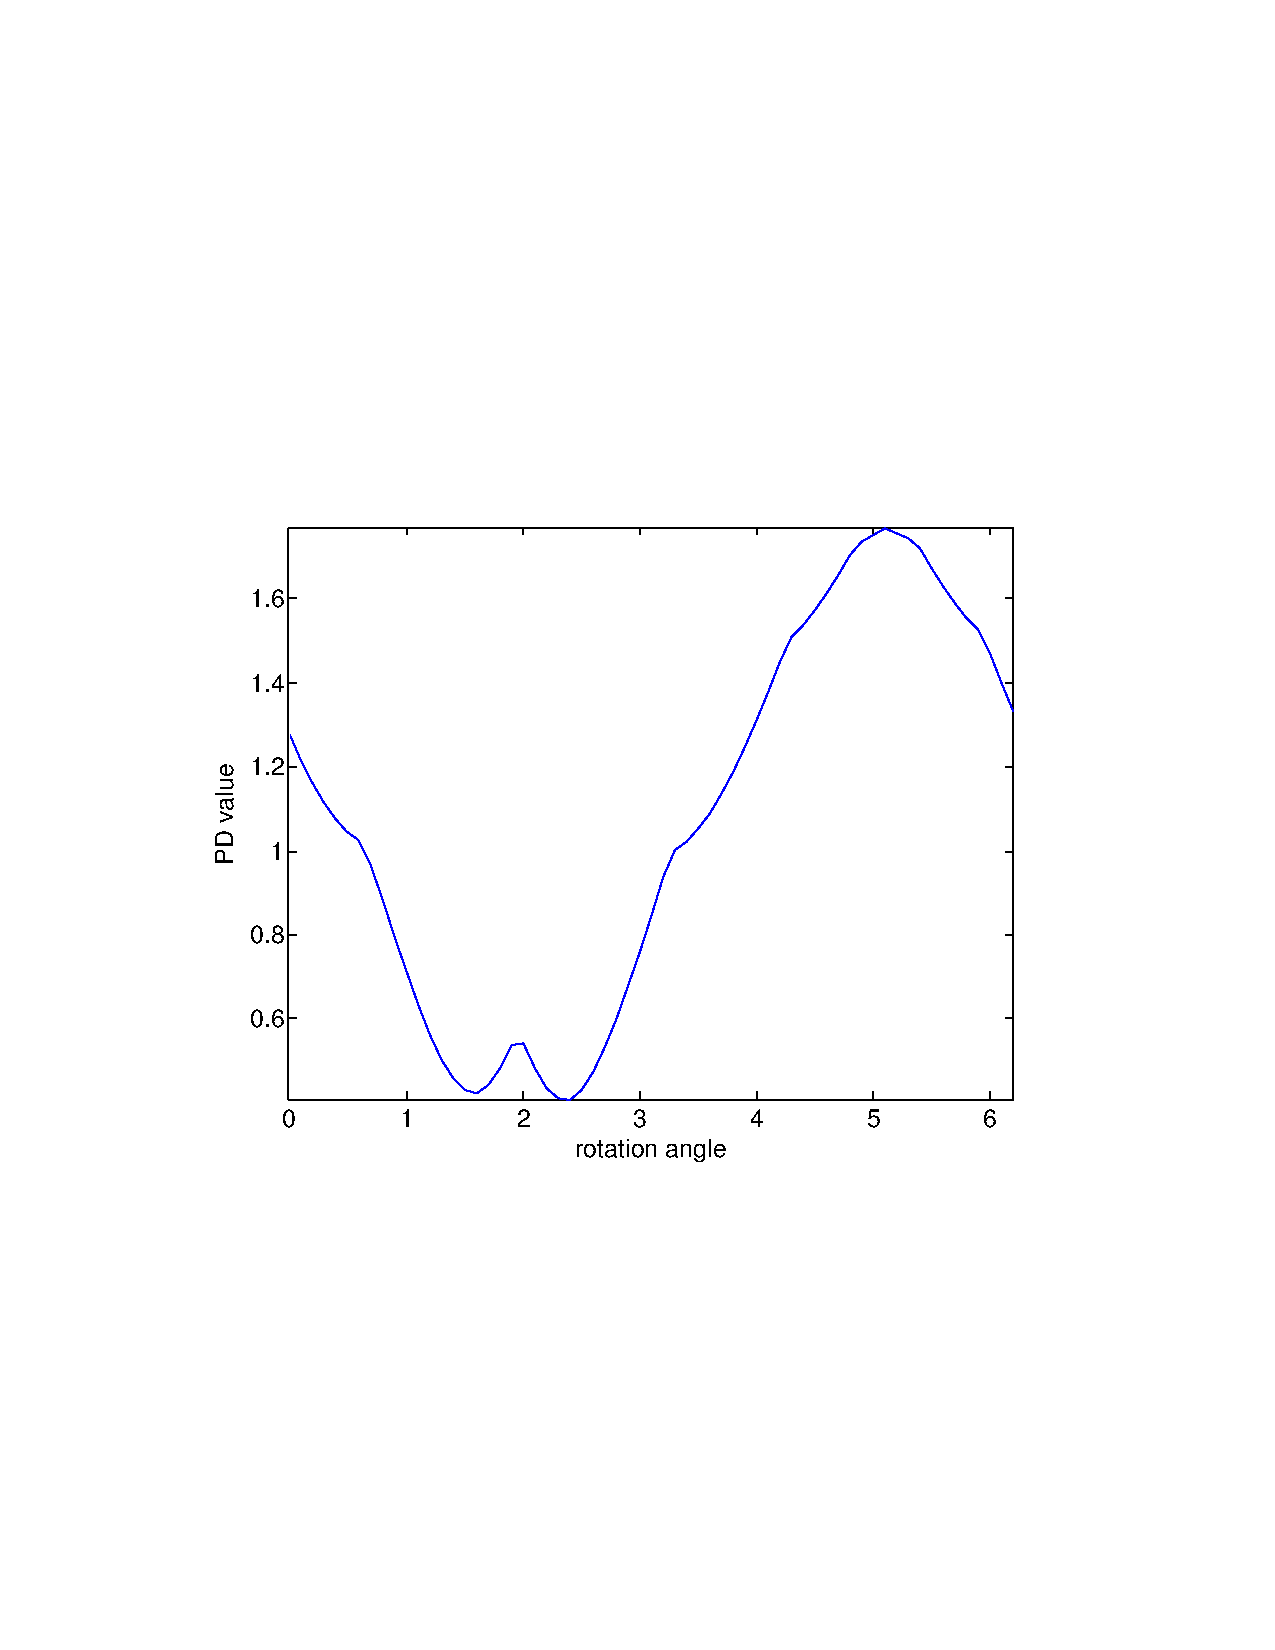
\includegraphics[width=0.33\linewidth, trim=33mm 80mm 40mm 85mm, clip]{figs/2/rotation_error_w1.pdf}}
  \subfloat[$\mu_i = 10$]{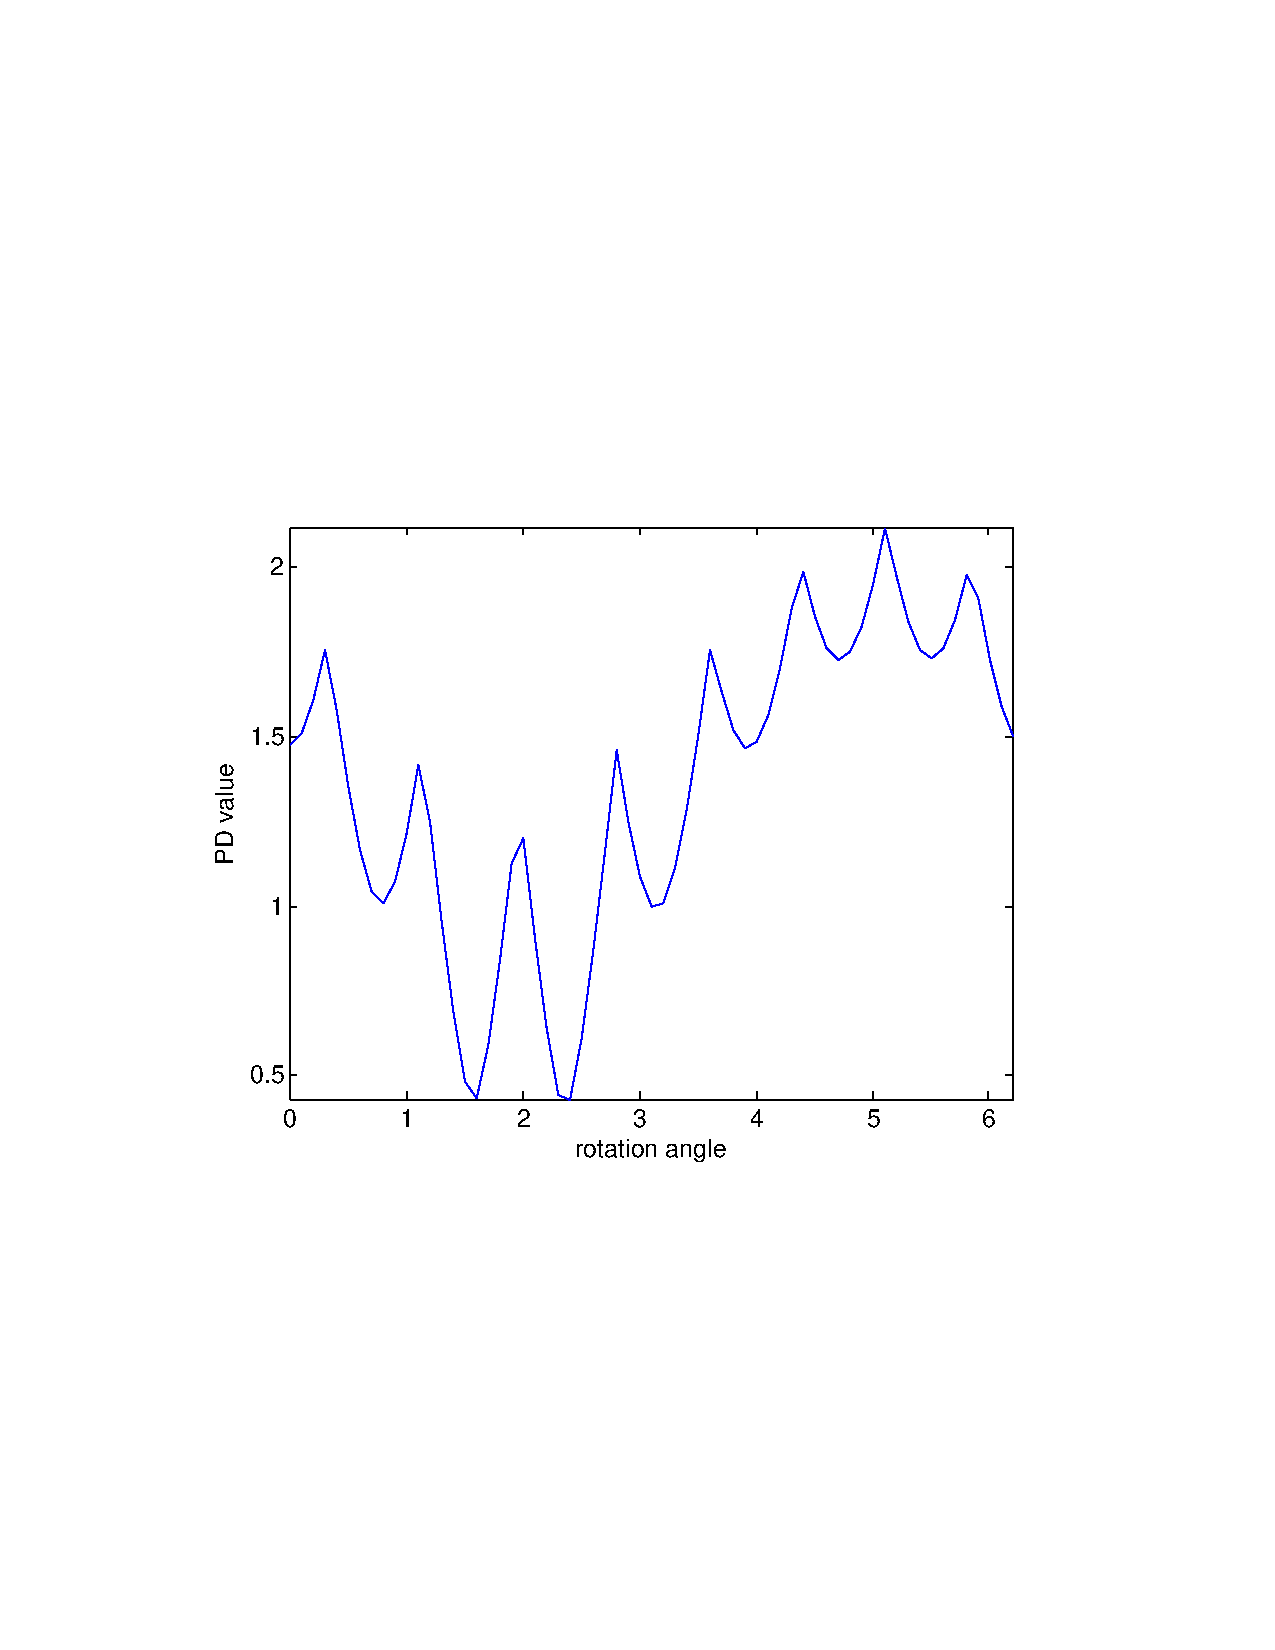
\includegraphics[width=0.33\linewidth, trim=33mm 80mm 40mm 85mm, clip]{figs/2/rotation_error_w10.pdf}} \\
  \subfloat[$\mu_i = 100$]{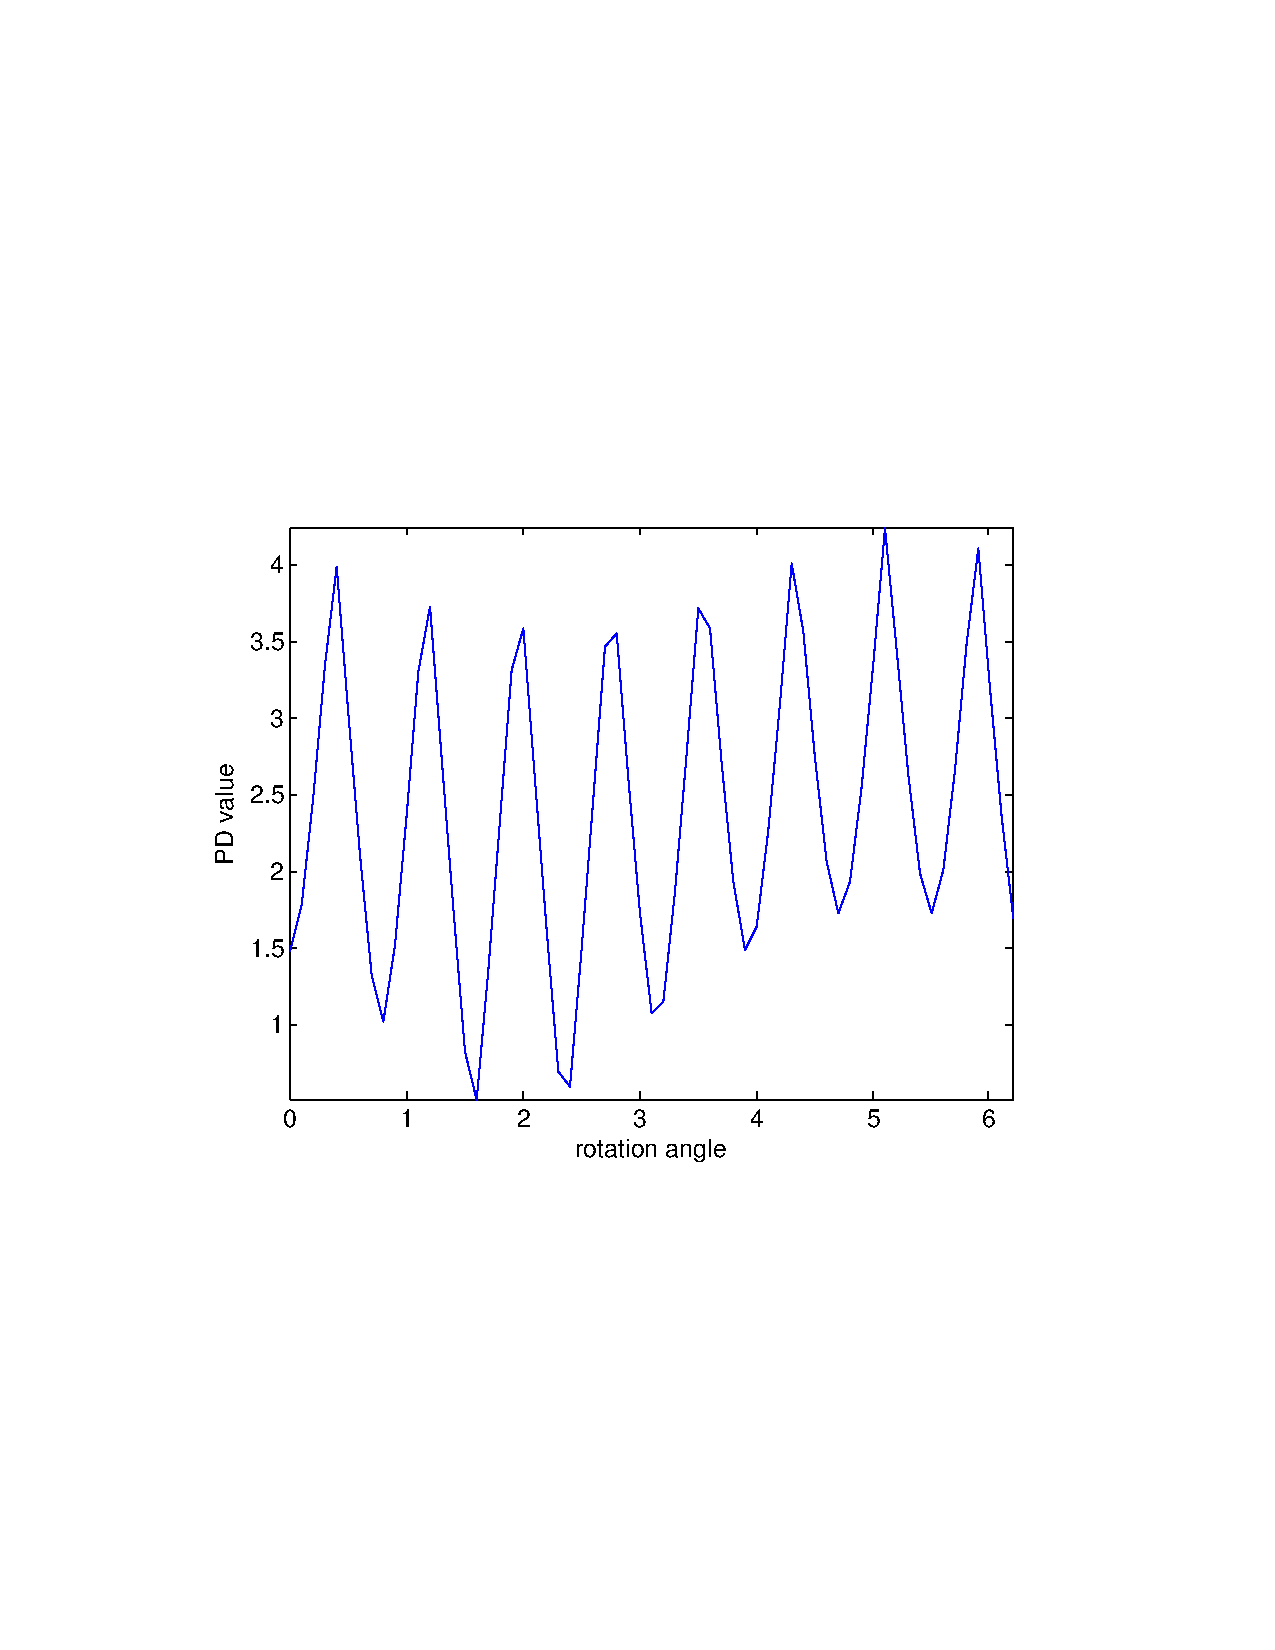
\includegraphics[width=0.33\linewidth, trim=33mm 80mm 40mm 85mm, clip]{figs/2/rotation_error_w100.pdf}}
  \subfloat[$\mu_i = 1,000$]{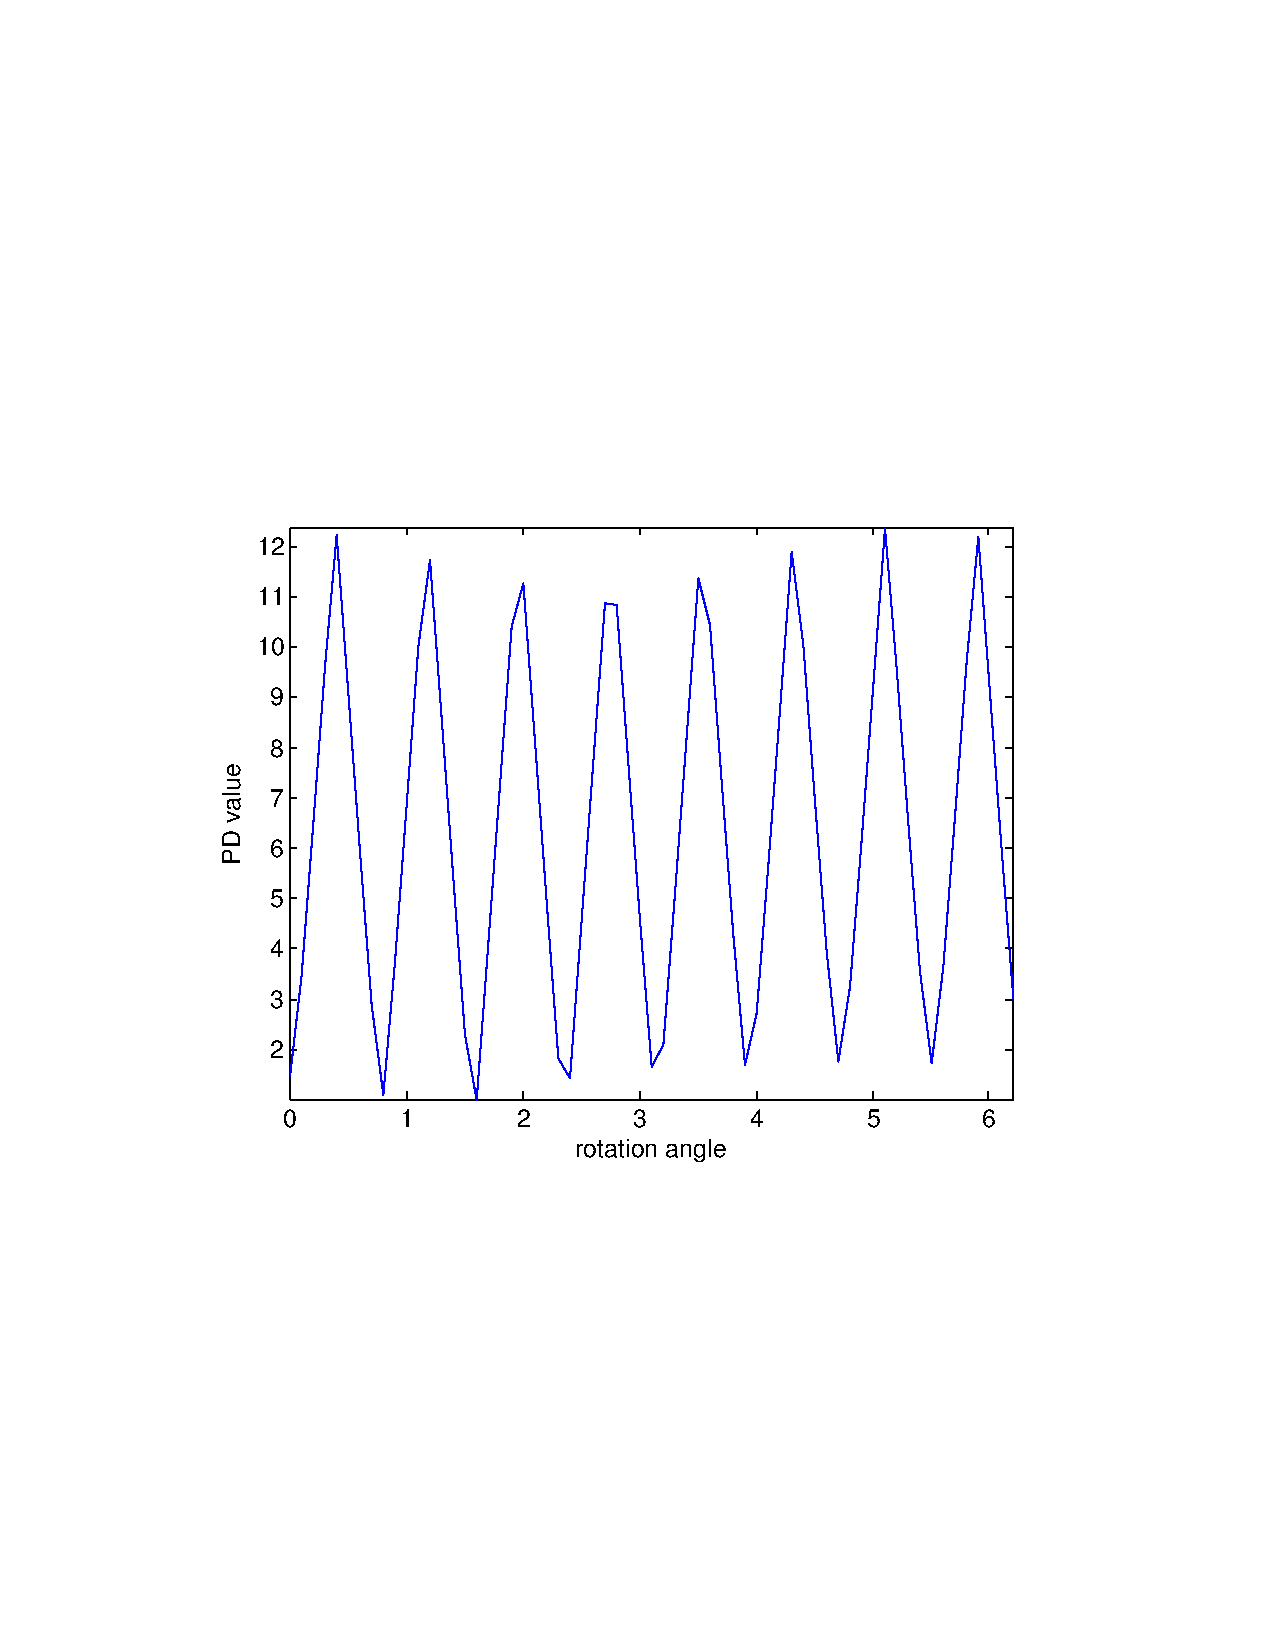
\includegraphics[width=0.33\linewidth, trim=33mm 80mm 40mm 85mm, clip]{figs/2/rotation_error_w1000.pdf}}
  \subfloat[$\mu_i = 10,000$]{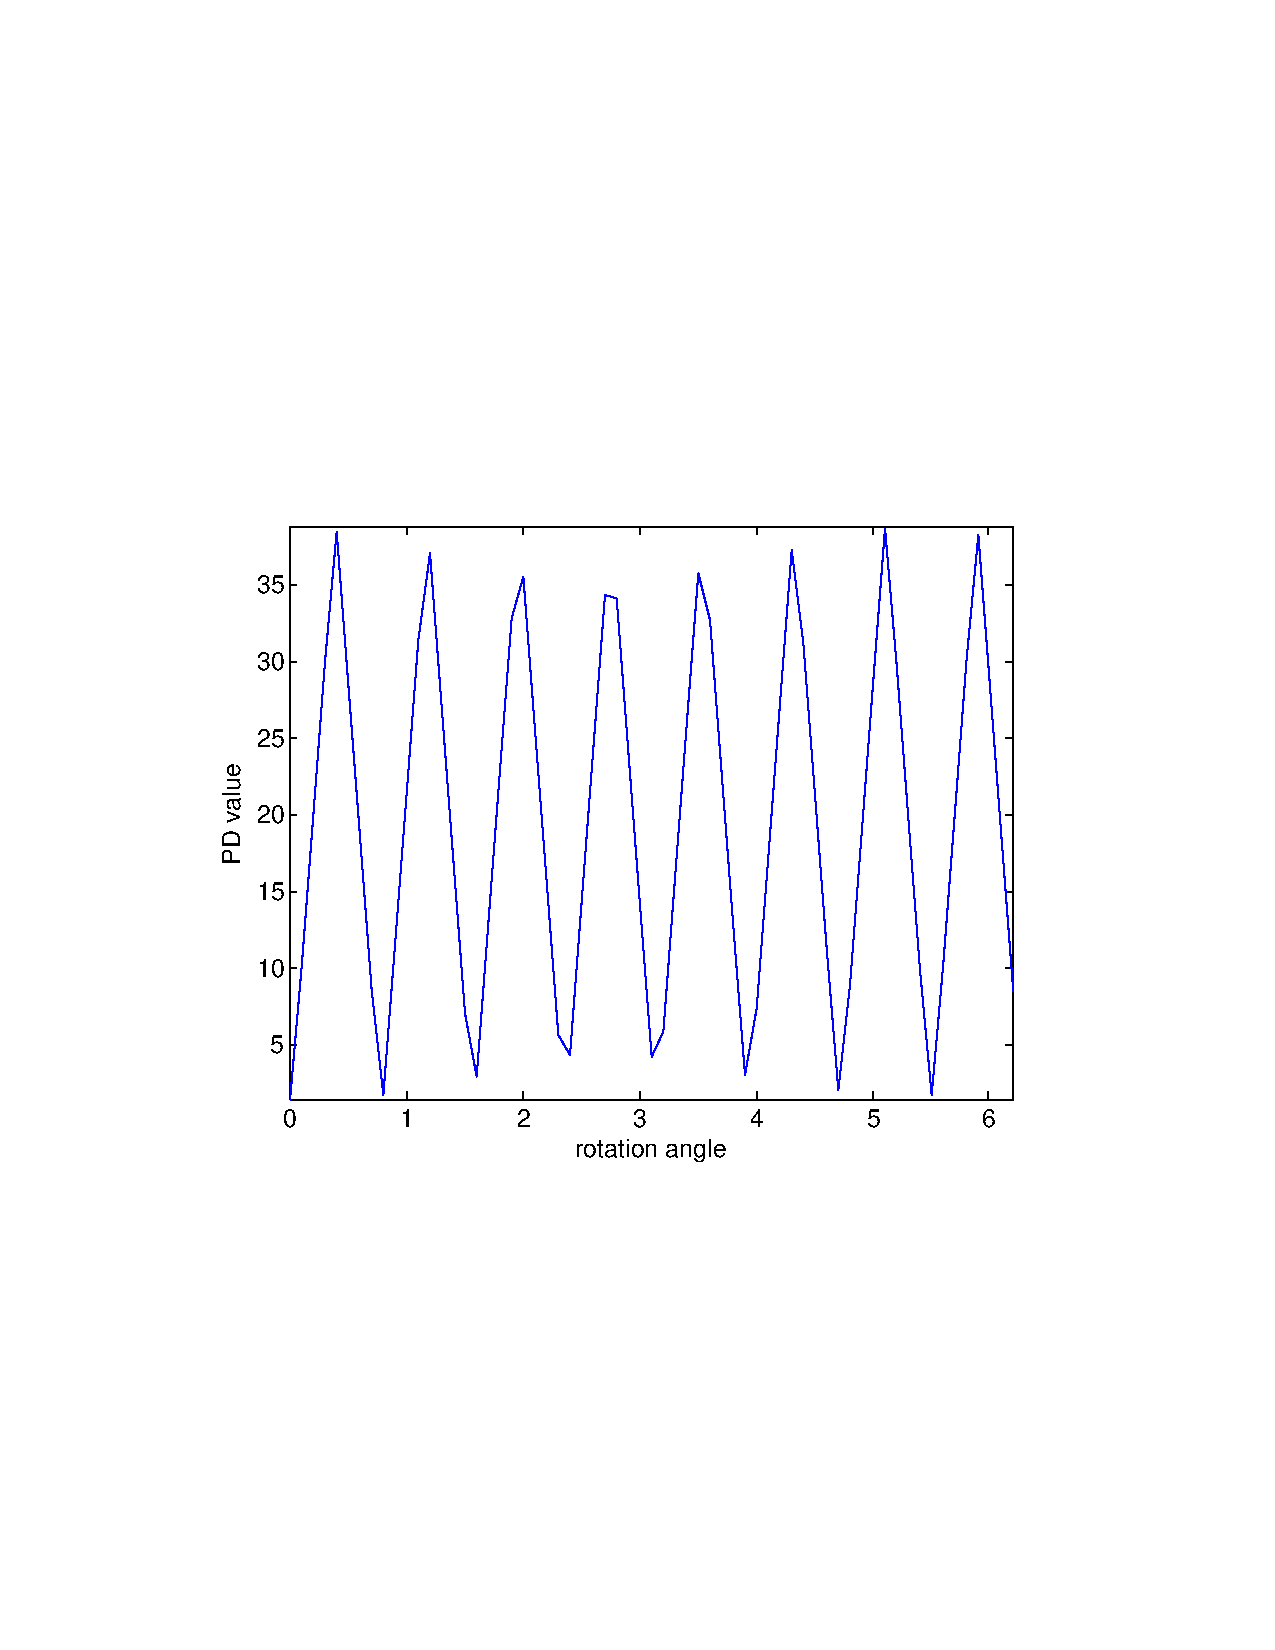
\includegraphics[width=0.33\linewidth, trim=33mm 80mm 40mm 85mm, clip]{figs/2/rotation_error_w10000.pdf}}
\caption[Configuration space metric's influence on the result of our PD algorithm: rotational example]{
The result of our PD algorithm on the rotational example shown in Figure~\ref{fig:2:toybenchmark}(a). We plot the PD values for all query configurations during the rotation, with different $\mu_i$ settings for the configuration space metric.
}\label{fig:2:rotation_error}
\end{figure}


\begin{figure}[!h]
\centering
  \subfloat[$\mu_i = 0$]{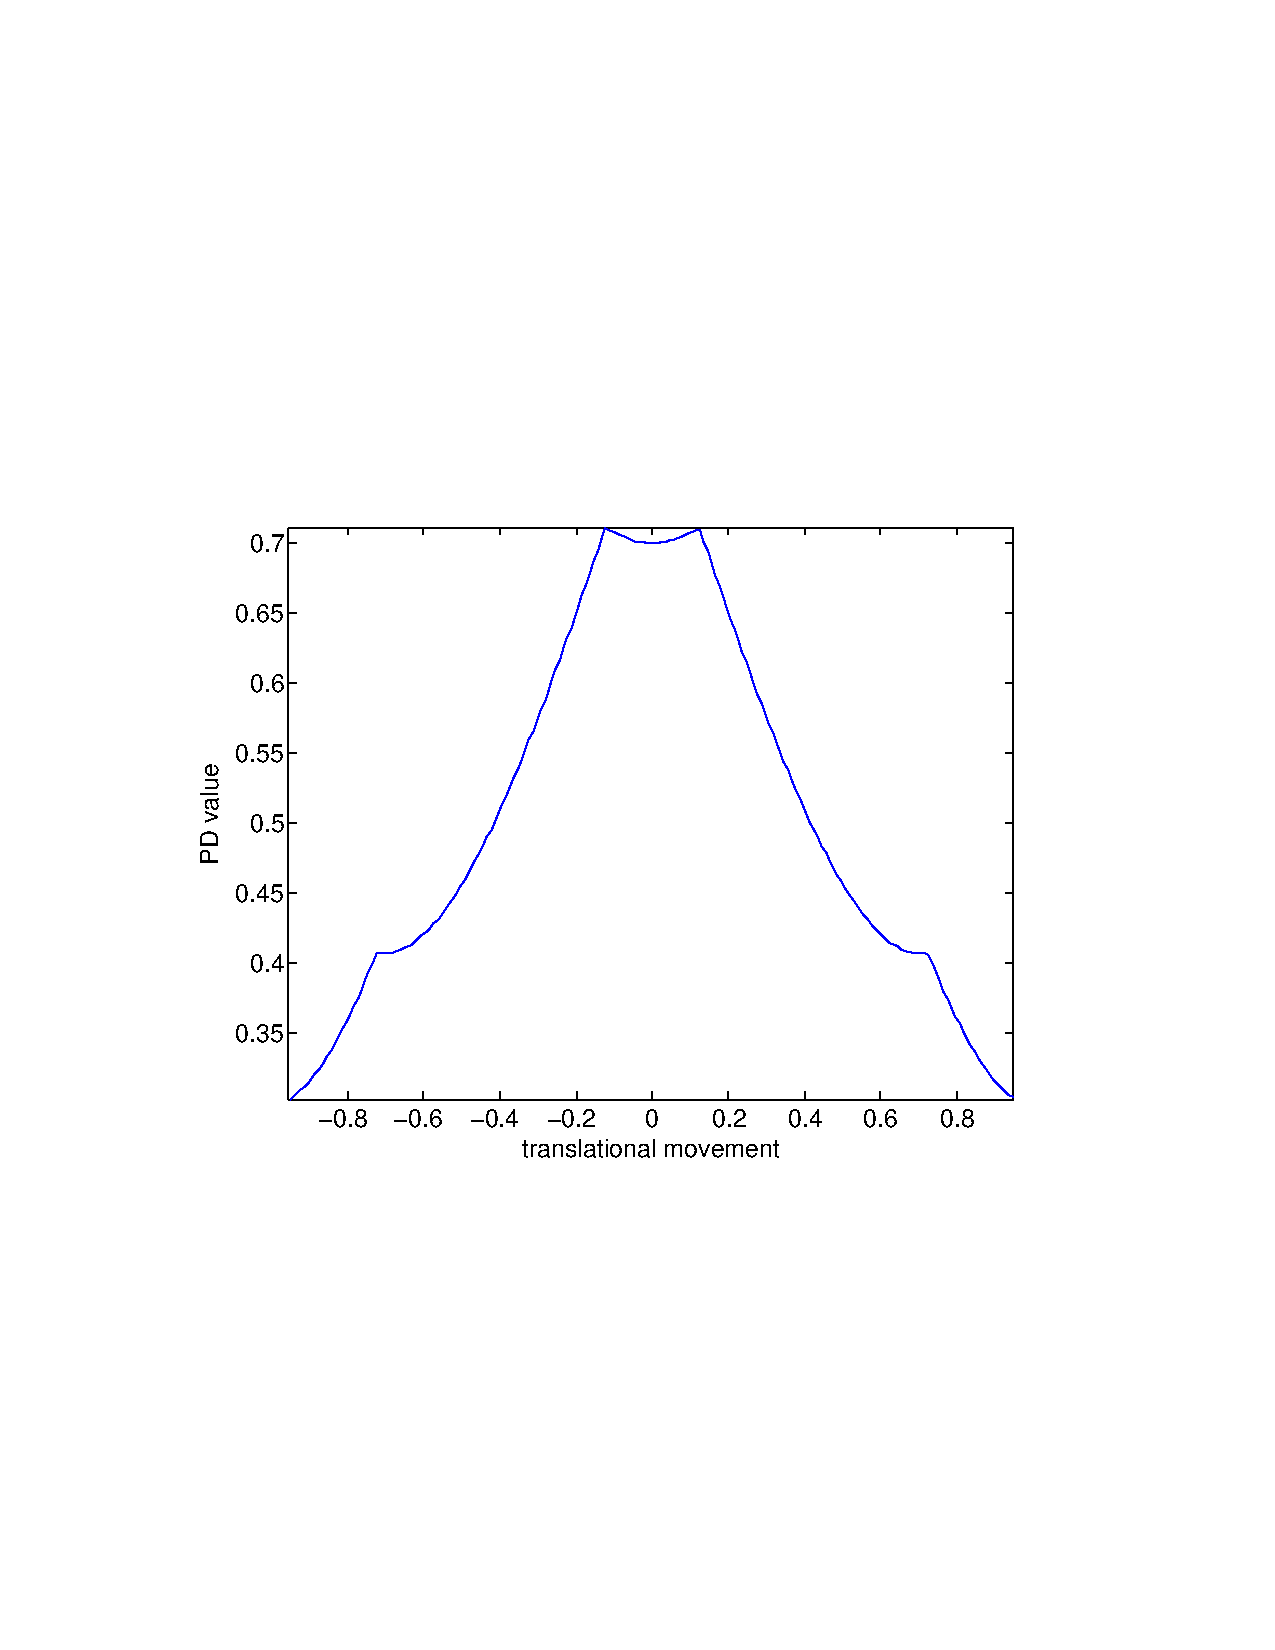
\includegraphics[width=0.33\linewidth, trim=33mm 80mm 40mm 85mm, clip]{figs/2/translation_error_w00000.pdf}}
  \subfloat[$\mu_i = 0.001$]{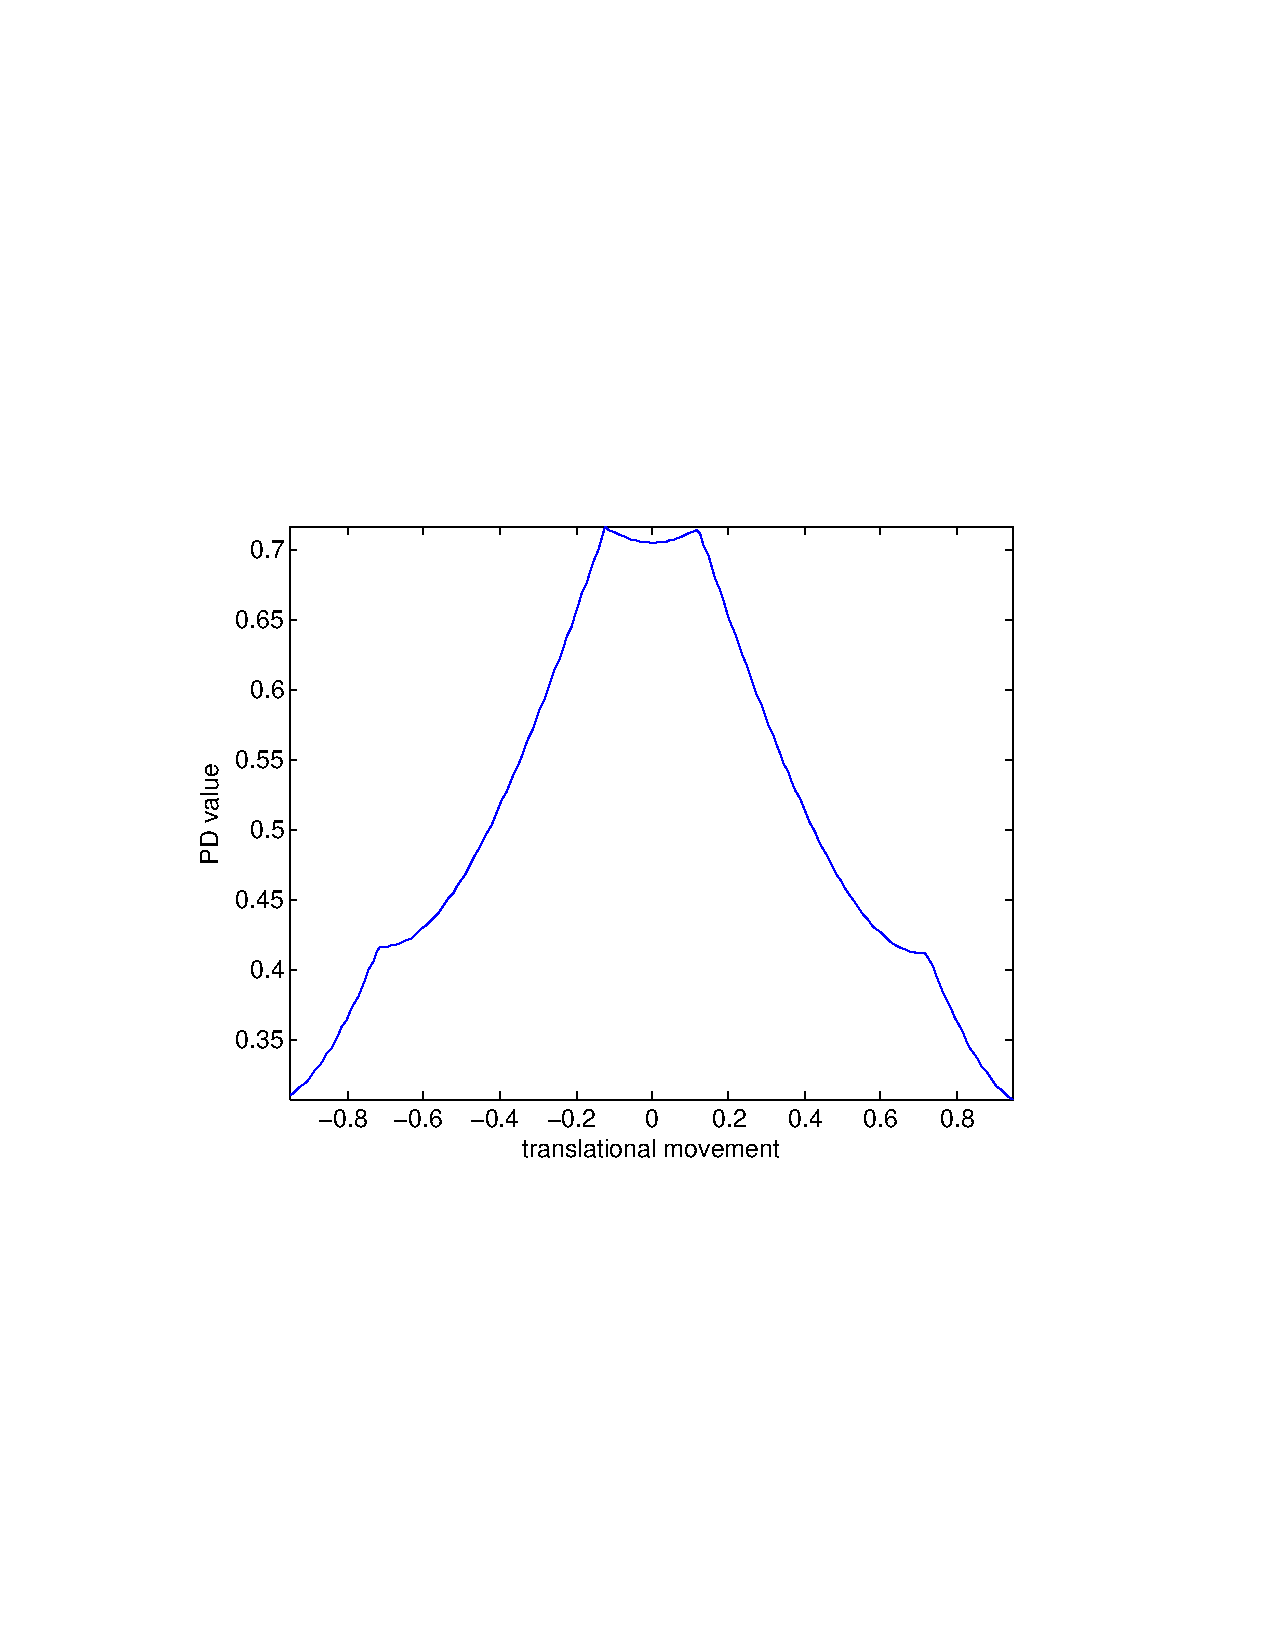
\includegraphics[width=0.33\linewidth, trim=33mm 80mm 40mm 85mm, clip]{figs/2/translation_error_w0001.pdf}} 
  \subfloat[$\mu_i = 0.01$]{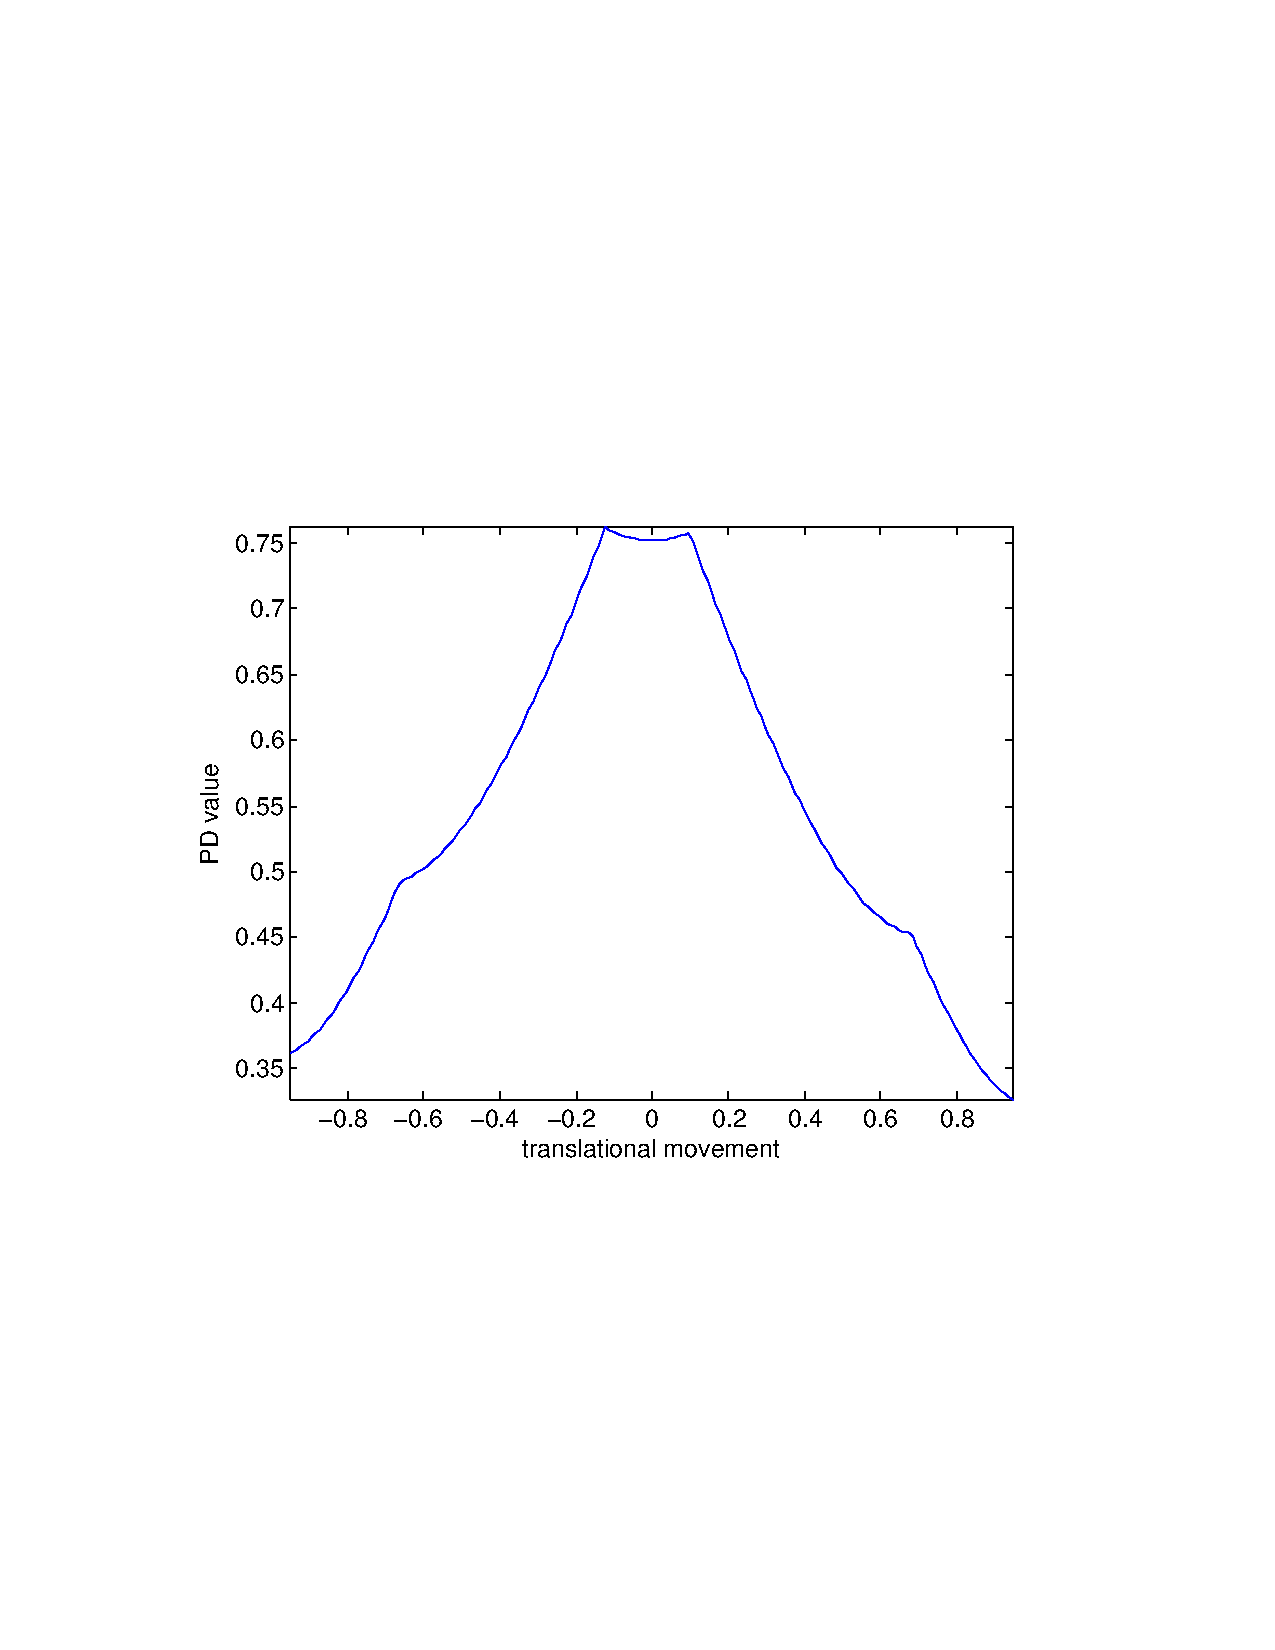
\includegraphics[width=0.33\linewidth, trim=33mm 80mm 40mm 85mm, clip]{figs/2/translation_error_w001.pdf}} \\
  \subfloat[$\mu_i = 0.1$]{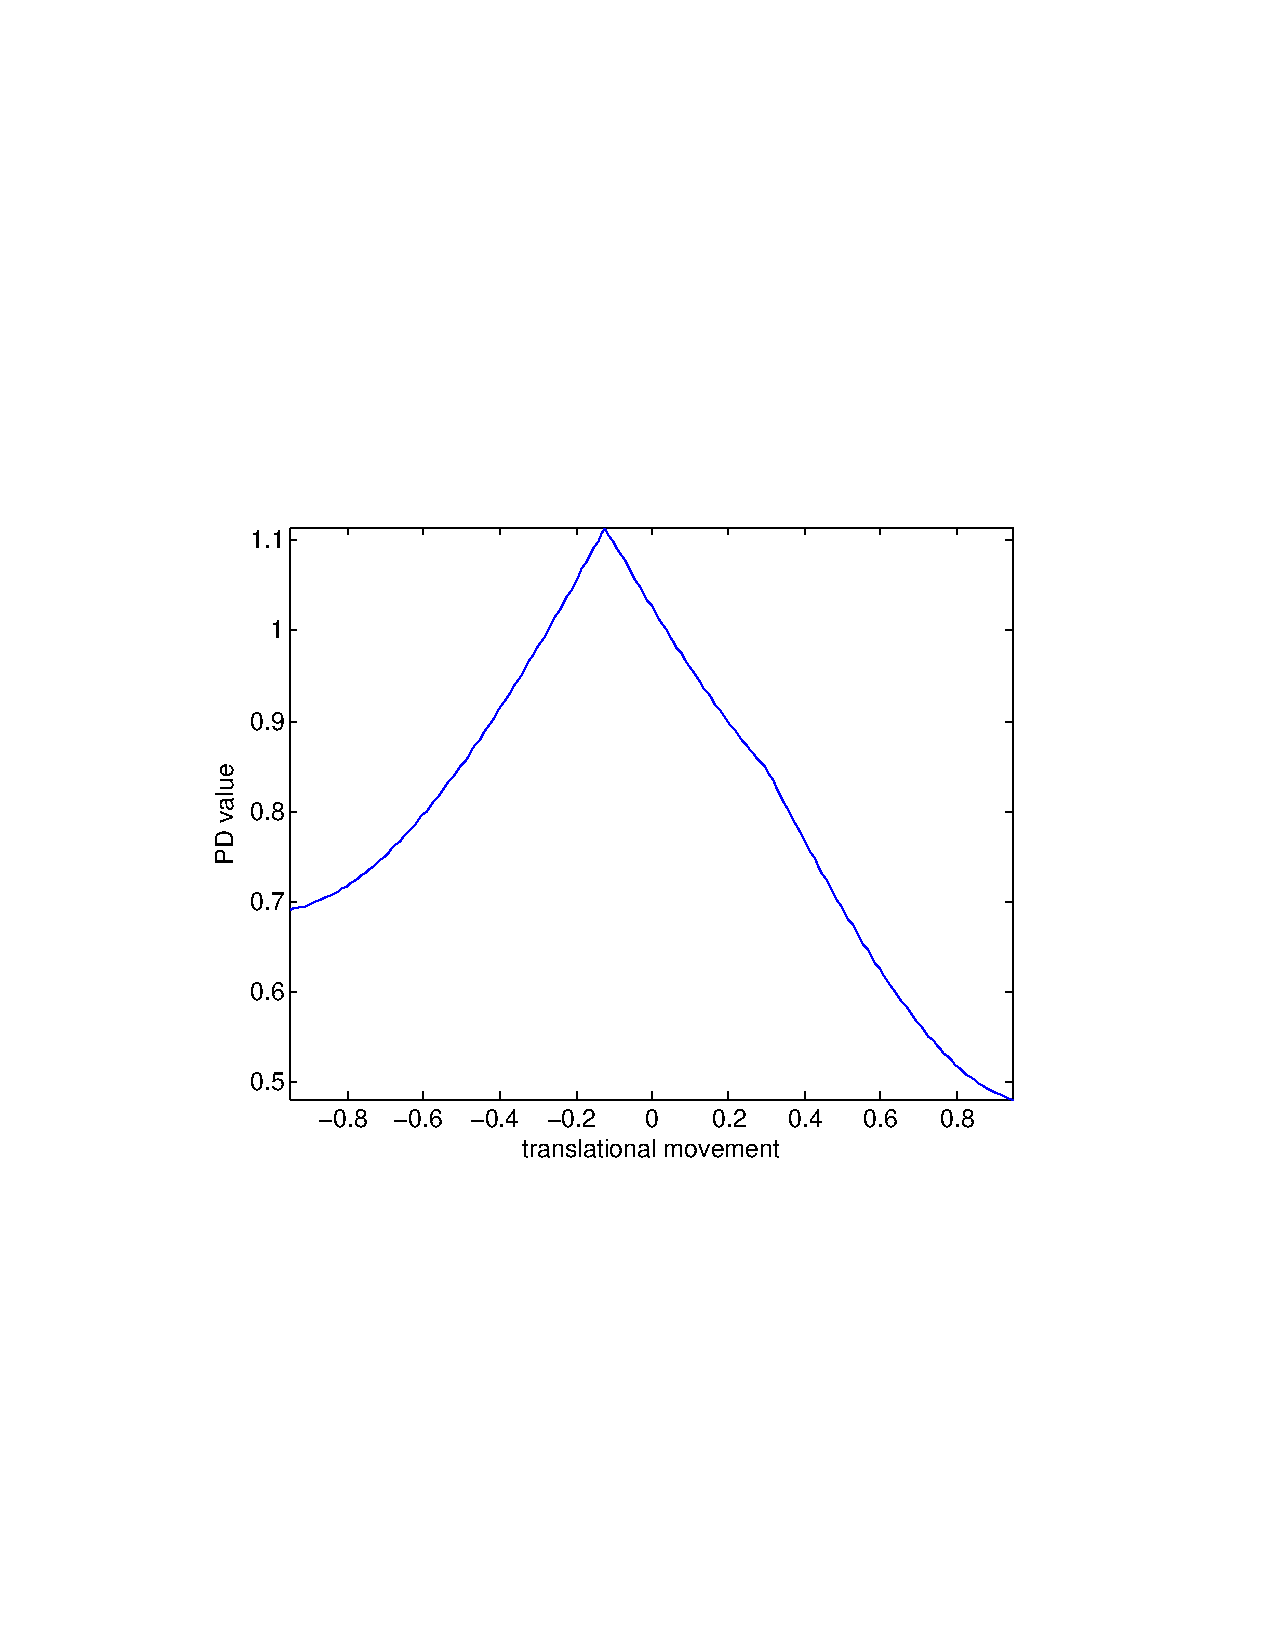
\includegraphics[width=0.33\linewidth, trim=33mm 80mm 40mm 85mm, clip]{figs/2/translation_error_w01.pdf}}
  \subfloat[$\mu_i = 1$]{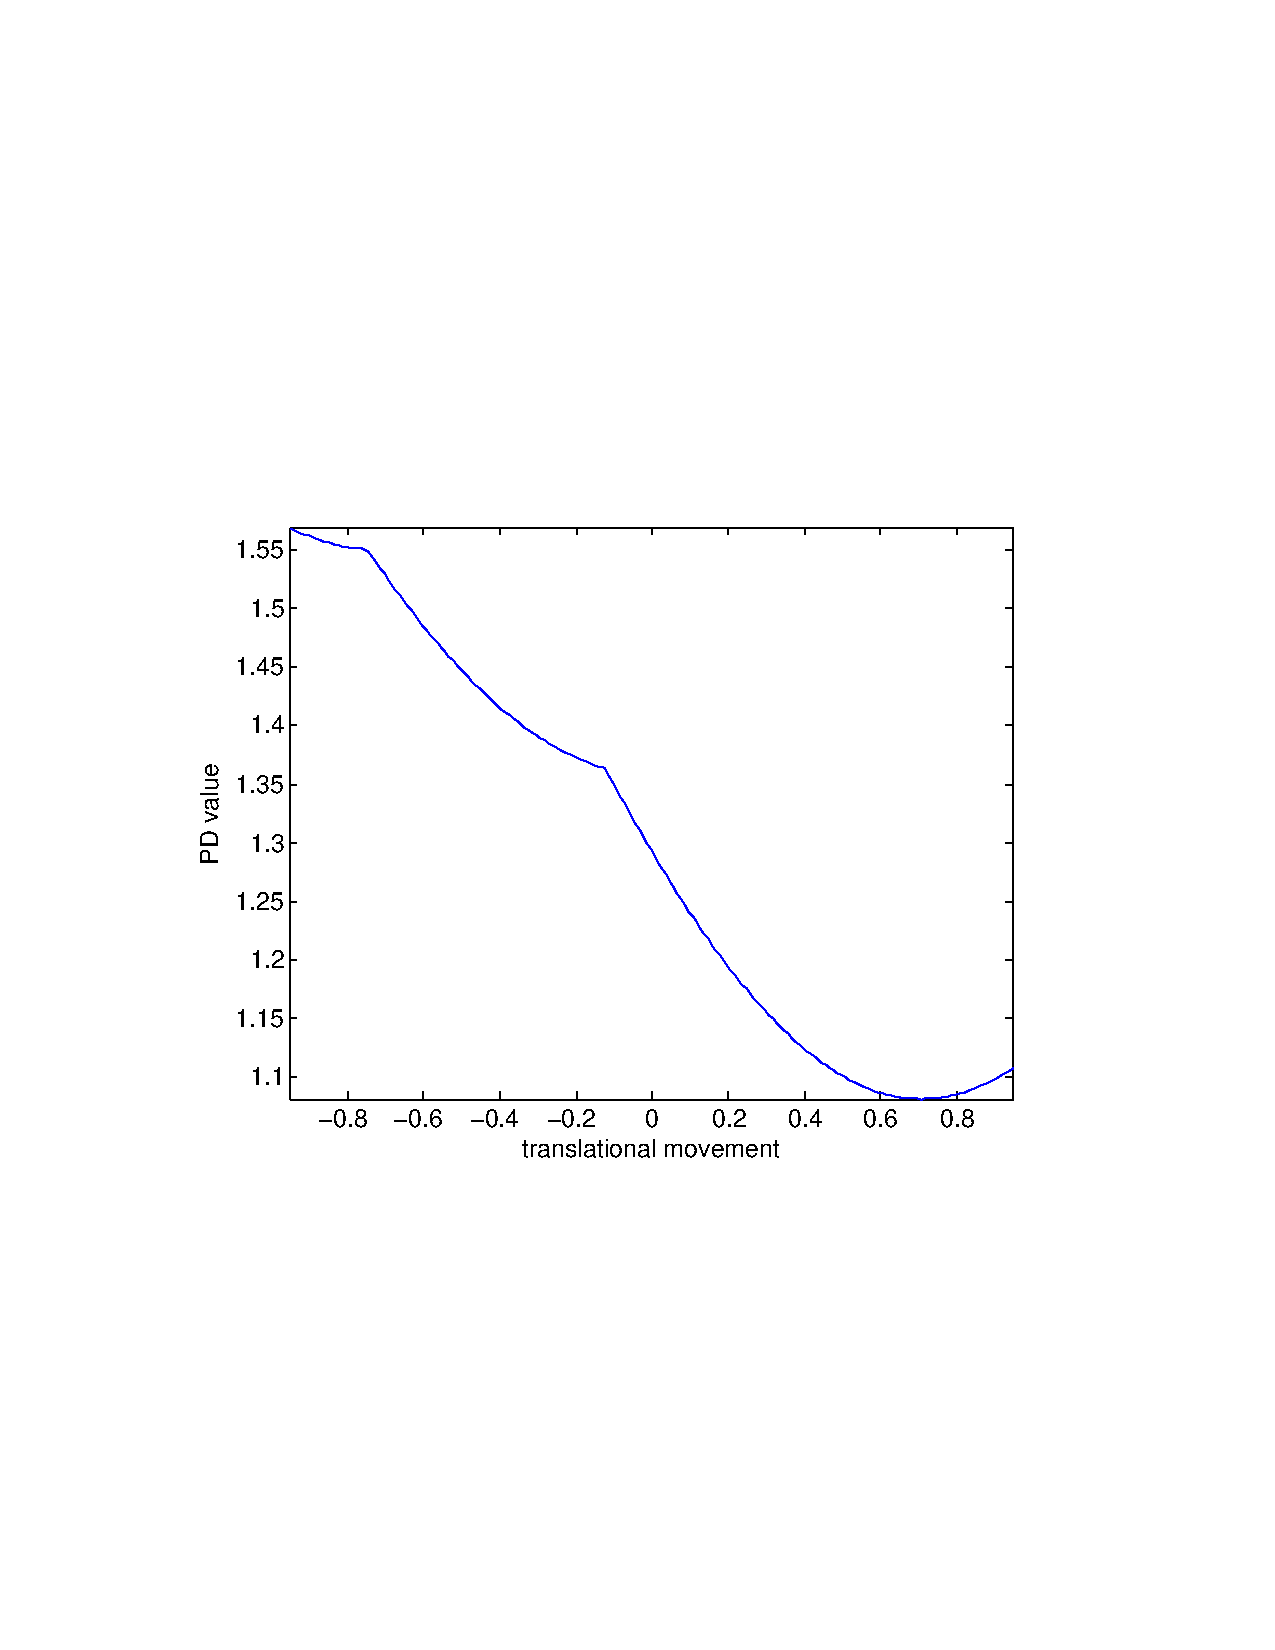
\includegraphics[width=0.33\linewidth, trim=33mm 80mm 40mm 85mm, clip]{figs/2/translation_error_w1.pdf}}
  \subfloat[$\mu_i = 10$]{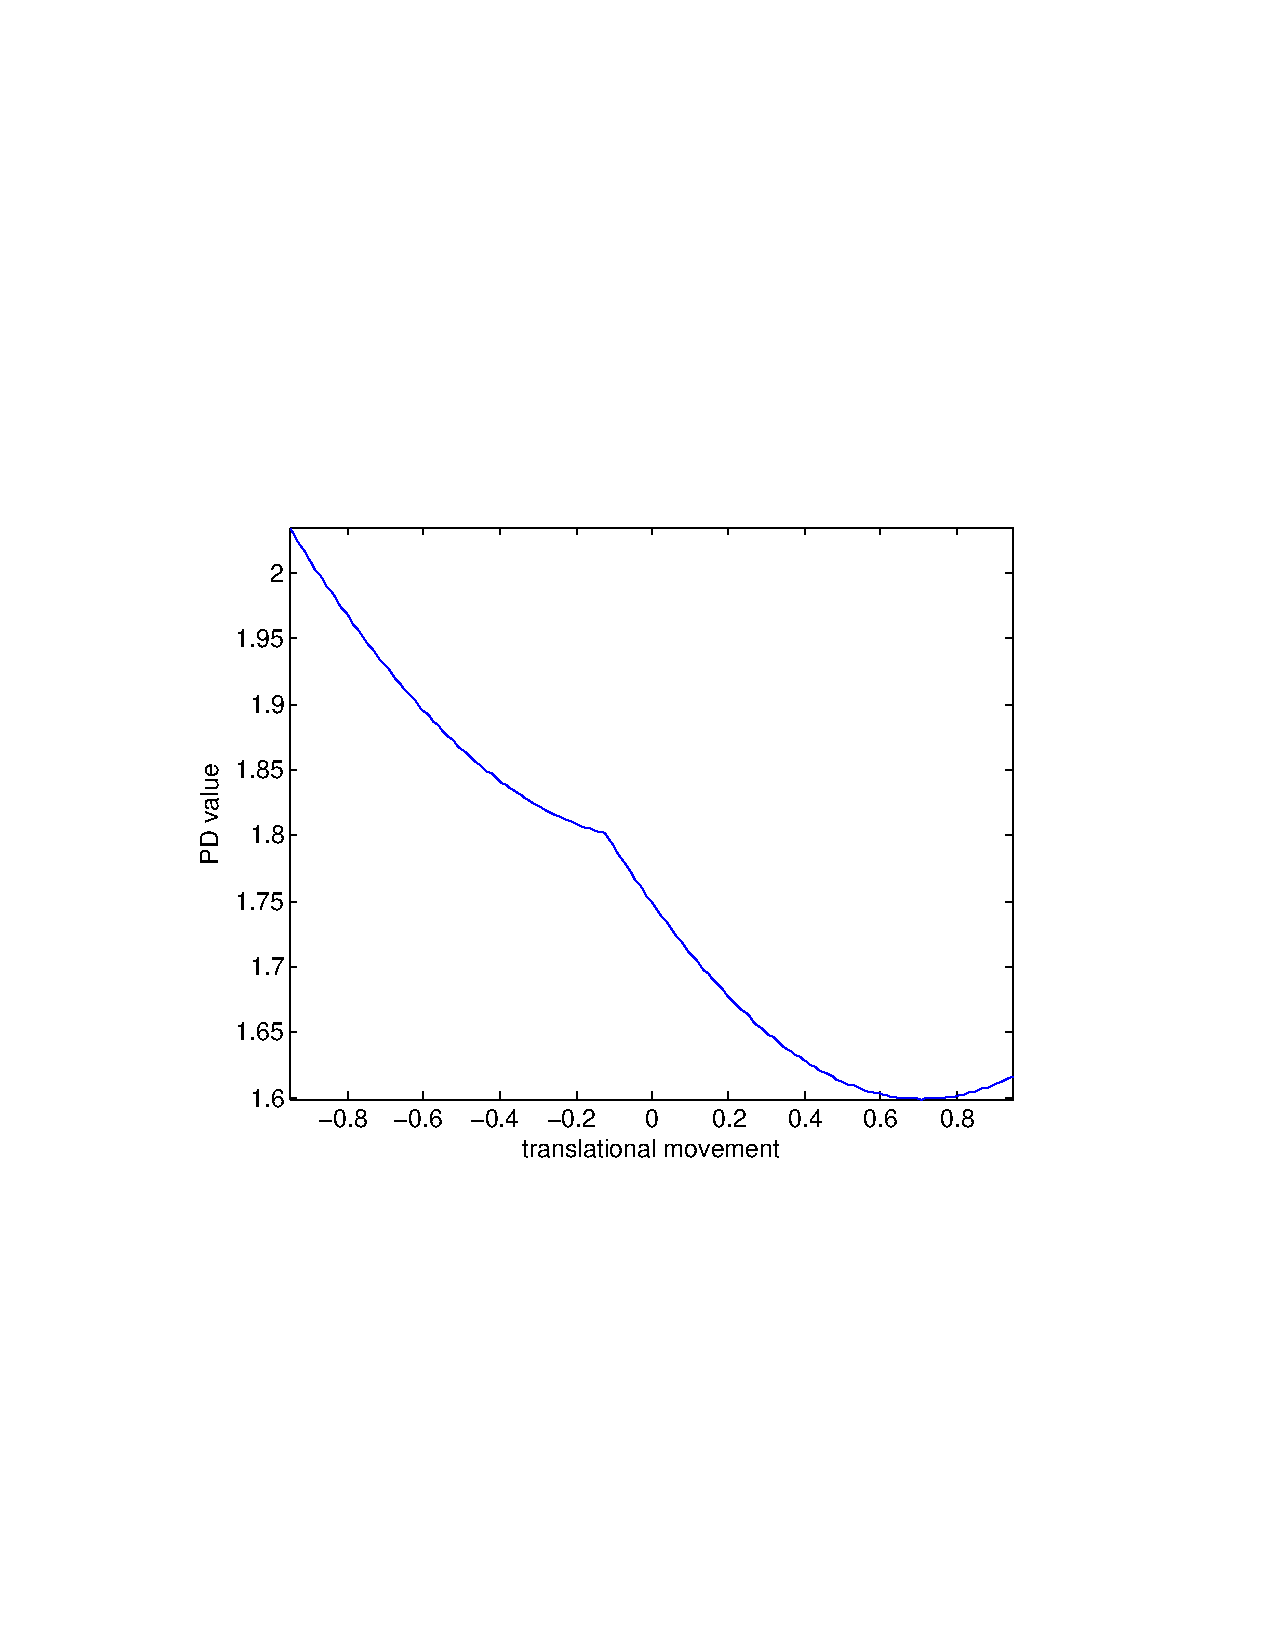
\includegraphics[width=0.33\linewidth, trim=33mm 80mm 40mm 85mm, clip]{figs/2/translation_error_w10.pdf}} \\
  \subfloat[$\mu_i = 100$]{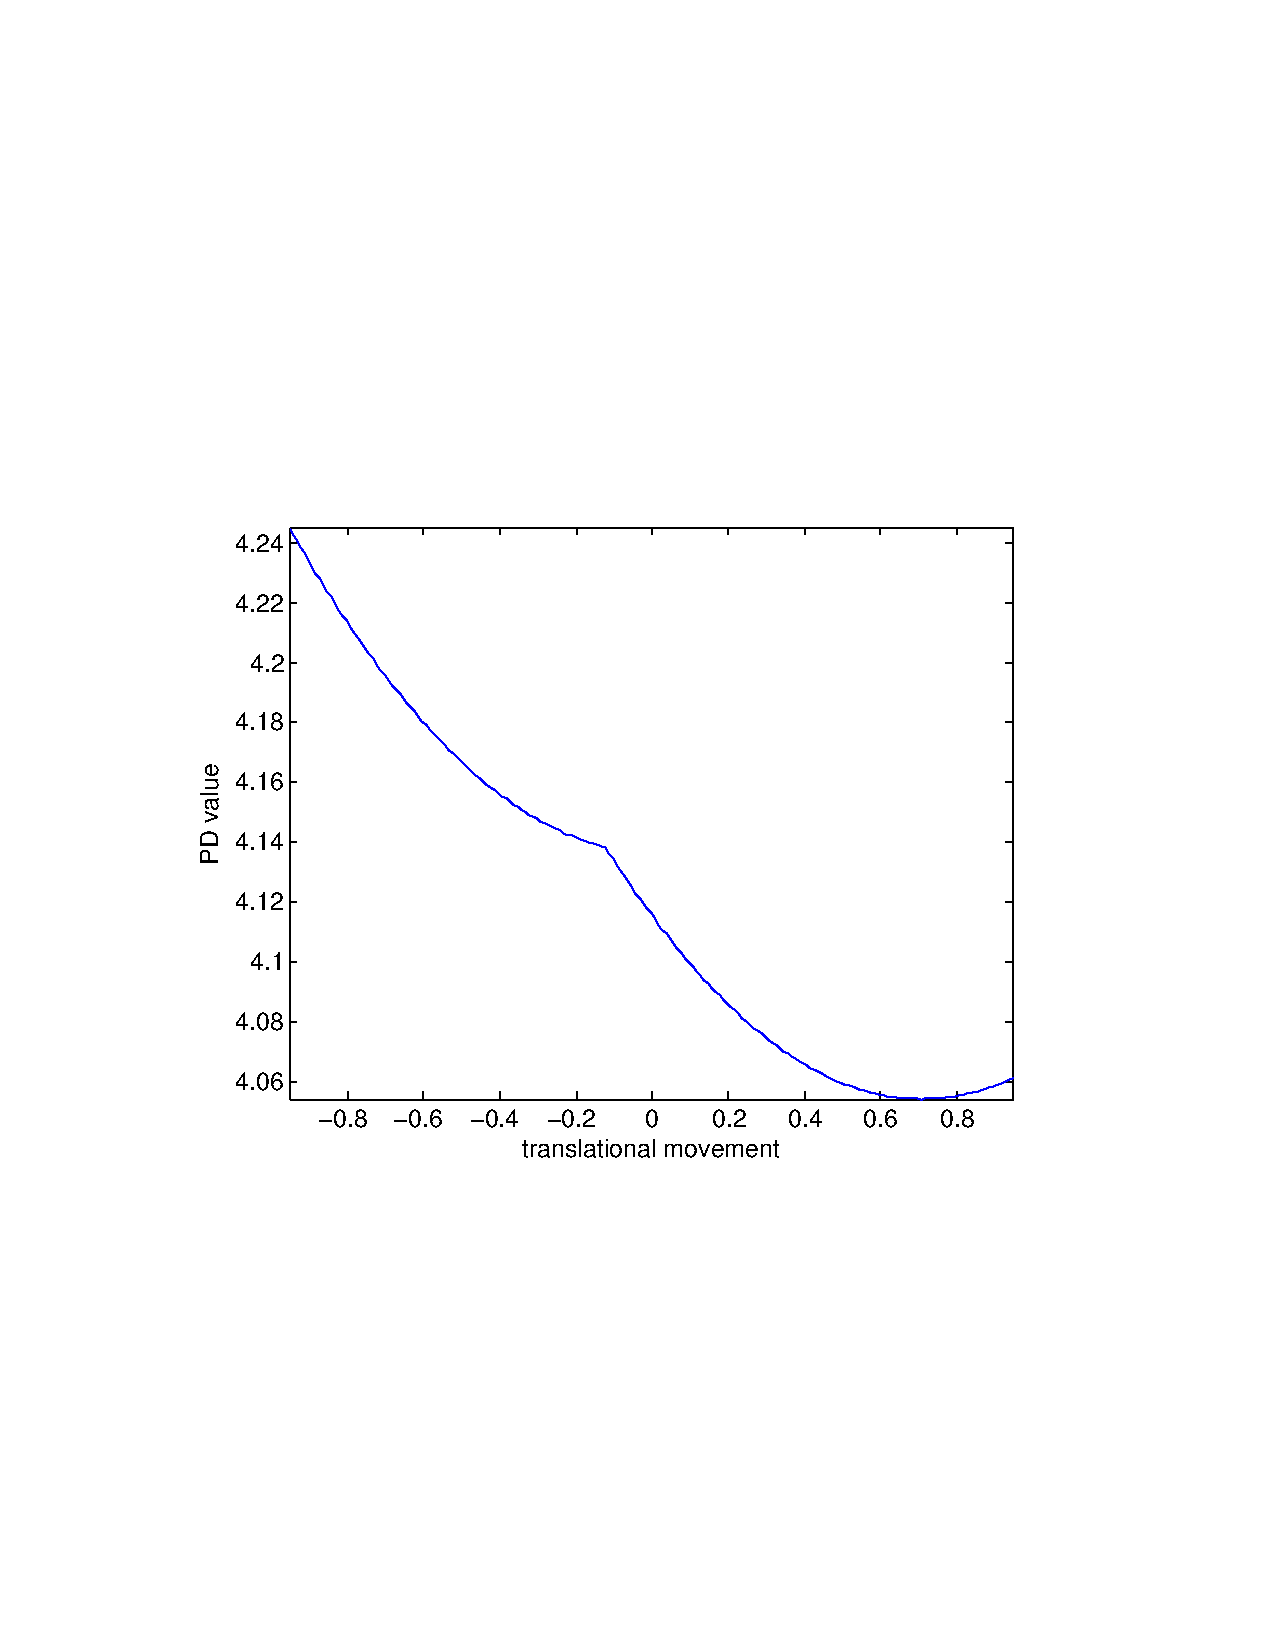
\includegraphics[width=0.33\linewidth, trim=33mm 80mm 40mm 85mm, clip]{figs/2/translation_error_w100.pdf}}
  \subfloat[$\mu_i = 1,000$]{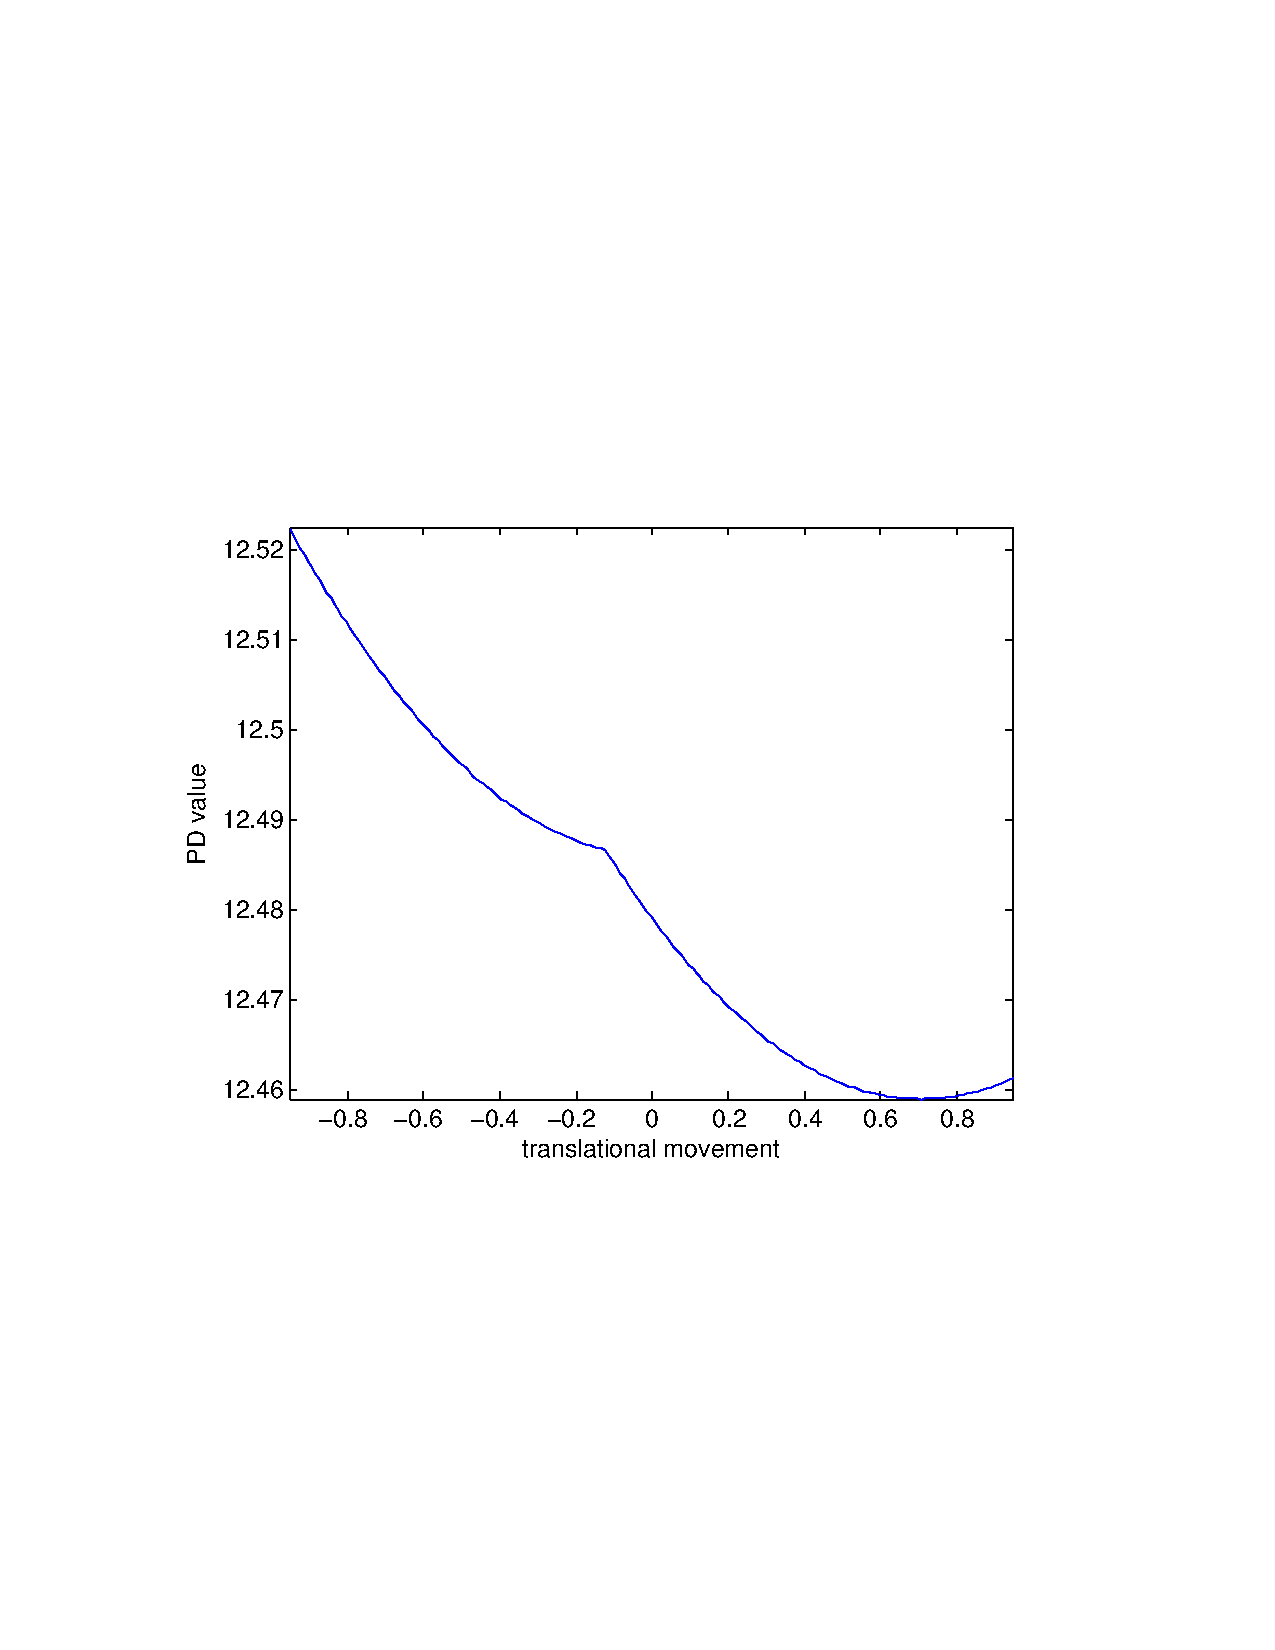
\includegraphics[width=0.33\linewidth, trim=30mm 80mm 40mm 85mm, clip]{figs/2/translation_error_w1000.pdf}}
  \subfloat[$\mu_i = 10,000$]{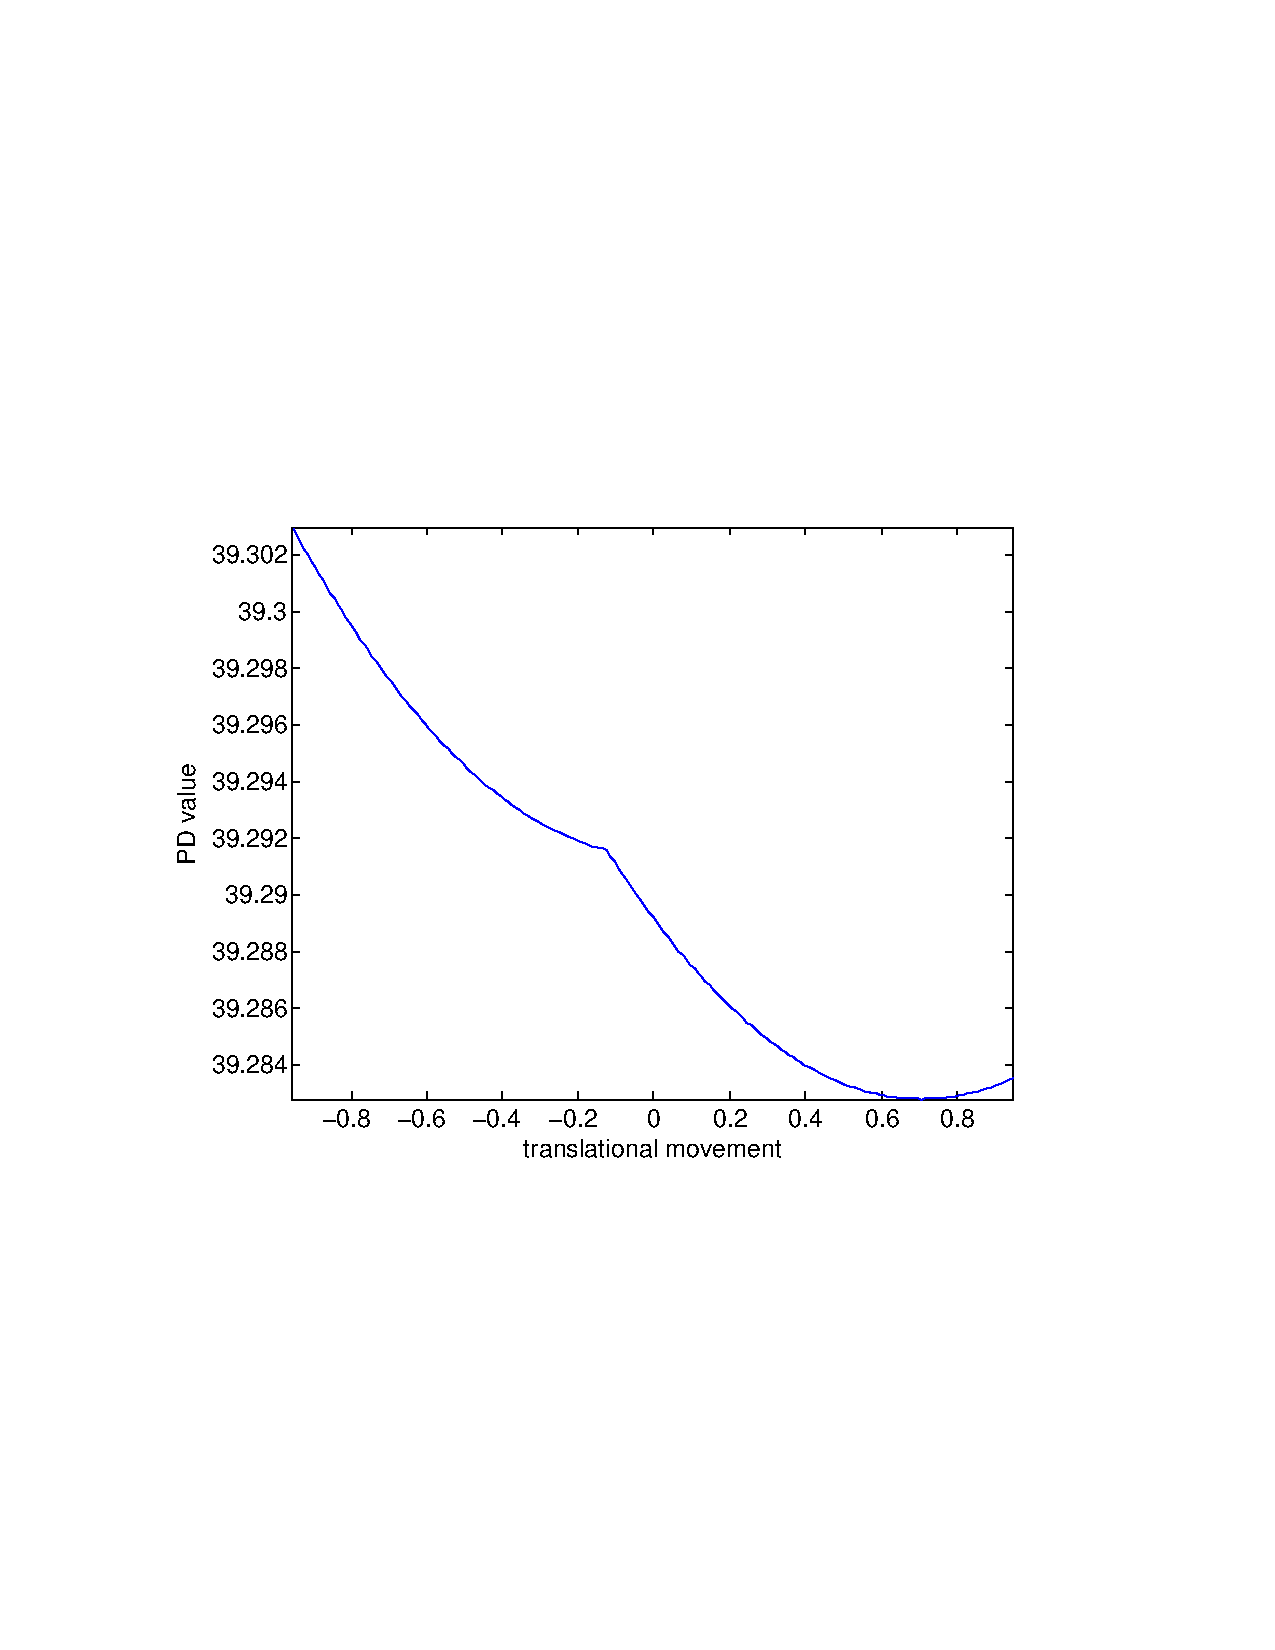
\includegraphics[width=0.33\linewidth, trim=30mm 80mm 40mm 85mm, clip]{figs/2/translation_error_w10000.pdf}}
\caption[Configuration space metric's influence on the result of our PD algorithm: translational example]{The result of our PD algorithm on the translational example shown in Figure~\ref{fig:2:toybenchmark}(b). We plot the PD values for all query configurations during the translation, with different $\mu_i$ settings for the configuration space metric.}\label{fig:2:translation_error}
\end{figure}

In the first example (Figure~\ref{fig:2:toybenchmark}(a)), the moving object only performs counter-clockwise rotation. The query's rotation angle is $0$ at the beginning and then incrementally increases to $2\pi$ in steps of $\pi/4$. If large weights are assigned to the configuration space metric (i.e., $\mu_i$ values are large in Equation~\ref{eq:PDgmetricMu}), the query's closest neighbor among the eight contact-space samples would be $\mathbf q_1$, corresponding to a rotation angle of $0$. When the query's rotation angle increases from $0$ to $\pi/4$, the corresponding PD value will first increase and then decrease. This is because the PD value is dominated by the difference in rotation angles: when the rotation angle is close to $0$ or $\pi/4$, this query is either close to $\mathbf q_1$ or to $\mathbf q_2$ respectively, and thus the corresponding PD value is small; when the rotation angle is near $\pi/8$, this query is far from both $\mathbf q_1$ and $\mathbf q_2$, and thus the corresponding PD value is large. This phenomenon is shown in Figure~\ref{fig:2:rotation_error}(f)-(i). From these results for large $\mu_i$ values, we also observe significant vibrations in PD values when the rotation angle changes. The magnitude of such vibrations decreases when parameters $\mu_i$ become smaller (Figures~\ref{fig:2:rotation_error}(a)-(e)). In Figure~\ref{fig:2:rotation_error}(a), PD values are constant when $\mu_i = 0$, since rotational weights in the object norm metric are zero.

In the second example (Figure~\ref{fig:2:toybenchmark}(b)), the moving object only performs translational motion. At the beginning, the object is in contact with the obstacles. It then moves deep inside the obstacles along the $y$-axis till it finally comes into contact with the obstacle again and then separates from the obstacle. During this motion, the moving object's rotation angle is fixed at $\pi/8$. The results of our PD algorithm are shown in Figure~\ref{fig:2:translation_error}. For all $\mu_i$ values, PD values are non-zero for in-contact configurations at the beginning and end of the movement. As we discussed above, this is because we only use a finite number of in-contact configurations to approximate the contact space, and none of them have the same rotation angle ($\pi/8$) as the query. However, if $\mu_i$ is small (Figures~\ref{fig:2:translation_error}(a)-(d)), PD values first increase and then decrease, which is consistent with our intuition; such phenomenon disappears for large $\mu_i$ (Figures~\ref{fig:2:translation_error}(e)-(i)). The reason is that for small $\mu_i$, the translational component dominates the PD value. Since the query's translational distance to the eight in-contact samples first decreases and then increases, the computed PD value will have the same property. For large $\mu_i$, the rotational component dominates the PD value, which does not change because the query's rotation angle is fixed. As a result, the query's PD value only changes slightly during the movement, and does not first increase and then decrease.  Moreover, we observe that for the translational motion, PD values will not have the strong vibration as in the case of the rotational motion, though the PD values are less smooth for smaller $\mu_i$. Our conclusion that $\PDg$ for rotation motion will have larger vibration than $\PDg$ for translation motion will also be validated by results in Figure~\ref{fig:2:comparison_PDg}.

Based on above experiments on two examples, we provide a detailed analysis about our PD algorithm's problem related to configuration space metrics, sampling-based techniques and global optimization. These examples each only use a few samples in the configuration space. However, the phenomenon we observed will also explain our method's behavior when more samples are provided, because for a $6$-dimensional configuration space $\SEcubic$, even one million samples do not adequately cover the entire configuration space. Thus, the issues observed from these examples are essential to our learning-based PD framework.


\section{Discussion: Accuracy Comparison with Optimization-based PD Approaches}

In order to better analyze the key issues of our learning-based framework with $\PDt$ and $\PDg$ computation, we put together four benchmarks as shown in Figure~\ref{fig:2:analysis_benchmark}. In two of these benchmarks (Figures~\ref{fig:2:analysis_benchmark}(a) and (b)), objects are not rotating. In the other two benchmarks (Figure~\ref{fig:2:analysis_benchmark}(c) and (d)), objects are translating and rotating. The benchmarks shown in Figures~\ref{fig:2:analysis_benchmark} (a), (b) and (c) are chosen so that we can compute the ground truth for penetration depths in these benchmarks. 

\begin{figure}[!h]
\centering
%\subfloat[]{
\includegraphics[width=0.3\linewidth]{figs/2/Polydepth_comparison/benchmark_pics/1a/1.png}}
%\subfloat[]{
\includegraphics[width=0.3\linewidth]{figs/2/Polydepth_comparison/benchmark_pics/1a/2.png}}
%\subfloat[]{
\includegraphics[width=0.3\linewidth]{figs/2/Polydepth_comparison/benchmark_pics/1a/3.png}}\\
%\subfloat[]{\includegraphics[width=0.3\linewidth]{figs/2/Polydepth_comparison/benchmark_pics/1b/1.png}}
%\subfloat[]{\includegraphics[width=0.3\linewidth]{figs/2/Polydepth_comparison/benchmark_pics/1b/2.png}}
%\subfloat[]{\includegraphics[width=0.3\linewidth]{figs/2/Polydepth_comparison/benchmark_pics/1b/3.png}}\\
%\subfloat[]{\includegraphics[width=0.3\linewidth]{figs/2/Polydepth_comparison/benchmark_pics/3/1.png}}
%\subfloat[]{\includegraphics[width=0.3\linewidth]{figs/2/Polydepth_comparison/benchmark_pics/3/2.png}}
%\subfloat[]{\includegraphics[width=0.3\linewidth]{figs/2/Polydepth_comparison/benchmark_pics/3/3.png}}\\
%\subfloat[]{\includegraphics[width=0.3\linewidth]{figs/2/Polydepth_comparison/benchmark_pics/2/1.png}}
%\subfloat[]{\includegraphics[width=0.3\linewidth]{figs/2/Polydepth_comparison/benchmark_pics/2/2.png}}
%\subfloat[]{\includegraphics[width=0.3\linewidth]{figs/2/Polydepth_comparison/benchmark_pics/2/3.png}}
\subfloat[]{\includegraphics[width=0.9\linewidth]{figs/2/Polydepth_comparison/benchmark_pics/1-benchmark.png}}\\
\subfloat[]{\includegraphics[width=\linewidth]{figs/2/Polydepth_comparison/benchmark_pics/2-benchmark.png}}\\
\subfloat[]{\includegraphics[width=0.9\linewidth]{figs/2/Polydepth_comparison/benchmark_pics/3-benchmark.png}}\\
\subfloat[]{\includegraphics[width=\linewidth]{figs/2/Polydepth_comparison/benchmark_pics/4-benchmark.png}}
\caption[Benchmarks for analyzing key issues with $\PDt$ and $\PDg$ computation and comparing our method with PolyDepth and PolyDepth++]
{Benchmarks for analyzing key issues with $\PDt$ and $\PDg$ and comparing our method with PolyDepth~\cite{Je:2012:PRP} and PolyDepth++~\cite{Tang:2012:IGP}. For each benchmark, we show three frames illustrating different stages of motion (left to right). In benchmark (a), the blue box is the static obstacle and the red box is moving downwards. In benchmark (b), the blue box is the static obstacle and the red box is moving sideways and back. In benchmark (c), the blue box is the static obstacle and the red box is moving downwards and rotating at the same time. In benchmark (d), the blue polyhedron is the static obstacle and the green polyhedron first moves downwards and then starts rotating.}\label{fig:2:analysis_benchmark}
\end{figure}

\begin{figure}[!h]
\subfloat[$\PDt$ results for Figure~\ref{fig:2:analysis_benchmark}(a)]{\includegraphics[width=0.48\linewidth]{figs/2/Polydepth_comparison/1a_PDt.pdf}}\hfil
\subfloat[$\PDt$ results for Figure~\ref{fig:2:analysis_benchmark}(b)]{\includegraphics[width=0.495\linewidth]{figs/2/Polydepth_comparison/1b_PDt.pdf}}\\
\subfloat[$\PDt$ results for Figure~\ref{fig:2:analysis_benchmark}(c)]{\includegraphics[width=0.48\linewidth]{figs/2/Polydepth_comparison/3_PDt.pdf}}\hfil
\subfloat[$\PDt$ results for Figure~\ref{fig:2:analysis_benchmark}(d)]{\includegraphics[width=0.491\linewidth]{figs/2/Polydepth_comparison/2_PDt.pdf}}
\caption[$\PDt$ accuracy comparison with the state-of-the-art optimization-based PD algorithms]{$\PDt$ accuracy comparison on four benchmarks shown in Figure~\ref{fig:2:analysis_benchmark}.}\label{fig:2:comparison_PDt}
\end{figure}

\begin{figure}[!h]
\subfloat[$\PDg$ results for Figure~\ref{fig:2:analysis_benchmark}(a)]{\includegraphics[width=0.48\linewidth]{figs/2/Polydepth_comparison/1a_PDg.pdf}}\hfil
\subfloat[$\PDg$ results for Figure~\ref{fig:2:analysis_benchmark}(b)]{\includegraphics[width=0.494\linewidth]{figs/2/Polydepth_comparison/1b_PDg.pdf}}\\
\subfloat[$\PDg$ results for Figure~\ref{fig:2:analysis_benchmark}(c)]{\includegraphics[width=0.48\linewidth]{figs/2/Polydepth_comparison/3_PDg.pdf}}\hfil
\subfloat[$\PDg$ results for Figure~\ref{fig:2:analysis_benchmark}(d)]{\includegraphics[width=0.498\linewidth]{figs/2/Polydepth_comparison/2_PDg.pdf}}
\caption[$\PDg$ accuracy comparison with the state-of-the-art optimization-based PD algorithms]{$\PDg$ accuracy comparison on four benchmarks shown in Figure~\ref{fig:2:analysis_benchmark}.}\label{fig:2:comparison_PDg}
\end{figure}

On these benchmarks, we compare the $\PDt$ and $\PDg$ accuracy of our method with two state-of-the-art methods: PolyDepth~\cite{Je:2012:PRP} and PolyDepth++~\cite{Tang:2012:IGP}. PolyDepth and PolyDepth++ both use local-optimization techniques to compute penetration depth: PolyDepth can only compute $\PDt$ while PolyDepth++ can compute $\PDg$. Both PolyDepth and PolyDepth++ use carefully designed heuristics to choose a good initial guess for their local optimization, as proposed in~\cite{Je:2012:PRP}. Both PolyDepth++ and our method use the object norm metric for measuring the distance in $\SEcubic$. The comparison results are shown in Figures~\ref{fig:2:comparison_PDt} and~\ref{fig:2:comparison_PDg}.

Based on these computation results, we summarize key issues as follows:

\paragraph{$\PDt$ computation when objects do not rotate} If the objects do not rotate while in motion, our learning-based method works best by approximating the contact space in $\Rcubic$, i.e., generating samples in $\Rcubic$. This does not suffer from metric issues as discussed above in Section~\ref{sec:2:discussion}, since the Euclidean metric only considers translations. PolyDepth suffers from problems with local minima in some cases (Figure~\ref{fig:2:comparison_PDt}(b)). PolyDepth++ with rotation weights set to zero in the object norm also works well in some cases (Figure~\ref{fig:2:comparison_PDt}(a)) but not well in others (Figure~\ref{fig:2:comparison_PDt}(b)). We also combined the result of our approach with local optimization but it leads to worse results. As a result, we conclude that to compute $\PDt$ for benchmarks only involving translating objects, our learning-based approach works best.

\paragraph{$\PDt$ computation when objects are translating and rotating} For using our learning-based approach, there are two avenues by which we approach this: a) Recompute contact space in $\Rcubic$ each and every time a rotation occurs. This will result in very accurate values but is not practical during runtime. b) Compute the contact space in $\SEcubic$ once and then do the following: For a given query configuration $\mathbf q$, compute the nearest neighbor $\mathbf q^*$ among the set of samples that minimizes $\dist_{\PDg}(\mathbf q, \mathbf q^*)$ under $\PDg$ metric (weighted combination of Euclidean norm and rotation difference norm). For the computed $\mathbf q^*$, we can report the $\PDt$ value as $\dist_{\PDt}(\mathbf q, \mathbf q^*)$ under the $\PDt$ metric by zeroing all weights corresponding to rotation. This is only an approximation and does not work well because it suffers from $\PDg$ metric and sampling issues (Figures~\ref{fig:2:comparison_PDt}(c) and (d)). PolyDepth also suffers from the vibration issue (Figure~\ref{fig:2:comparison_PDt}(d)) discussed above in Section~\ref{sec:2:discussion} and does not offer significant improvements in the results in both benchmarks.
PolyDepth++ with rotational weights set to zero performs well in both benchmarks for $\PDt$ computation. A combination of our learning-based approach and local optimization improves the $\PDt$ result significantly but does not get rid of the vibration issues altogether (Figure~\ref{fig:2:comparison_PDt}(d)).
As a result, we conclude that to compute $\PDt$ for benchmarks where objects are translating and rotating, PolyDepth++ with rotational weights set to zero is the best choice. If our learning-based approach must be used, it is recommended that the results are post-processed using a local optimization step performed using PolyDepth++ with the rotational weights set to zero.

\paragraph{$\PDg$ computation} Our learning-based approach approximates the contact space in $\SEcubic$ and computes the $\PDg$ value based on nearest neighbor samples. In the considered benchmarks, $100,000$ samples is not enough to adequately cover the entire six-dimensional configuration space. This results in vibrations and inaccurate $\PDg$ values. PolyDepth++ works well in all cases (in case of the benchmark in Figure~\ref{fig:2:analysis_benchmark}(a), it reports a value below ground truth, which is probably caused due to numerical issues). When combined with local optimization, our learning-based approach usually improves the accuracy of the result and reduces vibrations, but this is not always the case (Figure~\ref{fig:2:comparison_PDg}(d)). However, the results are still not as good as PolyDepth++. As a result, for $\PDg$ computation, it is recommended that PolyDepth++ be used. If our learning-based approach has to be used, we suggest using it with a large number of samples in combination with PolyDepth++. 

For $\PDg$ computation, we also observe that the accuracy of our learning-based framework can be improved significantly by considering a large number of samples, as shown in Figure~\ref{fig:2:samplenumber}. However, the vibration also increases, on account of switching between nearest neighbor samples. 

\begin{figure}[!h]
\centering
\includegraphics[width=0.8\linewidth]{figs/2/Polydepth_comparison/samplenumber.pdf}
\caption[$\PDg$ results of our learning-based framework improve by using a large number of samples]{$\PDg$ results of our learning-based framework improve by using a large number of samples. These results are generated for the benchmark in Figure~\ref{fig:2:analysis_benchmark}(d).}\label{fig:2:samplenumber}
\end{figure}

\section{Limitations and Conclusions}
We have presented a novel approach for the computation of translational and generalized PD between polygonal models.
The main idea is to sample the configuration space and approximate the contact space based on
machine learning classifiers. We use support vector machines to approximate the contact space, and
the runtime PD query is reduced to nearest neighbor computation. Furthermore,
we use active learning techniques to select the samples when approximating the contact space.
Our overall approach is general and applicable to all polygonal models.
We have demonstrated the interactive performance of our algorithm on complex, non-convex models and have also used
our algorithm for collision response in game physics engines.
To the best of our knowledge, this is the first approach that is able to compute global and reliable PD between rigid models at
interactive rates.

Our approach has a few limitations. First, the precomputation phase must be performed for each pair of moving objects in the simulation. 
Thus, in the worst case, its complexity grows as a quadratic function of the number of objects in the simulation.
In addition, the accuracy and running time of our learning phase is a function of the combinatorial complexity of the contact
space and the sampling scheme. Hence, it is possible that our method may not generate a sufficient number of samples in small,
isolated components of contact space, or it may take a large number of iterations.
Moreover, the overall approach is probabilistic, and all our error bounds are derived in terms of expected error.
In addition, the solution to the penetration depth problem (Section~\ref{sec:2:overview:pdformulation}) is often not unique or differentiable. Since we compute a bounded-error approximation of PD, there could be multiple solutions that satisfy those error bounds. This discontinuity in PD formulation and computation can cause instability in collision response for haptic rendering. In complex rigid-body simulations with multiple objects, global PD computation can improve the accuracy of the simulation, but cannot guarantee that it is totally collision-free. Finally, for generalized PD involving rotations, our method suffers from discontinuities in PD values and vibrations, which are related to discrete sampling, $\Cspace$ metrics and the choice of optimization technique. For applications which require high accuracy for PD values, our suggestion is as follows:
for $\PDt$ computation when objects do not rotate, we recommend to use our learning-based approach; for $\PDt$ computation when objects are translating and rotating, we recommend the use of PolyDepth++ with rotation weights set to zero; for $\PDg$ computation, we recommend using PolyDepth++. Our experiments indicate that these recommendations work for computing PD values, both in the single query case and in the case of continuous paths.



There are many avenues for future work, including overcoming the stated limitations. The basic components of our learning and run-time phases, such as SVM learning, collision detection, and nearest-neighbor computation, can be accelerated using GPU parallelism. We can use other active learning techniques to improve the sampling as well as other classifiers or learning techniques to improve the accuracy or convergence of \LCS. It would also be useful to derive tight theoretical error bounds (e.g., Theorem~1) for active learning algorithms based on exploitation and exploration.
It would also be useful to extend the approach to articulated models that take into account self-collisions between various links.
In order to handle deformable models, we aim to develop incremental techniques that can refine the contact
space approximation for deforming objects. It would be useful to apply this approach for other PD formulations, such as penetration volume~\cite{Weller-RSS-09}, which can result in continuous response forces. We also need improved algorithms for collision response that can guarantee collision-free simulations for interactive applications.

\begin{figure}[!h]
\centering
\parbox{0.9\linewidth}{%
 \subfloat[]{\includegraphics[height=0.605\linewidth]{figs/2/demo/Box2D/Box2DAngryBird_2013_5_14.png}}
 \subfloat[]{\includegraphics[height=0.605\linewidth]{figs/2/demo/Bullet/BulletRainfall.png}}
}
\parbox{0.85\linewidth}{%
  \subfloat[]{\includegraphics[width=0.325\linewidth]{figs/2/demo/star_spoon.png}}
  \subfloat[]{\includegraphics[width=0.325\linewidth]{figs/2/demo/cup_spoon.png}}
  \subfloat[]{\includegraphics[width=0.325\linewidth]{figs/2/demo/teeth.png}}\\
  \subfloat[]{\includegraphics[width=0.325\linewidth]{figs/2/demo/bunny_bunny.png}}
  \subfloat[]{\includegraphics[width=0.325\linewidth]{figs/2/demo/dragon_dragon.png}}
  \subfloat[]{\includegraphics[width=0.325\linewidth]{figs/2/demo/buddha_buddha20K.png}}
}
\caption[Learning-based PD computation algorithm computes a global penetration depth between overlapping non-convex and non-manifold objects]{Our algorithm computes a global penetration depth between overlapping non-convex and non-manifold objects. (a) Dynamic simulation of angry bird characters falling into a complex chute in the Box2D physics engine; (b) rainfall of $1,000$ rings in the Bullet physics engine; (c) a star and a spoon; (d) a spoon and a cup; (e) multiple contacts between upper and lower teeth (each has more than $40,000$ triangles). (f-h) benchmarks consisting of complex models (bunny, dragon and Buddha models have $70K$, $230K$ and $1M$ triangles, respectively). For each pair of overlapping objects, our PD algorithm takes less than $0.1\sim2$ milliseconds, with less than 2-3\% relative error.}\label{fig:2:demo}
\end{figure}


\begin{table}[!h]
  \centering
  \rowcolors{1}{gray!25}{}
  \resizebox{\linewidth}{!}{%
    \begin{tabular}{|c|r|r|r|r|r|r|r|r|r|r|r|r|r|r|}
    \hline
    \multicolumn{2}{|c|}{\multirow{3}{*}{Model}} & \multicolumn{8}{c|}{Offline Learning  \LCS} & \multicolumn{5}{c|}{Runtime Query}\\
    \cline{3-15}
    \multicolumn{2}{|c|}{} & \multicolumn{2}{c|}{Initial Learning} & \multicolumn{4}{c|}{Active Learning} & \multicolumn{1}{c|}{\multirow{2}{*}{total (s)}} & \multicolumn{1}{c|}{\multirow{2}{*}{mem}} & \multicolumn{4}{c|}{time (ms)} & \multicolumn{1}{c|}{\multirow{2}{*}{$e_{\text{PD}}$(\%)}}\\
    \cline{3-8} \cline{3-8} \cline{11-14}
    \multicolumn{2}{|c|}{} & \#smpls & time (s) & \#smpls & $|S|$ & $e_{\text{col}}$ (\%) & time (s) & \multicolumn{1}{c|}{}& \multicolumn{1}{c|}{}&  NN & projection & refine & total & \multicolumn{1}{c|}{}\\
    \hline \hline
    \multicolumn{1}{|c|}{\multirow{3}{*}{2D $\PDt$}} & star vs. room & 100   & 0.006 & 1000 & 374   & 1.88 & 0.15  & 0.156 &  4.4  & 0.065 & 0.02 & 0.03 & 0.115 & 0.023\\
    \multicolumn{1}{|c|}{} & monkeys & 100   & 0.4   & 1000 & 346   & 0.11 & 2.74  & 3.14 &  4.2  & 0.06 & 0.01 & 0.03   & 0.10 & 0.008 \\
    \multicolumn{1}{|c|}{} & spiders & 100   & 0.01  & 1000 & 389   & 1.37 & 0.27  & 0.28 &  4.7  & 0.066 & 0.01 &  0.02  & 0.096 & 0.025 \\ \hline
    \multicolumn{1}{|c|}{\multirow{3}{*}{3D $\PDt$}} & star vs. spoon & 1000  & 0.08  & 10000 & 1105  & 0.59 & 1.245 &  1.33 &  17  & 0.43 & 0.21 & 0.02  & 0.66 & 0.012\\
    \multicolumn{1}{|c|}{} & cup vs. spoon & 1000  & 0.25  & 10000 & 1472  & 0.75 & 4.46 & 4.81 &   23  & 0.54 & 0.22 &  0.03  & 0.79 & 0.019 \\
    \multicolumn{1}{|c|}{} & rings & 1000  &  0.20 & 10000 & 1224  & 0.56 & 11.99 & 12.01 & 19    & 0.66 & 0.12 &  0.05   &  0.83 & 0.016 \\
    \multicolumn{1}{|c|}{} & teeth  & 1000  &  0.33 & 10000 & 2132  & 1.3 & 43.21 & 43.54 &  34   & 1.3 & 0.2 &  0.08  &  1.58 & N/A \\
    \multicolumn{1}{|c|}{} & bunnies  & 1000  &  0.15 & 10000 & 666  & 1.7 & 36.49 & 36.64 &   11    & 0.1 & 0.12 &  0.04  & 0.26 & 2.0 \\
    \multicolumn{1}{|c|}{} & dragons  & 1000  &  0.17 & 10000 & 854  & 1.8 & 31.11 & 31.28 &   14    & 0.13 & 0.11 &  0.05  &  0.29 & 1.9 \\
    \multicolumn{1}{|c|}{} & Buddha  & 1000  &  1.7 & 10000 & 1384  & 1.8 & 37 & 38 &   22    & 0.18 & 0.10 &  0.09  &  0.37 & 1.8 \\
    \hline \hline
    \multicolumn{1}{|c|}{\multirow{3}{*}{2D $\PDg$}} & star vs. room &  100   & 0.005 & 2000 & 436  & 2.0 & 1.276 & 1.281 &  6.9   & 0.08 & 0.03 &  0.02    & 0.13 & 0.021\\
    \multicolumn{1}{|c|}{} & monkeys & 100 & 0.42   &  2000 & 545   & 0.43 &  5.84 &  6.26 &    8.7    & 0.07 & 0.02  & 0.02  & 0.11 & 0.013 \\
    \multicolumn{1}{|c|}{} & spiders & 100 & 0.011 & 2000   & 540  &  0.8 &  1.16 & 1.17 &   8.6   & 0.08 & 0.02 &   0.01   & 0.11 & 0.018 \\ \hline
    \multicolumn{1}{|c|}{\multirow{3}{*}{3D $\PDg$}} & star vs. spoon &  1000 & 0.095  & 10000  & 1731  & 1.9 & 37.49 & 37.58 &  48   &0.5 & 0.25 &  0.05  & 0.80 & N/A \\
    \multicolumn{1}{|c|}{} & cup vs. spoon & 1000 & 0.3  & 10000   &  2107  & 1.2  &  78.34 & 78.64 &  59   & 0.3& 1.0 & 0.03  &  1.33 & N/A \\
    \multicolumn{1}{|c|}{} & rings & 1000  & 0.25  & 10000   &  1977  &  1.3  &  223.1 & 223.4 &   55    & 0.82 & 0.21 &   0.03  & 1.06 & N/A \\
    \multicolumn{1}{|c|}{} & teeth  & 1000  &  0.54 & 10000 & 3216  & 2.8 & 476.43 & 476.97 &   90      & 2.2 & 0.2 & 0.04  &  2.44 & N/A \\
    \multicolumn{1}{|c|}{} & bunnies  & 1000  &  0.33 & 10000 & 2283  & 3.1 & 342.31 & 342.64 &   64     & 0.89 & 0.12 & 0.02  &  1.03 & N/A \\
    \multicolumn{1}{|c|}{} & dragons  & 1000  &  0.37 & 10000 & 2387  & 2.8 & 378.92 & 477.29 &   69     & 1.01 & 0.18 & 0.03  &  1.22 & N/A \\
    \multicolumn{1}{|c|}{} & Buddha  & 1000  &  2.3 & 10000 & 3765  & 2.7 & 643 & 645 &   105     & 1.20 & 0.28 & 0.07  &  1.55 & N/A \\
    \hline
    \end{tabular}
}
  \caption[Performance of the learning-based PD algorithm on 2D and 3D models]{
Performance of our PD algorithm on 2D and 3D models: The learning phase includes the number of samples, size of support vectors, final memory usage (KB), and precomputation time.
We also give a timing breakdown of runtime queries. The PD error is computed by comparing the accuracy of $\overline{\text{PD}}$ with prior algorithms used for PD computations. For accurate $\PDt$ computation, we use the accurate, offline algorithm of~\protect \cite{Lien:2009:ASM} or use a combination of convex decomposition and Minkowski sums.   Since no accurate and efficient algorithms are known for many PD queries (e.g., $\PDt$ computation for non-closed meshes like teeth model; $\PDg$ computation for 3D models), we do not analyze the accuracy of our algorithm in such cases (shown as N/A). }\label{tab:2:learningperformance}
\end{table}













